\documentclass[12pt, a4paper]{extreport}
\usepackage[utf8]{vietnam}
\usepackage{mathptmx} % Gói lệnh để sử dụng font Times New Roman
\usepackage{amsmath,amsfonts,amssymb}
\usepackage{graphicx, float}
\usepackage[left=4cm, right=2.5cm, top=4cm, bottom=2.5cm]{geometry}
\usepackage{setspace}
\usepackage{array, booktabs, subcaption}
\usepackage{titlesec}
\usepackage{fancyhdr}
\usepackage{tikz}
\usetikzlibrary{calc,positioning,shapes,arrows}
\usepackage[titles]{tocloft} 
\usepackage{indentfirst}
\usepackage{pdfpages}
\usepackage{listings}
\usepackage{enumitem}
\usepackage{url}
\usepackage{tabularx}
\usepackage{pifont}
\usepackage[hidelinks]{hyperref} % Hyperlink nên đặt ở cuối cùng

\setlength{\emergencystretch}{3em}
\setcounter{secnumdepth}{3}

% --- Font size & line spacing ---
\renewcommand{\normalsize}{\fontsize{13}{15.6}\selectfont}
\normalsize % Lệnh bắt buộc để kích hoạt size 13pt
\setstretch{1.3} % Giãn dòng 1.3
\setlength{\parskip}{6pt}
\setlist[itemize]{itemsep=1pt, topsep=1pt, parsep=1pt}
\setlist[enumerate]{itemsep=1pt, topsep=1pt, parsep=1pt}

% --- Header & Footer ---
\pagestyle{fancy}
\fancyhf{}
\fancyhead[L]{\textit{Đồ án tốt nghiệp}}
\fancyhead[R]{\textit{GVHD: ThS. Bùi Quốc Bảo}}
\fancyfoot[C]{\thepage}

\fancypagestyle{plain}{
    \fancyhf{}
    \fancyhead[L]{\textit{Đồ án tốt nghiệp}}
    \fancyhead[R]{\textit{GVHD: ThS. Bùi Quốc Bảo}}
    \fancyfoot[C]{\thepage}
}

% \setlength{\headheight}{25pt}
% \setlength{\footskip}{20pt}
\setlength{\parindent}{20pt}

% --- Cấu hình lại khoảng cách cho hình ảnh/bảng ---
\setlength{\intextsep}{0pt} 
\setlength{\belowcaptionskip}{0pt}

% --- Đánh số liên tục Hình ảnh và Bảng biểu ---
\counterwithout{figure}{chapter}
\counterwithout{table}{chapter}

% --- TOC / LOF / LOT spacing ---
\setlength{\cftbeforetoctitleskip}{0pt}  % khoảng cách trước tiêu đề TOC
\setlength{\cftaftertoctitleskip}{10pt}  % khoảng cách sau tiêu đề TOC

\setlength{\cftbeforeloftitleskip}{0pt}  % trước LOF
\setlength{\cftafterloftitleskip}{10pt}  % sau LOF

\setlength{\cftbeforelottitleskip}{0pt}  % trước LOT
\setlength{\cftafterlottitleskip}{10pt}  % sau LOT

% --- Chapter style ---
\titleformat{\chapter}[block]
  {\fontsize{14}{16.8}\selectfont\bfseries\centering} % Cỡ chữ 14, in đậm, canh giữa
  {CHƯƠNG \thechapter}
  {1em} % Khoảng cách giữa số chương và tên chương
  {\MakeUppercase} % Tự động in hoa toàn bộ tên chương

\titlespacing*{\chapter}{0pt}{-30pt}{0pt}

% --- Chapter style (Dành cho LỜI CẢM ƠN, MỤC LỤC, TÓM TẮT...) ---
\titleformat{name=\chapter,numberless}[block]
  {\fontsize{14}{16.8}\selectfont\bfseries\centering}
  {}{0pt}
  {\MakeUppercase}
\titlespacing*{name=\chapter,numberless}{0pt}{-30pt}{0pt}

% --- Section style ---
\titleformat{\section}
  {\fontsize{13}{15.6}\selectfont\bfseries} % Size 13pt, in đậm
  {\thesection}
  {1em}
  {}
\titlespacing*{\section}{0pt}{0pt}{0pt} % Khoảng cách: trái, trên, dưới

% --- Subsection style ---
\titleformat{\subsection}
  {\fontsize{13}{15.6}\selectfont\bfseries\itshape} % Size 13pt, in đậm, in nghiêng
  {\thesubsection}
  {1em}
  {}
\titlespacing*{\subsection}{0pt}{0pt}{0pt}

% --- Subsubsection style---
\titleformat{\subsubsection}
  {\fontsize{13}{15.6}\selectfont\itshape} % Size 13pt, in nghiêng (không đậm)
  {\thesubsubsection}
  {1em}
  {}
\titlespacing*{\subsubsection}{0pt}{0pt}{0pt}

\begin{document}

% --- Trang bìa & lời cảm ơn ---
\pagenumbering{gobble} 
\begin{titlepage}
% --------------------- Khung viền đẹp ---------------------
    \begin{tikzpicture}[remember picture,overlay,inner sep=0,outer sep=0]
    \draw[blue!70!black,line width=4pt] 
        ([xshift=-1.5cm,yshift=-1.5cm]current page.north east) coordinate (A)--
        ([xshift=3cm,yshift=-1.5cm]current page.north west) coordinate(B)--
        ([xshift=3cm,yshift=1.5cm]current page.south west) coordinate (C)--
        ([xshift=-1.5cm,yshift=1.5cm]current page.south east) coordinate(D)--cycle;
        
    \draw ([yshift=0.5cm,xshift=-0.5cm]A)-- ([yshift=0.5cm,xshift=0.5cm]B)--
        ([yshift=-0.5cm,xshift=0.5cm]B) --([yshift=-0.5cm,xshift=-0.5cm]B)--([yshift=0.5cm,xshift=-0.5cm]C)--([yshift=0.5cm,xshift=0.5cm]C)--([yshift=-0.5cm,xshift=0.5cm]C)-- ([yshift=-0.5cm,xshift=-0.5cm]D)--([yshift=0.5cm,xshift=-0.5cm]D)--([yshift=0.5cm,xshift=0.5cm]D)--([yshift=-0.5cm,xshift=0.5cm]A)--([yshift=-0.5cm,xshift=-0.5cm]A)--([yshift=0.5cm,xshift=-0.5cm]A);
        
    \draw ([yshift=-0.3cm,xshift=0.3cm]A)-- ([yshift=-0.3cm,xshift=-0.3cm]B)--
        ([yshift=0.3cm,xshift=-0.3cm]B) --([yshift=0.3cm,xshift=0.3cm]B)--([yshift=-0.3cm,xshift=0.3cm]C)--([yshift=-0.3cm,xshift=-0.3cm]C)--([yshift=0.3cm,xshift=-0.3cm]C)-- ([yshift=0.3cm,xshift=0.3cm]D)--([yshift=-0.3cm,xshift=0.3cm]D)--([yshift=-0.3cm,xshift=-0.3cm]D)--([yshift=0.3cm,xshift=-0.3cm]A)--([yshift=0.3cm,xshift=0.3cm]A)--([yshift=-0.3cm,xshift=0.3cm]A);
    \end{tikzpicture}
\vspace{-2cm}
\begin{center}
    % Tên trường - in hoa đậm
    {\fontsize{16pt}{20pt}\selectfont\textbf{ĐẠI HỌC QUỐC GIA THÀNH PHỐ HỒ CHÍ MINH}}\\[4pt]
    {\fontsize{16pt}{20pt}\selectfont\textbf{TRƯỜNG ĐẠI HỌC BÁCH KHOA}}\\[4pt]
    {\fontsize{16pt}{18pt}\selectfont\textbf{KHOA ĐIỆN - ĐIỆN TỬ}}\\[4pt]
    \centerline{--------------------o0o--------------------}
        % Logo trường
    
\includegraphics[width=0.35\textwidth]{./image/hcmut.png}\\
    \vspace*{0.5cm}

    % Tiêu đề báo cáo
    {\Large\bfseries{ĐỒ ÁN TỐT NGHIỆP ĐẠI HỌC}}\\[20pt]
    
    \rule{11cm}{1.6pt}\\[10pt]
    {\Large\bfseries HỆ THỐNG MÔ PHỎNG\\PHẦN CỨNG TRONG VÒNG LẶP}\\
    {\large\bfseries (Hardware-in-the-Loop System)}\\[10pt]
    \rule{14cm}{1.5pt}\\[10pt]

    \vspace*{1cm}
    % Giảng viên hướng dẫn
    {\large\bfseries GVHD: ThS. Bùi Quốc Bảo}\\[15pt]
    % Nhóm sinh viên
    {\fontsize{15}{19}\selectfont
    \begin{tabular}{c@{\hspace{3.5cm}}c}
        \bfseries Sinh viên thực hiện & \bfseries MSSV \\[8pt]
        Ve Samy                          & 2212901  \\
        Trần Nguyễn Thảo Vy              & 2214052  \\
    \end{tabular}}

    \vspace{0.5cm}
    {\textbf{Mã cuốn:} 47\_5}
    
    \vfill
    
    % Ngày tháng
      
    {TP.HỒ CHÍ MINH, THÁNG \number\month\ NĂM \number\year}\\

    % \vspace*{0.75cm} 
\end{center}
\end{titlepage}
\newpage
\thispagestyle{empty}
\begin{table}[!ht]
\centering
    \resizebox{\textwidth}{!}
    {
        \begin{tabular}{ccc}
        \textbf{ĐẠI HỌC QUỐC GIA TP.HỒ CHÍ MINH}   &    & \textbf{CỘNG HÒA XÃ HỘI CHỦ NGHĨA VIỆT NAM} \\
        \textbf{TRƯỜNG ĐẠI HỌC BÁCH KHOA}          &    & \textbf{Độc lập - Tự do - Hạnh phúc}  \\ 

        ----- \ding{73} -----                      &    & ----- \ding{73} ----- \\
        Số: \underline{\hspace{1cm}} /BKĐT    					   &    &  \\
        Khoa: \textbf{Điện – Điện tử}  				       &    &  \\
        \end{tabular}
    }
\end{table}
\vspace{-0.5em}
\begin{center}
    \textbf{\large NHIỆM VỤ ĐỒ ÁN TỐT NGHIỆP}
\end{center}
\vspace{-1em}
\begin{itemize}[itemsep=0pt, topsep=0pt, parsep=0pt]
    \item[1.]
    \begin{tabular}[t]{@{}l l@{}}
    HỌ VÀ TÊN: VE SAMY & \hspace{1cm} MSSV: 2212901 \\
    \phantom{HỌ VÀ TÊN:} TRẦN NGUYỄN THẢO VY & \hspace{1cm} MSSV: 2214052 \\
    \end{tabular}
    \item[2.] NGÀNH: \textbf{ĐIỆN TỬ - VIỄN THÔNG}
    \item[3.] Đề tài: Hệ thống mô phỏng phần cứng trong vòng lặp
    \item[4.] Nhiệm vụ (Yêu cầu về nội dung và số liệu ban đầu):
    \item[] Thiết kế hệ thống HIL (Hardware-in-the-Loop) mô phỏng một số thiết bị ngoại vi và cung cấp các tín hiệu số/tương tự để kiểm thử thiết bị DUT (Device Under Test).
    \begin{itemize}[itemsep=0pt, topsep=0pt, parsep=0pt]
        \item Thiết kế và thi công Hardware cho hệ thống.
        \item Thiết kế và phát triển Firmware cho HIL, Logic Analyzer, DUT.
        \item Thiết kế và phát triển bộ thư viện cho HIL và Logic Analyzer dùng Robot Framework để hỗ trợ kiểm thử cho DUT.
        \item Thiết kế và phát triển phần mềm giao diện hiển thị, theo dõi hệ thống.
    \end{itemize}
    \item[5.] Ngày giao nhiệm vụ đồ án: Tháng 11 năm 2025
    \item[6.] Ngày hoàn thành nhiệm vụ: Tháng 5 năm 2026
    \item[7.] 
    \begin{tabular}[t]{@{}l p{10cm}@{}}
    Họ và tên người hướng dẫn: & \hspace{1cm} Phần hướng dẫn \\
    Th.S Bùi Quốc Bảo & \hspace{1cm} Thiết kế và thi công phần cứng \\
                      & \hspace{1cm} Phát triển Firmware \\
                      & \hspace{1cm} Phát triển bộ thư viện Robot Framework \\
                      & \hspace{1cm} Phát triển phần mềm \\
    \end{tabular}
\end{itemize}
Nội dung và yêu cầu ĐATN đã được thông qua Khoa.
\vspace{0.5em}
\begin{table}[!ht]
\centering
\fontsize{13pt}{14pt}\selectfont
    \begin{tabular}{ccc}
    \text{TP.HCM, ngày \number\day\ tháng \number\month\ năm \number\year}   &    &  \\
    \textbf{TRƯỞNG KHOA}          &    & \textbf{NGƯỜI HƯỚNG DẪN CHÍNH}  \\ 
    & & \\
    & & \\
    & & \\
    & & \\
    & & \\
    & & \\
    & & \\
    \end{tabular}
\end{table}
\begin{itemize}[leftmargin=0pt, itemsep=-4pt, topsep=0pt, parsep=0pt]
    \item[] \textbf{PHẦN DÀNH CHO KHOA:}
    \item[] Người duyệt (chấm sơ bộ):.............................
    \item[] Đơn vị:...........................................................
    \item[] Ngày bảo vệ:..................................................
    \item[] Điểm tổng kết:...............................................
    \item[] Nơi lưu trữ luận văn:.....................................
\end{itemize}

\clearpage

\cleardoublepage
\pagenumbering{roman}
\input{loicamon}

\cleardoublepage
\chapter*{TÓM TẮT}

Báo cáo trình bày việc thiết kế và xây dựng một hệ thống mô phỏng phần cứng trong vòng lặp nhằm phục vụ kiểm thử và đánh giá phần mềm nhúng cho thiết bị cần kiểm thử. Hệ thống cho phép mô phỏng các thiết bị ngoại vi và giao tiếp phổ biến, từ đó hỗ trợ kiểm thử chức năng, đánh giá hành vi và độ ổn định của firmware DUT trong môi trường gần với thực tế. Nội dung báo cáo bao gồm:

\textbf{Phần cứng của hệ thống HIL và DUT:}
\begin{itemize}
    \item Thiết kế hệ thống HIL đóng vai trò mô phỏng các thiết bị ngoại vi và môi trường hoạt động của DUT, hỗ trợ các giao thức giao tiếp phổ biến.
    \item Xây dựng bo DUT làm đối tượng kiểm thử, giao tiếp trực tiếp với HIL để nhận tín hiệu mô phỏng và phản hồi dữ liệu theo các kịch bản kiểm thử được thiết lập.
    \item Hệ thống phần cứng cho phép mở rộng và cấu hình linh hoạt, phù hợp cho mục đích nghiên cứu và phát triển phần mềm nhúng.
\end{itemize}

\textbf{Firmware cho hệ thống HIL và DUT:}
\begin{itemize}
    \item Phát triển firmware cho cả HIL và DUT, cho phép triển khai đa nhiệm và quản lý các tác vụ giao tiếp một cách hiệu quả.
    \item Cài đặt các tác vụ xử lý giao tiếp giữa HIL và DUT; tác vụ tiếp nhận và xử lý lệnh từ máy tính; tác vụ mô phỏng thiết bị ngoại vi trên HIL và tác vụ xử lý tín hiệu trên DUT.
\end{itemize}

\textbf{Phần mềm trên máy tính:}
\begin{itemize}
    \item Phát triển phần mềm trên máy tính, cho phép cấu hình tham số truyền thông, gửi lệnh điều khiển và giám sát dữ liệu phản hồi.
    \item Tích hợp khối điều phối kiểm thử cho phép xây dựng và thực thi các kịch bản kiểm thử tự động, hỗ trợ ghi nhận, theo dõi và đánh giá kết quả kiểm thử của DUT sử dụng Robot Framework.
\end{itemize}

Thông qua việc thiết kế và triển khai hệ thống này, đề tài hướng đến việc xây dựng một phần cứng và bộ thư viện phần mềm để thực hiện mô phỏng phần cứng hoặc cung cấp các ngoại vi cần thiết.
Từ đó người dùng có thể linh hoạt kết nối, sử dụng ngoại vi và bộ thư viện được cung cấp để thực hiện kiểm thử DUT.


% --- TOC / LOF / LOT ---
\cleardoublepage
\tableofcontents

\cleardoublepage
\begingroup
\renewcommand*{\addvspace}[1]{} % Vô hiệu hóa lệnh chèn khoảng trắng của LaTeX
\listoffigures
\endgroup

\cleardoublepage
\begingroup
\renewcommand*{\addvspace}[1]{} % Vô hiệu hóa lệnh chèn khoảng trắng của LaTeX
\listoftables
\endgroup

% --- Nội dung chương ---
\cleardoublepage
\pagenumbering{arabic}
\input{chuong1}

\newpage
\input{chuong2}

\newpage
\input{chuong3}

\newpage
\chapter{THIẾT KẾ VÀ THỰC HIỆN PHẦN MỀM NHÚNG CHO HIL}
\section{Yêu cầu thiết kế}
Các yêu cầu thiết kế chính cho phần mềm nhúng trên hệ thống mô phỏng phần cứng trong HIL bao gồm:
\begin{itemize}
    \item HIL phải có khả năng giao tiếp USB với máy tính để nhận lệnh cấu hình và điều khiển mô phỏng.
    \item HIL phải có khả năng giao tiếp với DUT thông qua các giao thức ngoại vi phổ biến như UART, I2C, SPI,...
    \item Hệ thống HIL cần mô phỏng chính xác hành vi của các thiết bị ngoại vi, bao gồm việc tạo và xử lý tín hiệu đầu vào/đầu ra theo thời gian thực hoặc gần thời gian thực.
    \item Phần mềm nhúng trên hệ thống HIL phải có khả năng cấu hình linh hoạt các tham số giao tiếp như tốc độ truyền nhận, địa chỉ I2C, định dạng dữ liệu,...
    \item Hệ thống HIL cần hỗ trợ việc ghi nhận và phân tích dữ liệu giao tiếp để phục vụ mục đích debug và đánh giá hiệu suất của DUT.
\end{itemize}

\section{Lưu đồ giải thuật tổng quát của hệ thống HIL}

Lưu đồ giải thuật tổng quát mô tả trình tự hoạt động chính của hệ thống HIL được trình bày trong Hình \ref{fig:HIL_overview}.

\begin{figure}[H]
    \centering
    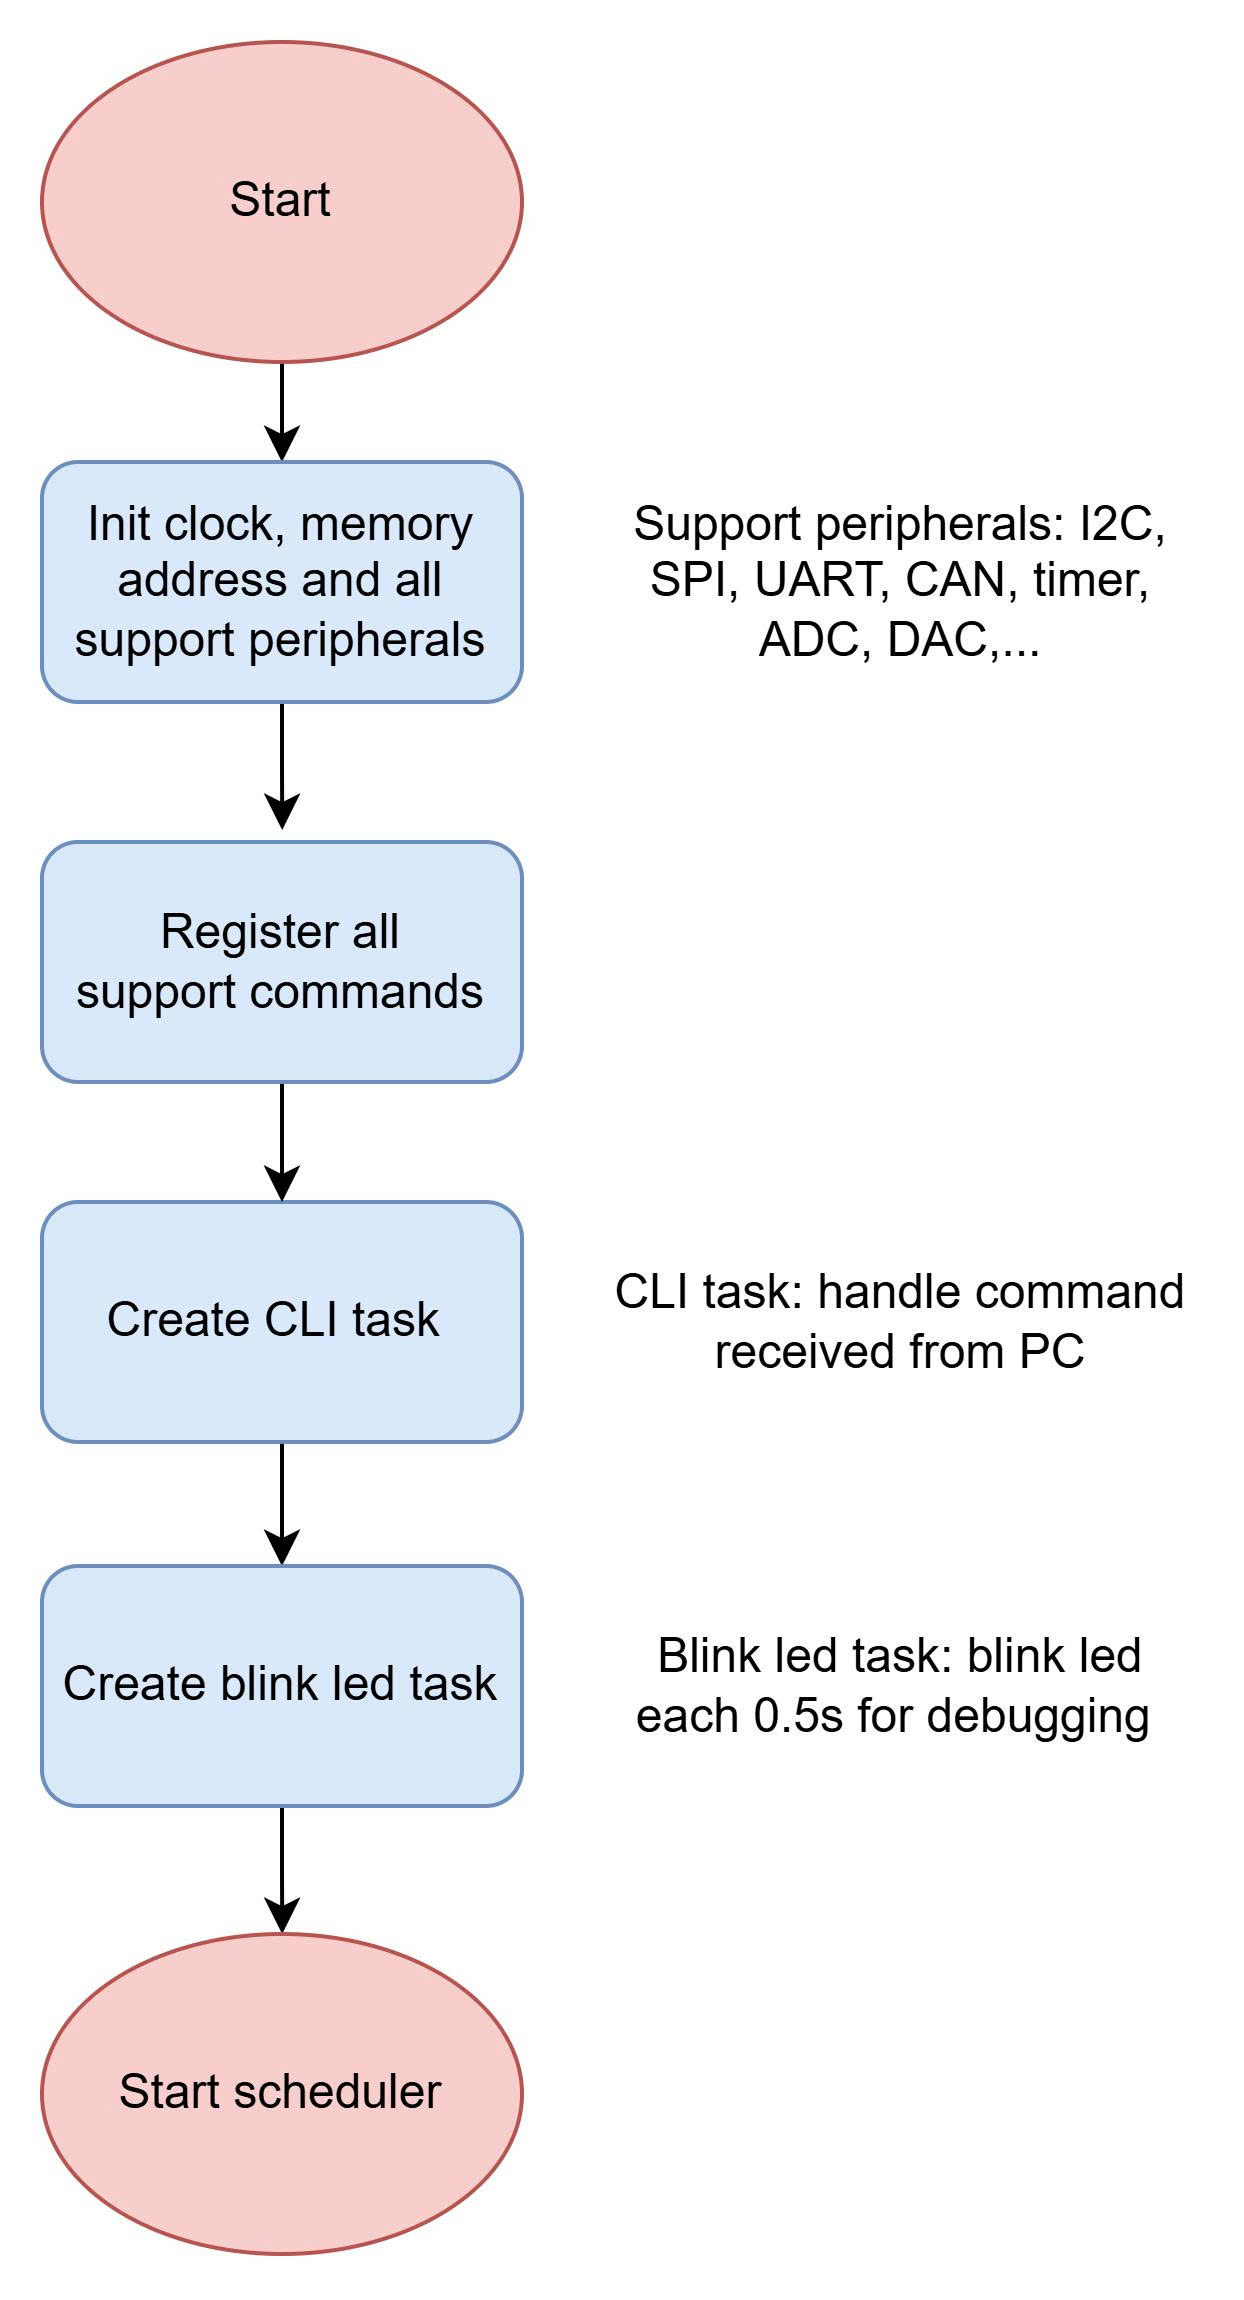
\includegraphics[width=0.3\textwidth]{image/HIL_overview.jpg}
    \caption{Lưu đồ giải thuật tổng quát của hệ thống HIL}
    \label{fig:HIL_overview}
\end{figure}

Quá trình hoạt động của hệ thống HIL bắt đầu bằng giai đoạn khởi tạo. Trong giai đoạn này, vi điều khiển thực hiện cấu hình xung clock hệ thống và khởi tạo các ngoại vi cần thiết như USB, UART, I2C, SPI và các bộ định thời. Việc khởi tạo này đảm bảo các tài nguyên phần cứng sẵn sàng cho quá trình mô phỏng và giao tiếp.

Sau khi hoàn tất khởi tạo, hệ thống tiến hành tạo các task phục vụ cho việc xử lý lệnh từ máy tính và mô phỏng thiết bị ngoại vi. Trong suốt quá trình vận hành, hệ thống HIL liên tục nhận các lệnh cấu hình và điều khiển mô phỏng từ máy tính, sau đó thực hiện các hành vi mô phỏng tương ứng và gửi tín hiệu đến DUT.

Khi DUT phản hồi dữ liệu thông qua các giao thức ngoại vi, hệ thống HIL tiến hành thu thập, xử lý và cập nhật trạng thái mô phỏng. Chu trình này được lặp lại liên tục, đảm bảo hệ thống HIL hoạt động ổn định và đáp ứng kịp thời các yêu cầu kiểm thử firmware.

\section{Lưu đồ giải thuật chi tiết của task xử lý lệnh}

Để đảm bảo khả năng điều khiển linh hoạt từ máy tính, hệ thống HIL triển khai một task chuyên trách cho việc xử lý lệnh. Lưu đồ giải thuật của task này được minh họa trong Hình \ref{fig:HIL_CLI_task}.

\begin{figure}[H]
    \centering
    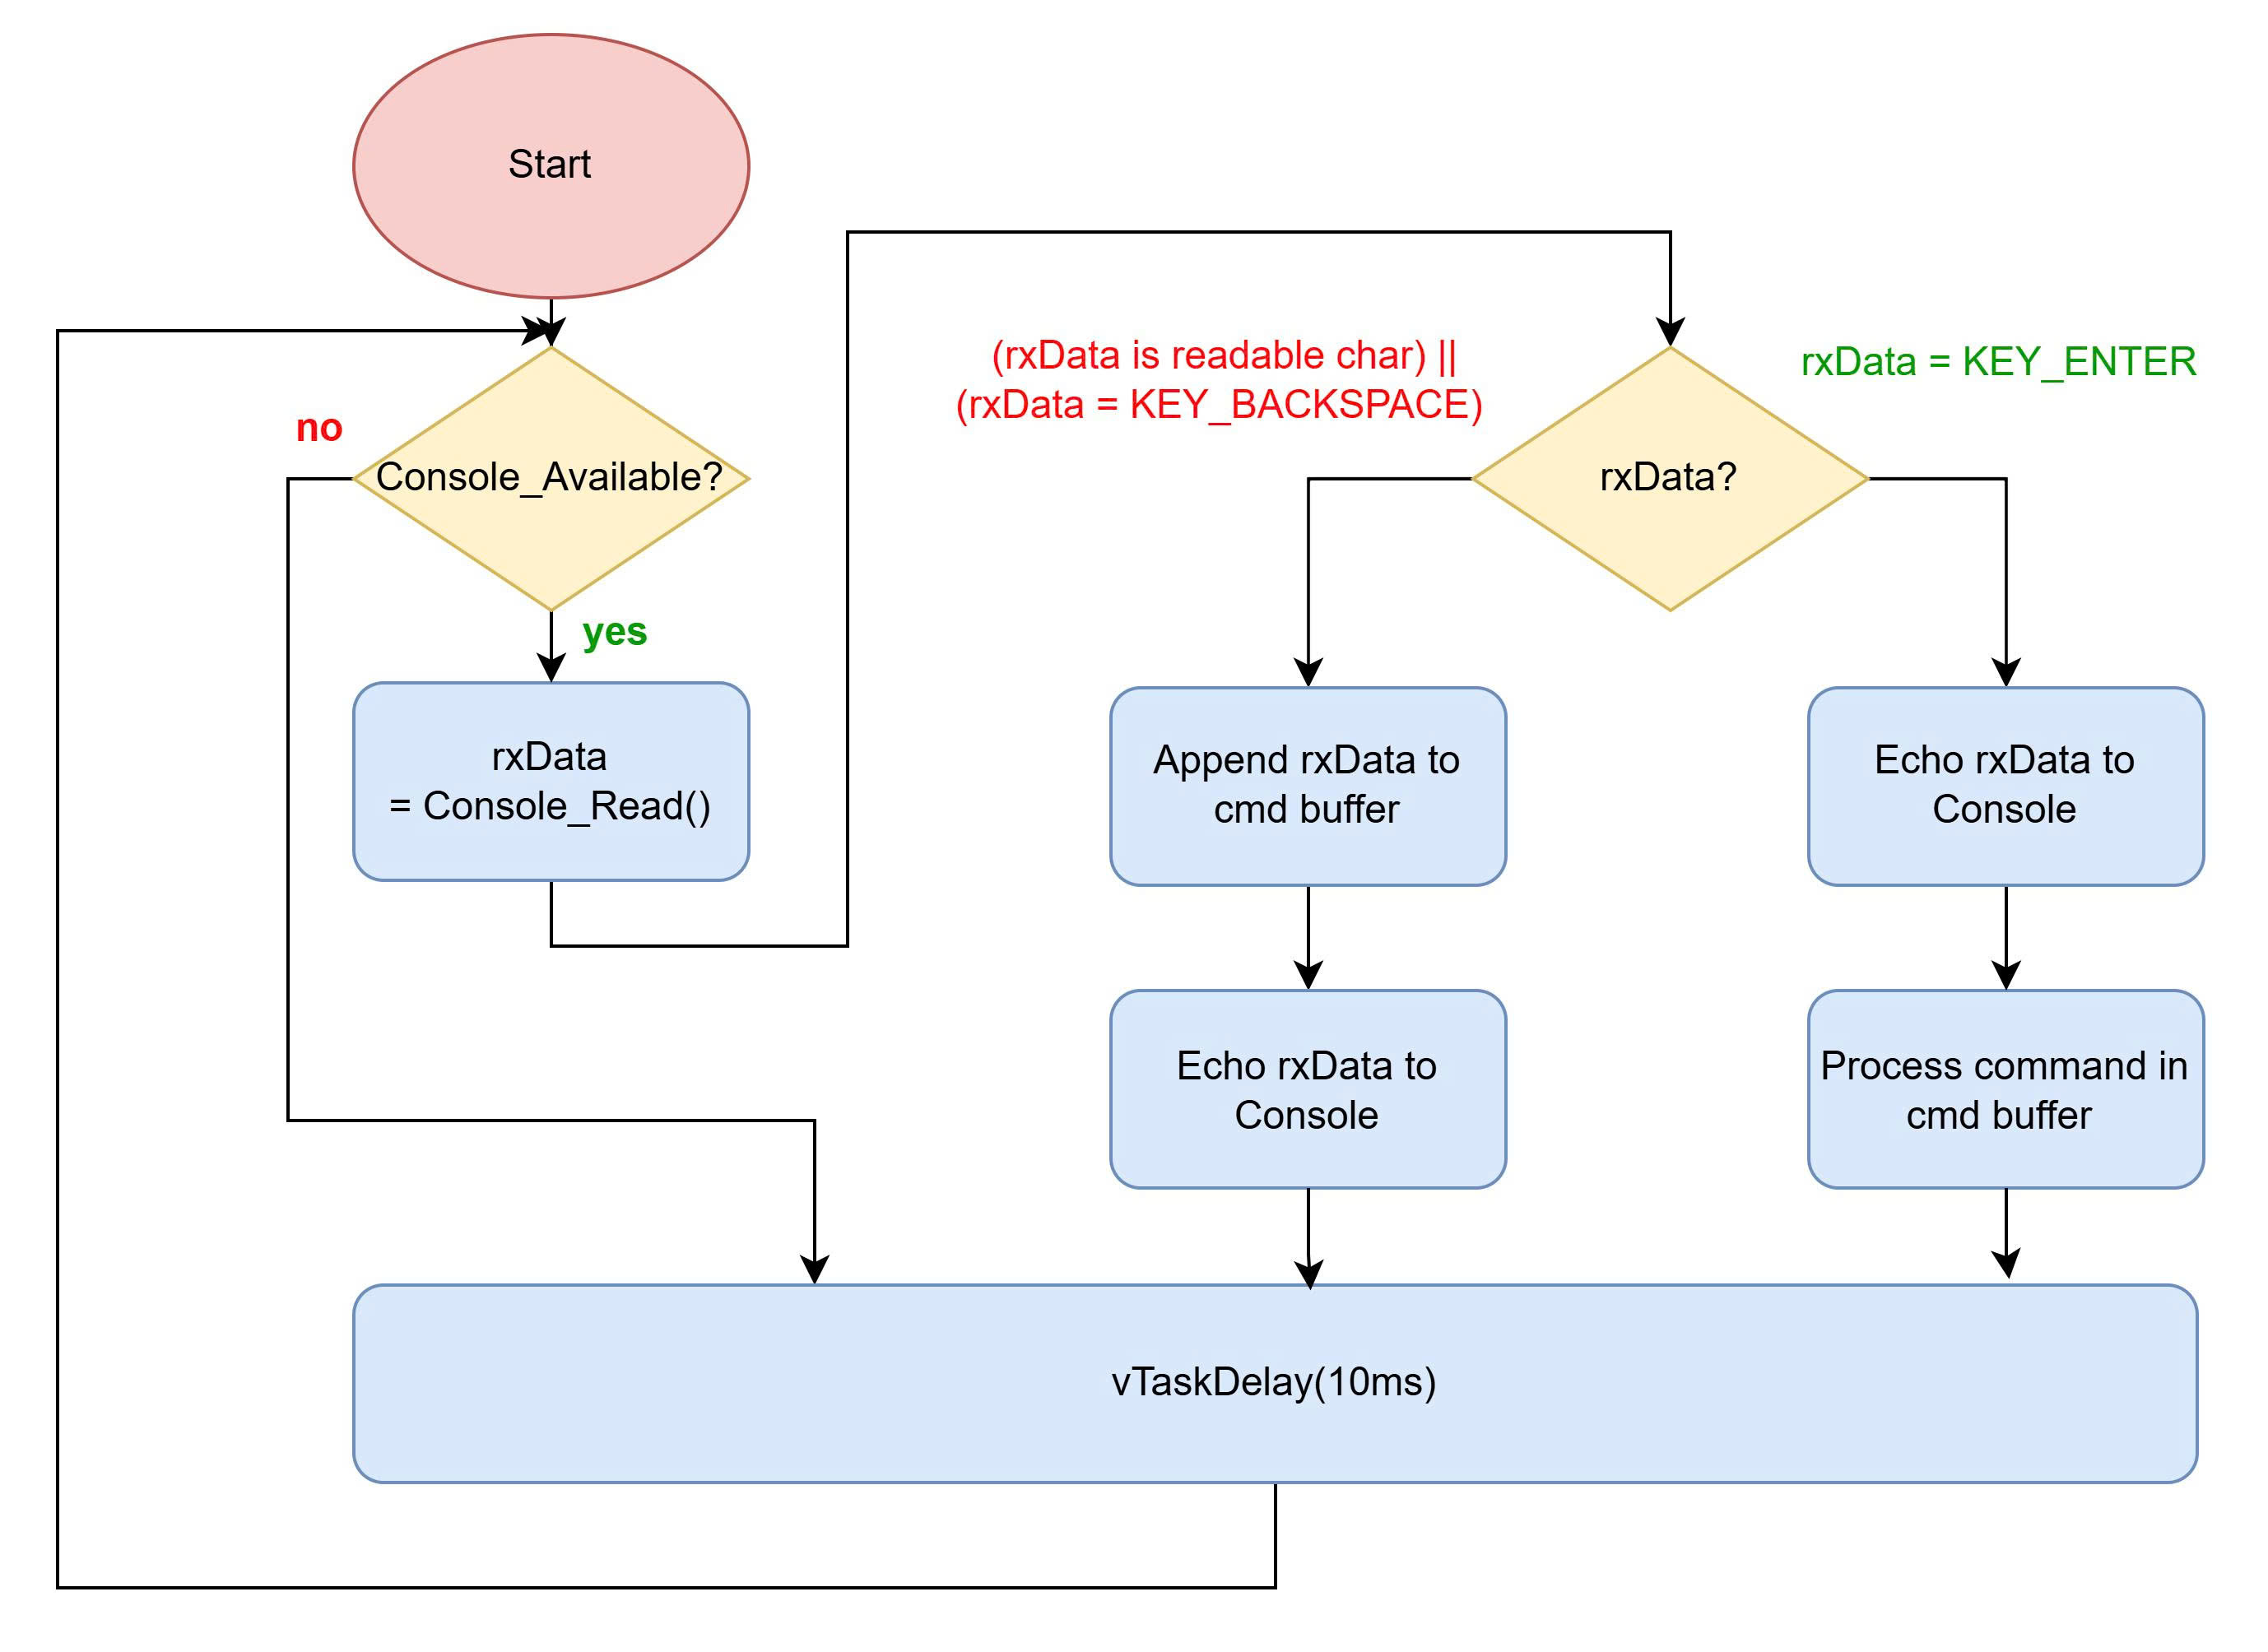
\includegraphics[width=0.7\textwidth]{image/HIL_CLI_task.jpg}
    \caption{Lưu đồ giải thuật của task xử lý lệnh từ máy tính}
    \label{fig:HIL_CLI_task}
\end{figure}

Task xử lý lệnh hoạt động theo cơ chế vòng lặp vô hạn, liên tục chờ dữ liệu từ máy tính thông qua giao tiếp USB. Khi nhận được một lệnh, hệ thống tiến hành phân tích cú pháp và xác định loại lệnh tương ứng.

Đối với các lệnh cấu hình, hệ thống HIL cập nhật các tham số liên quan đến giao tiếp và mô phỏng, bao gồm tốc độ truyền, địa chỉ thiết bị, chế độ hoạt động và định dạng dữ liệu. Các thay đổi này được áp dụng ngay lập tức mà không cần khởi động lại hệ thống.

Trong trường hợp nhận được lệnh điều khiển mô phỏng, hệ thống sẽ kích hoạt mô hình thiết bị ngoại vi tương ứng và thực hiện các thao tác mô phỏng cần thiết để trao đổi dữ liệu với DUT. Nếu lệnh không hợp lệ hoặc không được hỗ trợ, hệ thống gửi thông báo lỗi về máy tính để người dùng xử lý.

Cơ chế này giúp hệ thống HIL luôn sẵn sàng đáp ứng các yêu cầu kiểm thử và nếu cần có thể mở rộng thêm các loại lệnh trong tương lai.

\section{Lưu đồ giải thuật chi tiết mô phỏng thiết bị ngoại vi}
\subsection{Mô phỏng thiết bị ngoại vi giao tiếp I2C}

Hệ thống HIL hỗ trợ mô phỏng các thiết bị ngoại vi giao tiếp I2C nhằm phục vụ kiểm thử firmware của DUT. Trong phạm vi đề tài, hai thiết bị I2C được lựa chọn để mô phỏng là EEPROM và RTC, do đây là các thiết bị phổ biến trong nhiều hệ thống nhúng.

Quy trình mô phỏng thiết bị I2C trong hệ thống HIL được trình bày trong Hình \ref{fig:I2C_device}.

\begin{figure}[H]
    \centering
    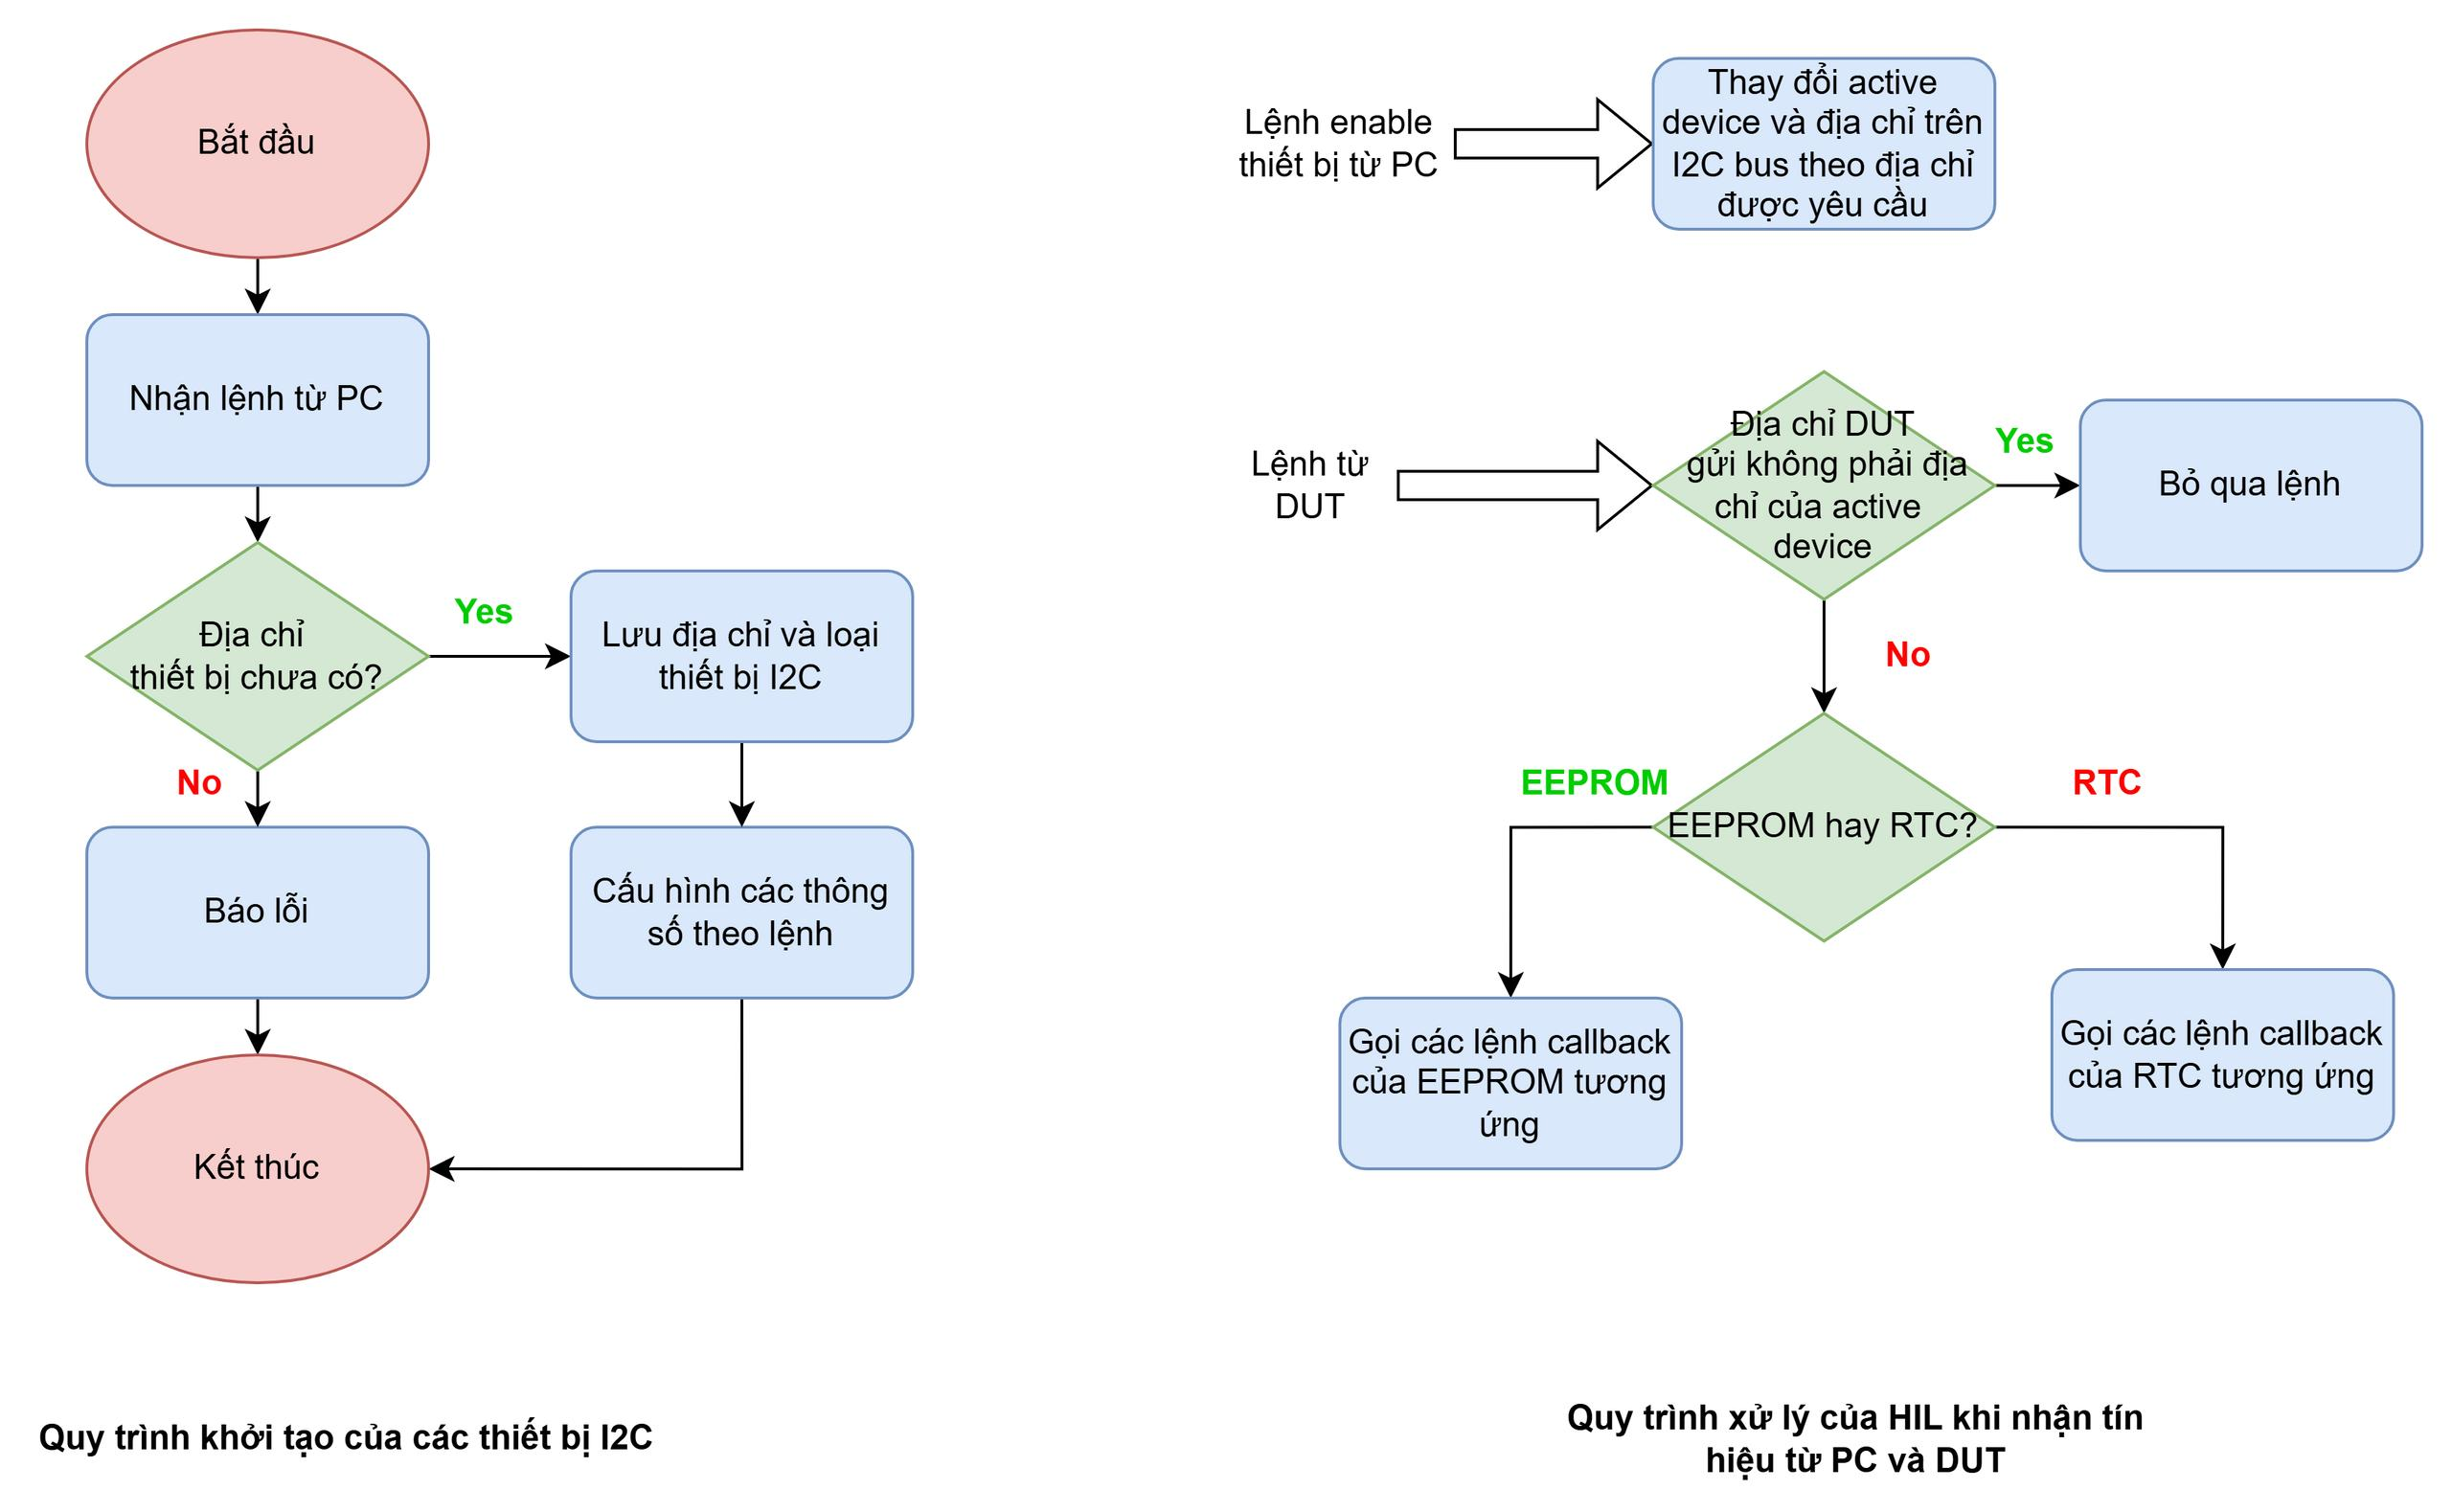
\includegraphics[width=1\textwidth]{image/I2C_device.png}
    \caption{Quy trình mô phỏng thiết bị I2C trong hệ thống HIL}
    \label{fig:I2C_device}
\end{figure}

Để khởi tạo một thiết bị I2C mô phỏng, hệ thống HIL cần nhận lệnh cấu hình từ máy tính, bao gồm loại thiết bị và địa chỉ I2C tương ứng. Do số lượng địa chỉ I2C phần cứng trên vi điều khiển bị giới hạn, các thiết bị I2C trong hệ thống HIL được quản lý hoàn toàn ở mức phần mềm.

Khi nhận được yêu cầu khởi tạo, hệ thống kiểm tra xem địa chỉ I2C đã được sử dụng hay chưa. Nếu địa chỉ đã tồn tại trong danh sách quản lý, hệ thống từ chối khởi tạo và gửi thông báo lỗi về máy tính. Ngược lại, nếu địa chỉ hợp lệ, thiết bị mô phỏng được khởi tạo và lưu vào danh sách quản lý thiết bị I2C.

Trong quá trình DUT giao tiếp trên bus I2C, hệ thống HIL giám sát địa chỉ truy cập và kích hoạt mô hình thiết bị tương ứng. Dữ liệu phản hồi được tạo ra dựa trên mô hình hành vi của thiết bị, đảm bảo tính tương đương với thiết bị thực.

Đối với thiết bị EEPROM, hệ thống HIL mô phỏng bộ nhớ lưu trữ theo từng trang, trong đó dữ liệu ghi từ DUT được đệm tạm và chỉ được ghi chính thức vào vùng nhớ mô phỏng khi phiên giao tiếp I2C kết thúc. Cách tiếp cận này đảm bảo hành vi ghi dữ liệu tương đương với EEPROM thực, bao gồm cơ chế tự tăng địa chỉ và giới hạn kích thước trang.

Đối với thiết bị RTC, hệ thống HIL mô phỏng tập thanh ghi thời gian theo chuẩn của DS1307 và sử dụng bộ định thời nội để cập nhật giá trị thời gian thực theo chu kỳ 1 giây. DUT có thể thực hiện các thao tác đọc và ghi để lấy hoặc thiết lập thời gian, trong đó dữ liệu được mã hóa theo định dạng BCD giống với thiết bị phần cứng thực tế.

\subsection{Mô phỏng thiết bị ngoại vi giao tiếp SPI}

Bên cạnh giao tiếp I2C, hệ thống HIL còn hỗ trợ mô phỏng các thiết bị ngoại vi sử dụng giao thức SPI nhằm kiểm thử các chức năng firmware của DUT liên quan đến bộ nhớ ngoài. Trong phạm vi đề tài, thiết bị SPI được lựa chọn để mô phỏng là bộ nhớ Flash W25Q, một linh kiện phổ biến trong các hệ thống nhúng dùng để lưu trữ chương trình và dữ liệu.

Thiết bị Flash SPI được mô phỏng theo mô hình slave, trong đó hệ thống HIL đóng vai trò phản hồi các lệnh truy cập từ DUT thông qua bus SPI. Toàn bộ nội dung bộ nhớ Flash được mô phỏng bằng vùng nhớ RAM trong vi điều khiển của HIL, cho phép truy cập nhanh và linh hoạt trong quá trình kiểm thử.

Quy trình mô phỏng thiết bị SPI trong hệ thống HIL được trình bày trong Hình~\ref{fig:SPI_flash}.

\begin{figure}[H]
    \centering
    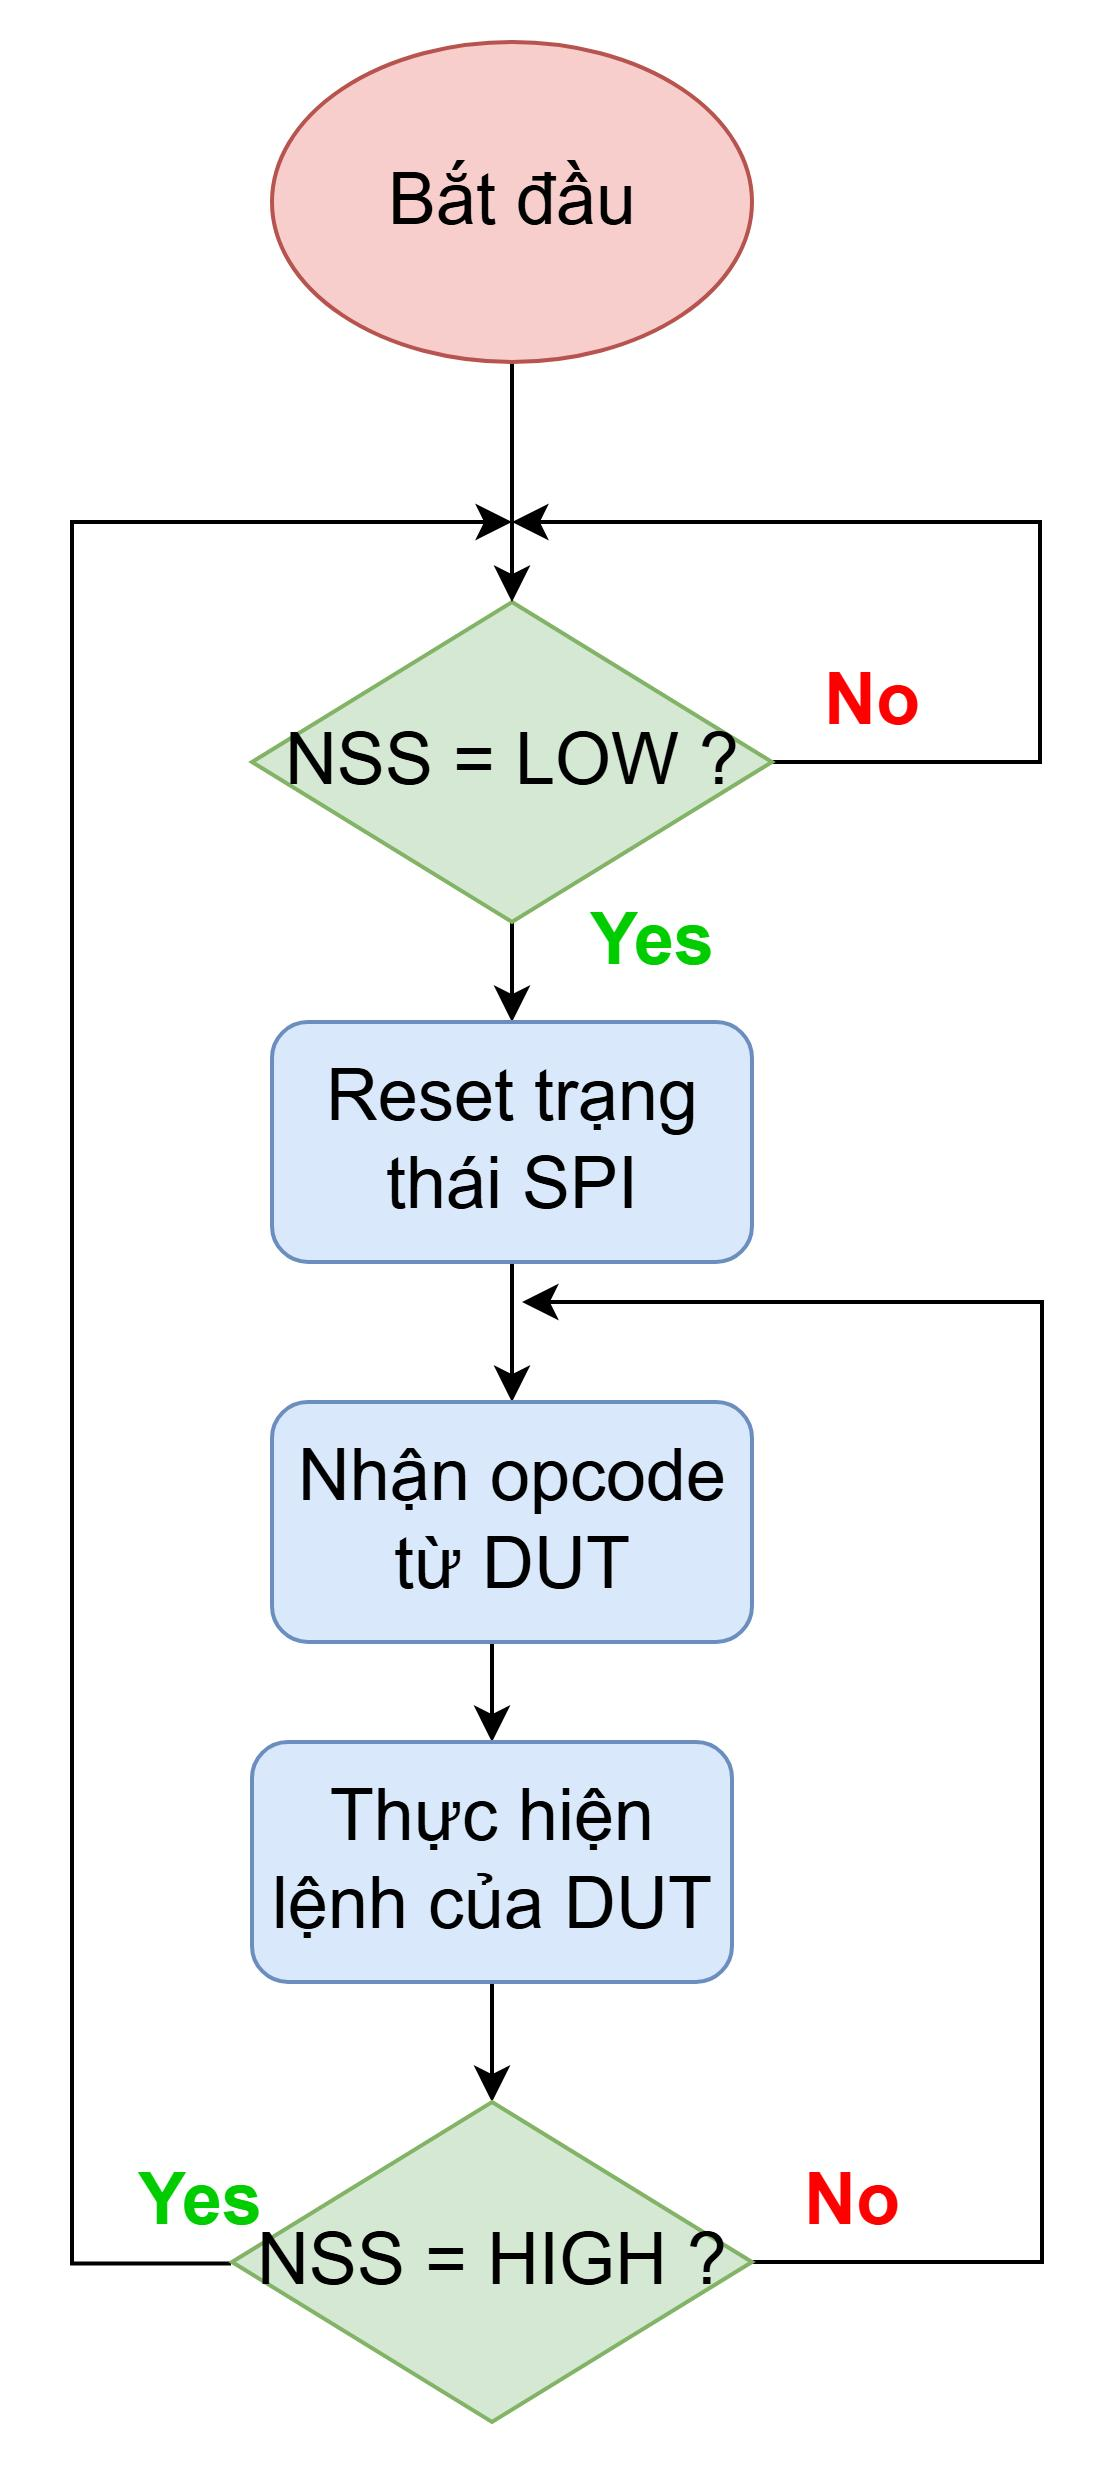
\includegraphics[width=0.35\textwidth]{image/SPI_flash.png}
    \caption{Quy trình mô phỏng bộ nhớ SPI flash trong hệ thống HIL}
    \label{fig:SPI_flash}
\end{figure}

Quá trình mô phỏng SPI bắt đầu khi DUT kích hoạt tín hiệu Chip Select (NSS) ở mức thấp, báo hiệu một phiên giao tiếp SPI mới. Hệ thống HIL sử dụng ngắt ngoài để phát hiện sự kiện này và tiến hành khởi tạo lại các biến trạng thái nội bộ, đảm bảo mỗi transaction SPI được xử lý độc lập và chính xác.

Byte dữ liệu đầu tiên được DUT truyền đến được xem là lệnh điều khiển (opcode). Dựa trên opcode nhận được, hệ thống HIL xác định loại lệnh tương ứng và chuyển sang trạng thái xử lý phù hợp. Trong phạm vi đề tài, các lệnh cơ bản của Flash SPI như đọc ID, đọc dữ liệu, ghi dữ liệu và xóa bộ nhớ được mô phỏng.

Đối với lệnh đọc ID, hệ thống HIL phản hồi lần lượt các byte định danh thiết bị, cho phép DUT xác nhận đúng loại Flash đang được sử dụng. Với lệnh đọc dữ liệu, sau khi nhận đủ địa chỉ truy cập, hệ thống bắt đầu truyền dữ liệu từ bộ nhớ mô phỏng về DUT, đồng thời tự động tăng địa chỉ để mô phỏng cơ chế đọc liên tục của Flash thực.

Trong trường hợp lệnh ghi dữ liệu, hệ thống HIL tiếp nhận dữ liệu từ DUT và lưu vào vùng nhớ mô phỏng tương ứng với địa chỉ đã chỉ định. Đối với lệnh xóa bộ nhớ, toàn bộ vùng nhớ mô phỏng được đưa về trạng thái mặc định, tương đương với quá trình xóa chip của Flash thực tế.

Trong suốt quá trình giao tiếp SPI, hệ thống HIL gửi các byte dummy khi cần thiết nhằm duy trì xung clock và đảm bảo đồng bộ truyền nhận giữa master và slave. Cơ chế này giúp DUT hoạt động bình thường mà không cần thay đổi firmware khi chuyển từ thiết bị Flash thực sang Flash mô phỏng.

Việc mô phỏng thiết bị SPI trong hệ thống HIL cho phép kiểm thử đầy đủ các chức năng liên quan đến bộ nhớ ngoài của DUT mà không cần sử dụng phần cứng Flash thật. Điều này giúp giảm chi phí phần cứng, đồng thời tăng tính linh hoạt và khả năng tự động hóa trong quá trình phát triển và kiểm thử firmware nhúng.

\section{Lưu đồ giải thuật xử lý các ngoại vi}
\subsection{Xử lý UART/CAN}
\begin{figure}[H]
    \centering
    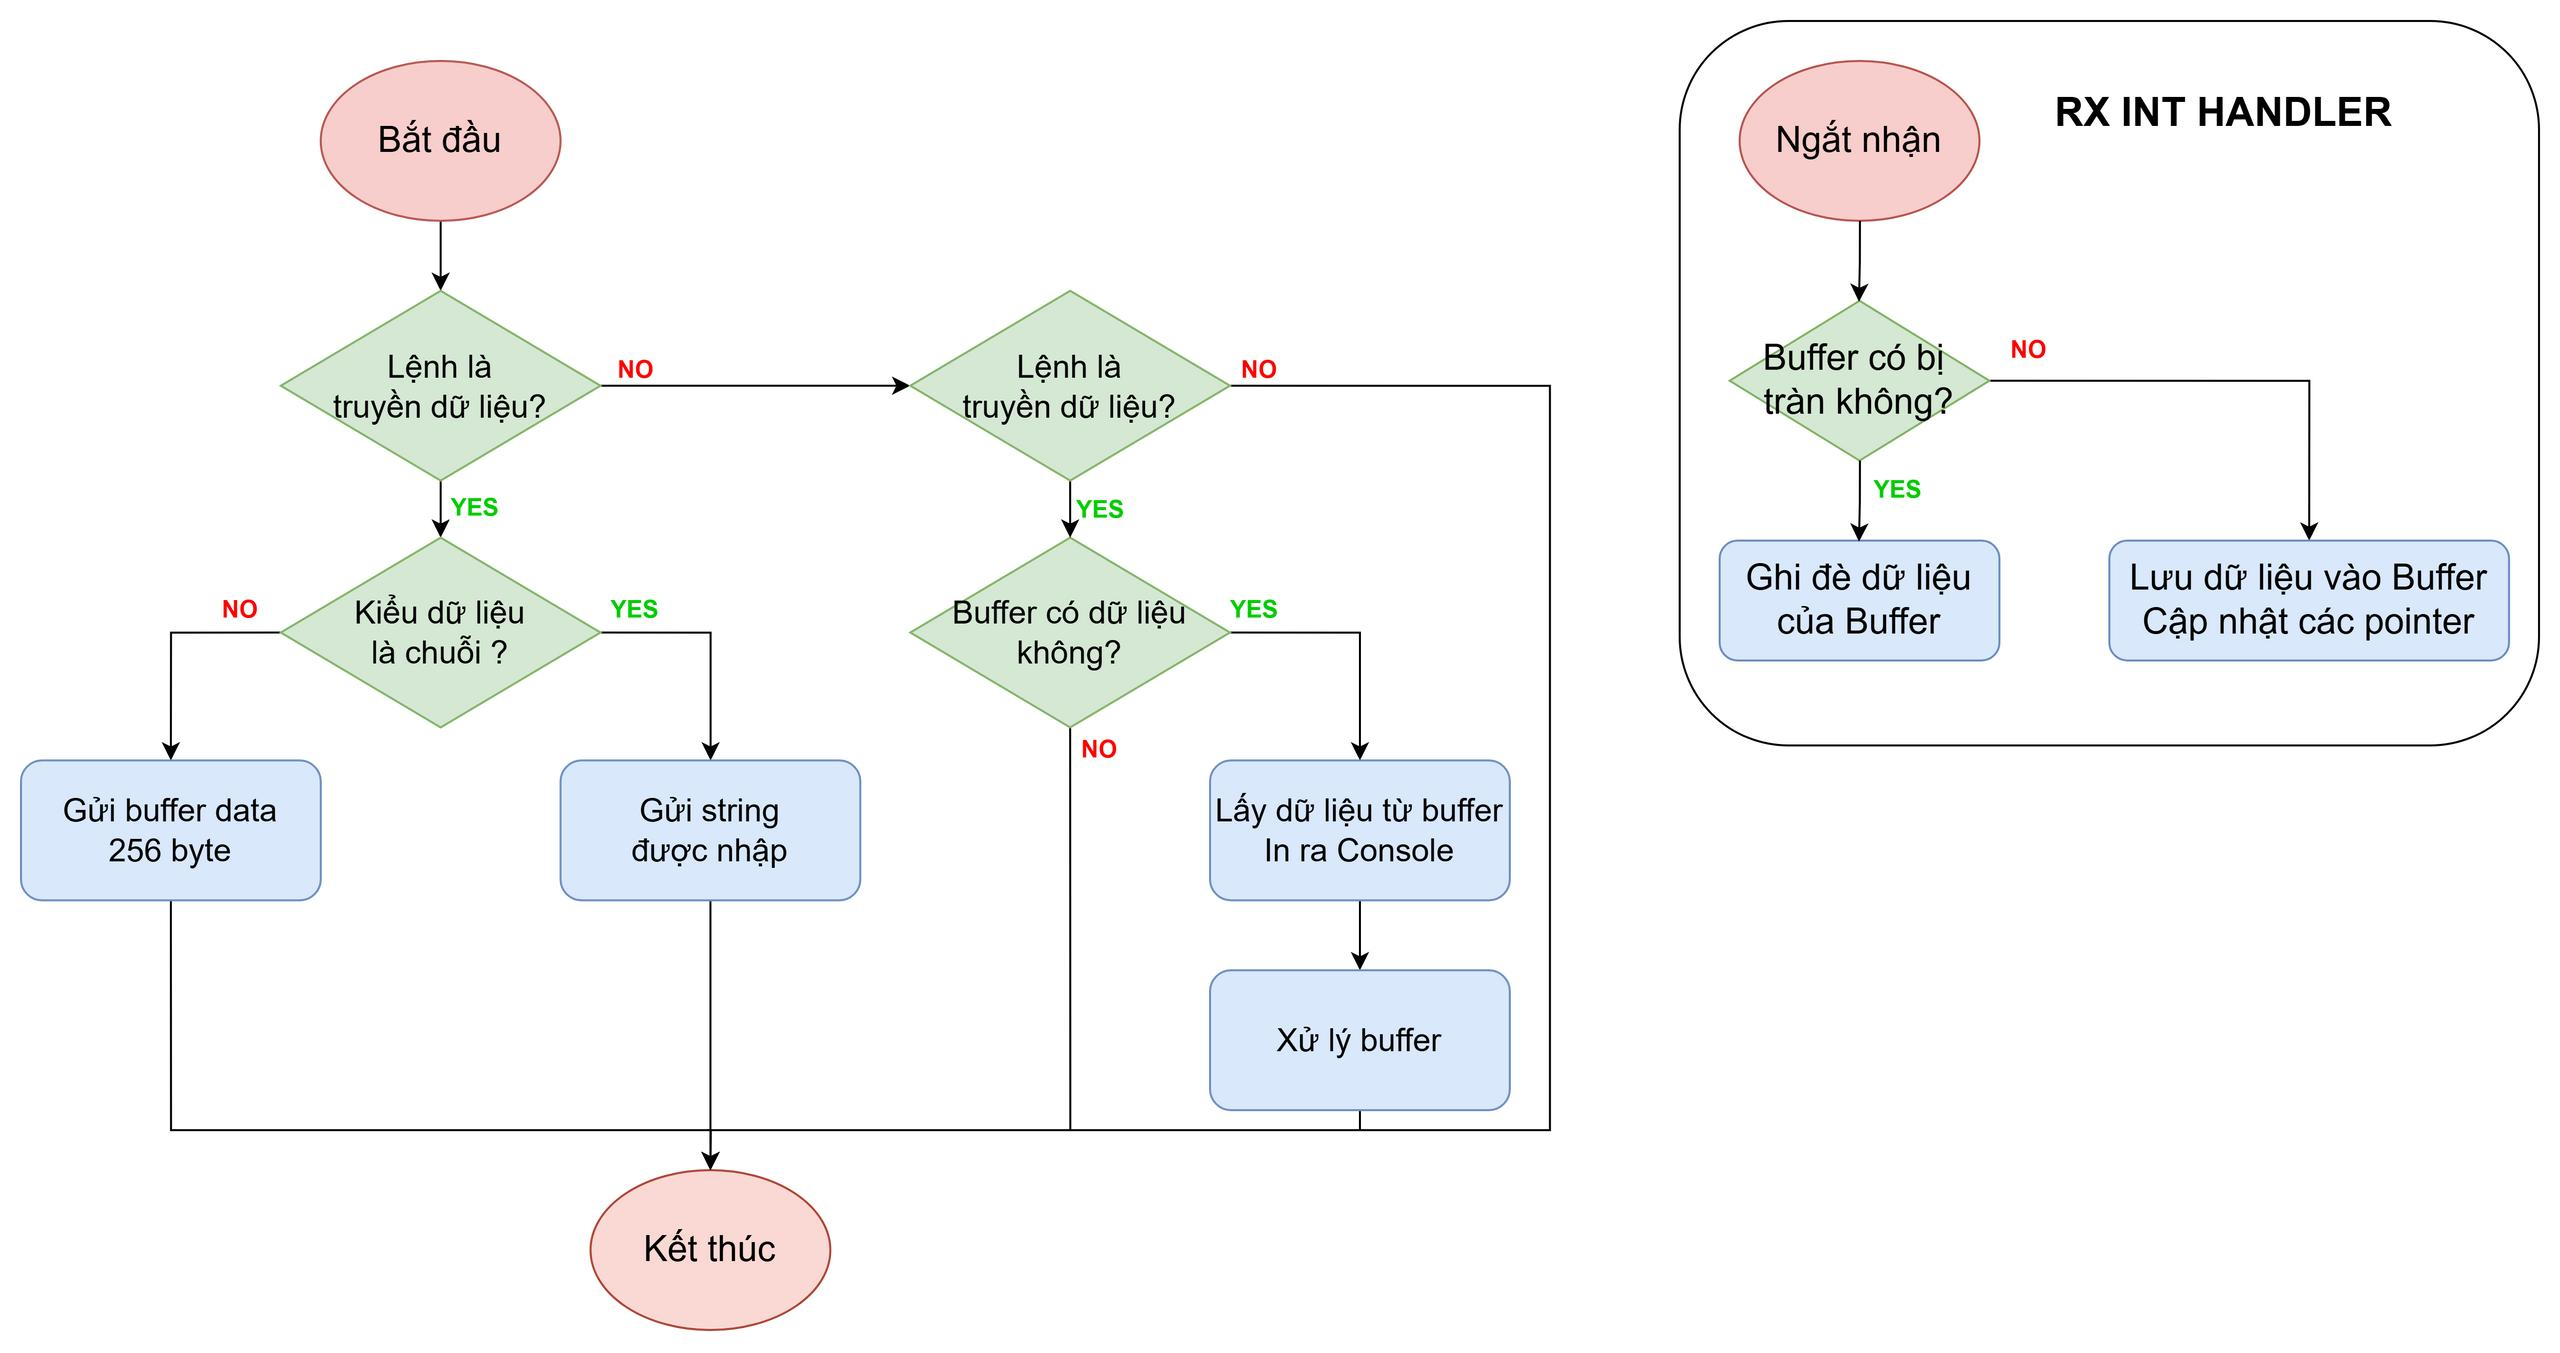
\includegraphics[width=1\textwidth]{image/hil_uart_can.jpg}
    \caption{Lưu đồ giải thuật giao tiếp UART và CAN}
    \label{fig:hil_uart_can}
\end{figure}
Lưu đồ giải thuật trên mô tả quá trình xử lý truyền và nhận dữ liệu của khối giao tiếp UART và CAN trong hệ thống.
Khi hệ thống hoạt động, chương trình sẽ kiểm tra lệnh cần xử lý. Nếu là lệnh truyền dữ liệu, hệ thống sẽ xác định kiểu dữ liệu cần gửi.
Đối với dữ liệu dạng buffer, HIL sẽ gửi toàn bộ khối dữ liệu có kích thước 256 byte thông qua giao thức UART hoặc CAN với các giá trị tăng dần từ 0x00 $\rightarrow$ 0xFF và lặp lại.
Trong trường hợp dữ liệu cần truyền là chuỗi ký tự, hệ thống sẽ gửi chuỗi được nhập đó đến DUT. Sau khi hoàn tất quá trình truyền, hệ thống chuyển sang trạng thái kết thúc truyền và sẵn sàng cho các yêu cầu tiếp theo.

Đối với lệnh truyền dữ liệu, chương trình sẽ kiểm tra trạng thái của buffer nhận để xác định có dữ liệu mới hay không. Nếu buffer chưa có dữ liệu, quá trình đọc sẽ kết thúc.
Nếu buffer đã chứa dữ liệu, chương trình sẽ lấy dữ liệu từ buffer và hiển thị ra console nhằm phục vụ cho mục đích giám sát.
Dữ liệu sẽ được ghi vào buffer trong quá trinh ngắt. Nếu buffer chưa đầy, dữ liệu mới sẽ được lưu vào buffer đồng thời cập nhật các pointer quản lý vị trí đọc và ghi.
Trong trường hợp buffer bị tràn, hệ thống sẽ ghi đè dữ liệu cũ của buffer.

Cơ chế ngắt nhận dữ liệu sẽ được phần cứng tự động kích hoạt mỗi khi có một khung truyền được gửi đến. Tuy nhiên dựa vào Hình \ref{fig:uart_frame} và Hình \ref{fig:can_frame} có thể thấy UART và CAN có khung truyền khác nhau.
Với UART, mỗi khung truyền chỉ có 1 byte dữ liệu nhưng giao thức CAN có thể linh hoạt độ dài của dữ liệu bằng trường DLC cho phép độ dài vùng dữ liệu dao động từ 0 - 8 byte.
Chính vì thế quá trình xử lý ngắt cho UART và CAN được thiết kế với vài điểm khác biệt.
\begin{figure}[H]
    \centering
    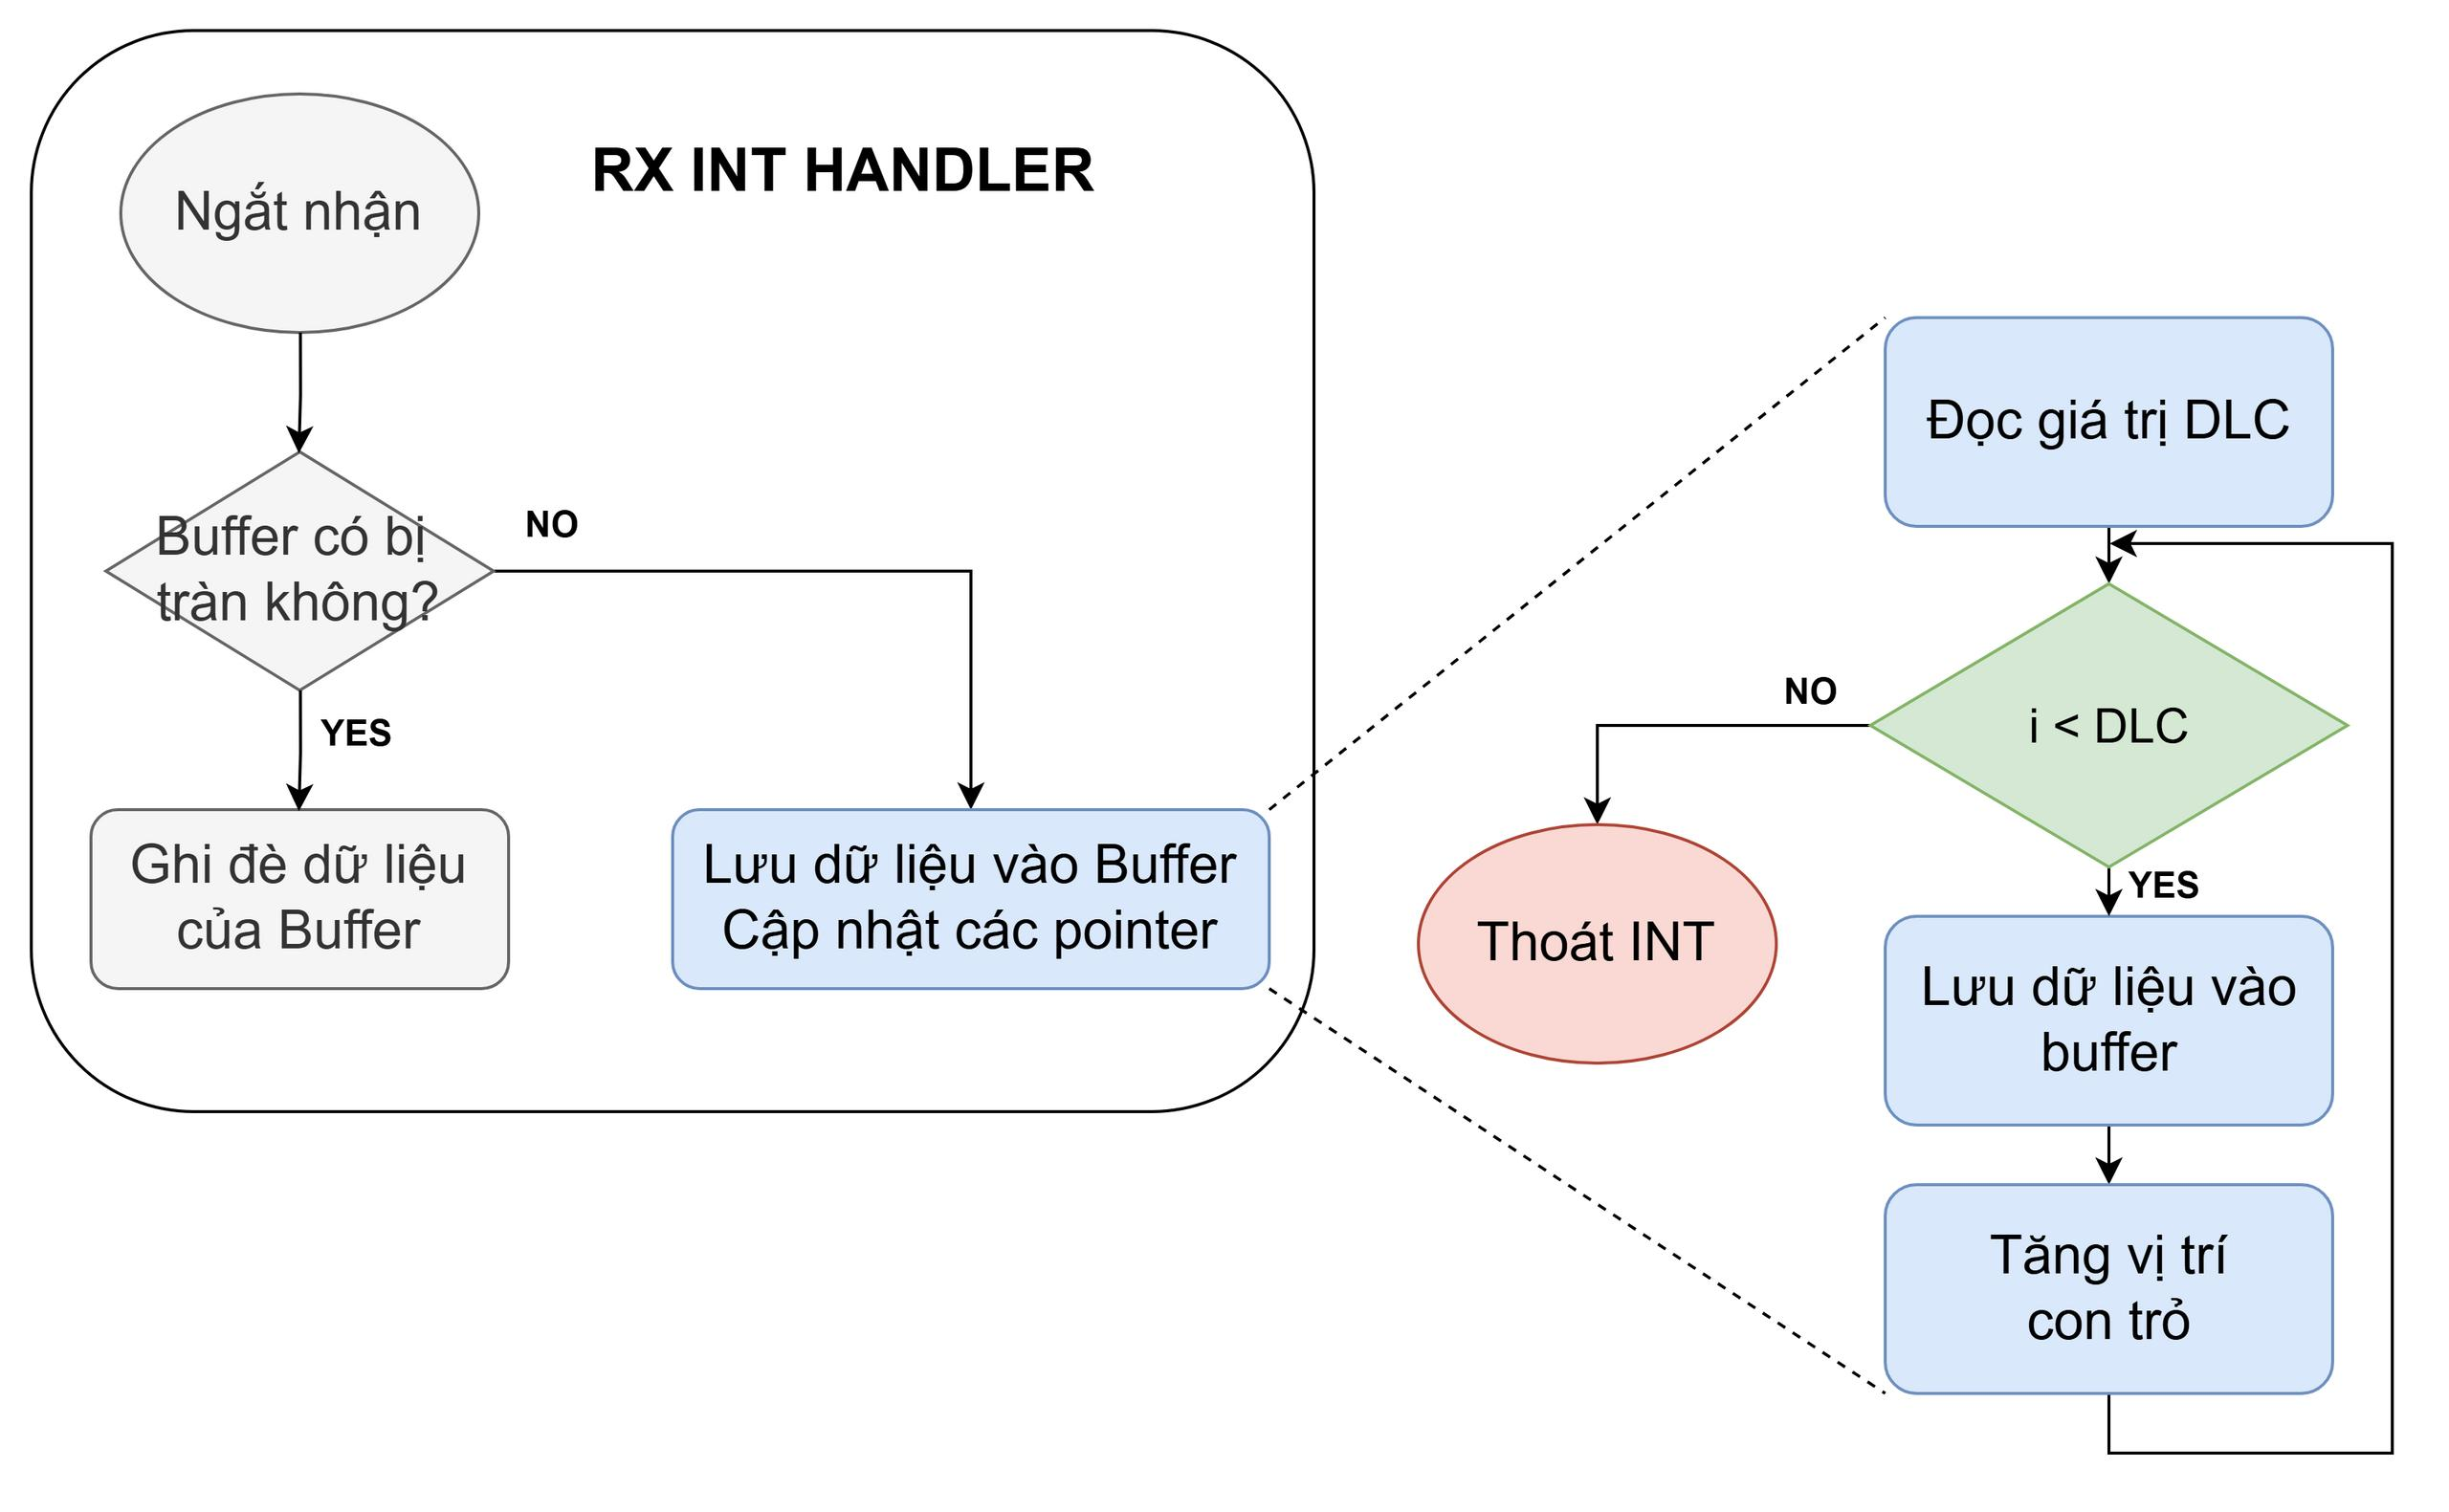
\includegraphics[width=0.65\textwidth]{image/hil_can.jpg}
    \caption{Lưu đồ giải thuật xử lý ngắt nhận của giao thức CAN}
    \label{fig:hil_can}
\end{figure}
Hình \ref{fig:hil_can} mô tả thuật toán xử lý dữ liệu cho giao thức CAN khi có ngắt nhận. Khi một frame CAN được nhận, HIL sẽ trước tiên đọc giá trị từ trường DLC (Data Length Code) để xác định số byte dữ liệu cần xử lý. 
Dựa trên giá trị này, hệ thống thực hiện vòng lặp để lần lượt đọc từng byte dữ liệu và lưu vào buffer. Sau mỗi lần lưu, con trỏ buffer sẽ được tăng lên để chuẩn bị cho vị trí lưu trữ tiếp theo.
Quá trình này tiếp tục cho đến khi toàn bộ số byte tương ứng với giá trị DLC được xử lý hoàn tất, sau đó chương trình sẽ thoát khỏi trình phục vụ ngắt.

Đối với giao tiếp UART, cơ chế xử lý đơn giản hơn do dữ liệu được nhận theo từng byte riêng lẻ. Mỗi khi xảy ra ngắt nhận, hệ thống sẽ đọc một byte dữ liệu và lưu trực tiếp vào buffer. Sau đó, con trỏ buffer được tăng lên để chuẩn bị cho lần nhận tiếp theo.

\subsection{Xử lý ADC/DAC}
\begin{figure}[H]
    \centering
    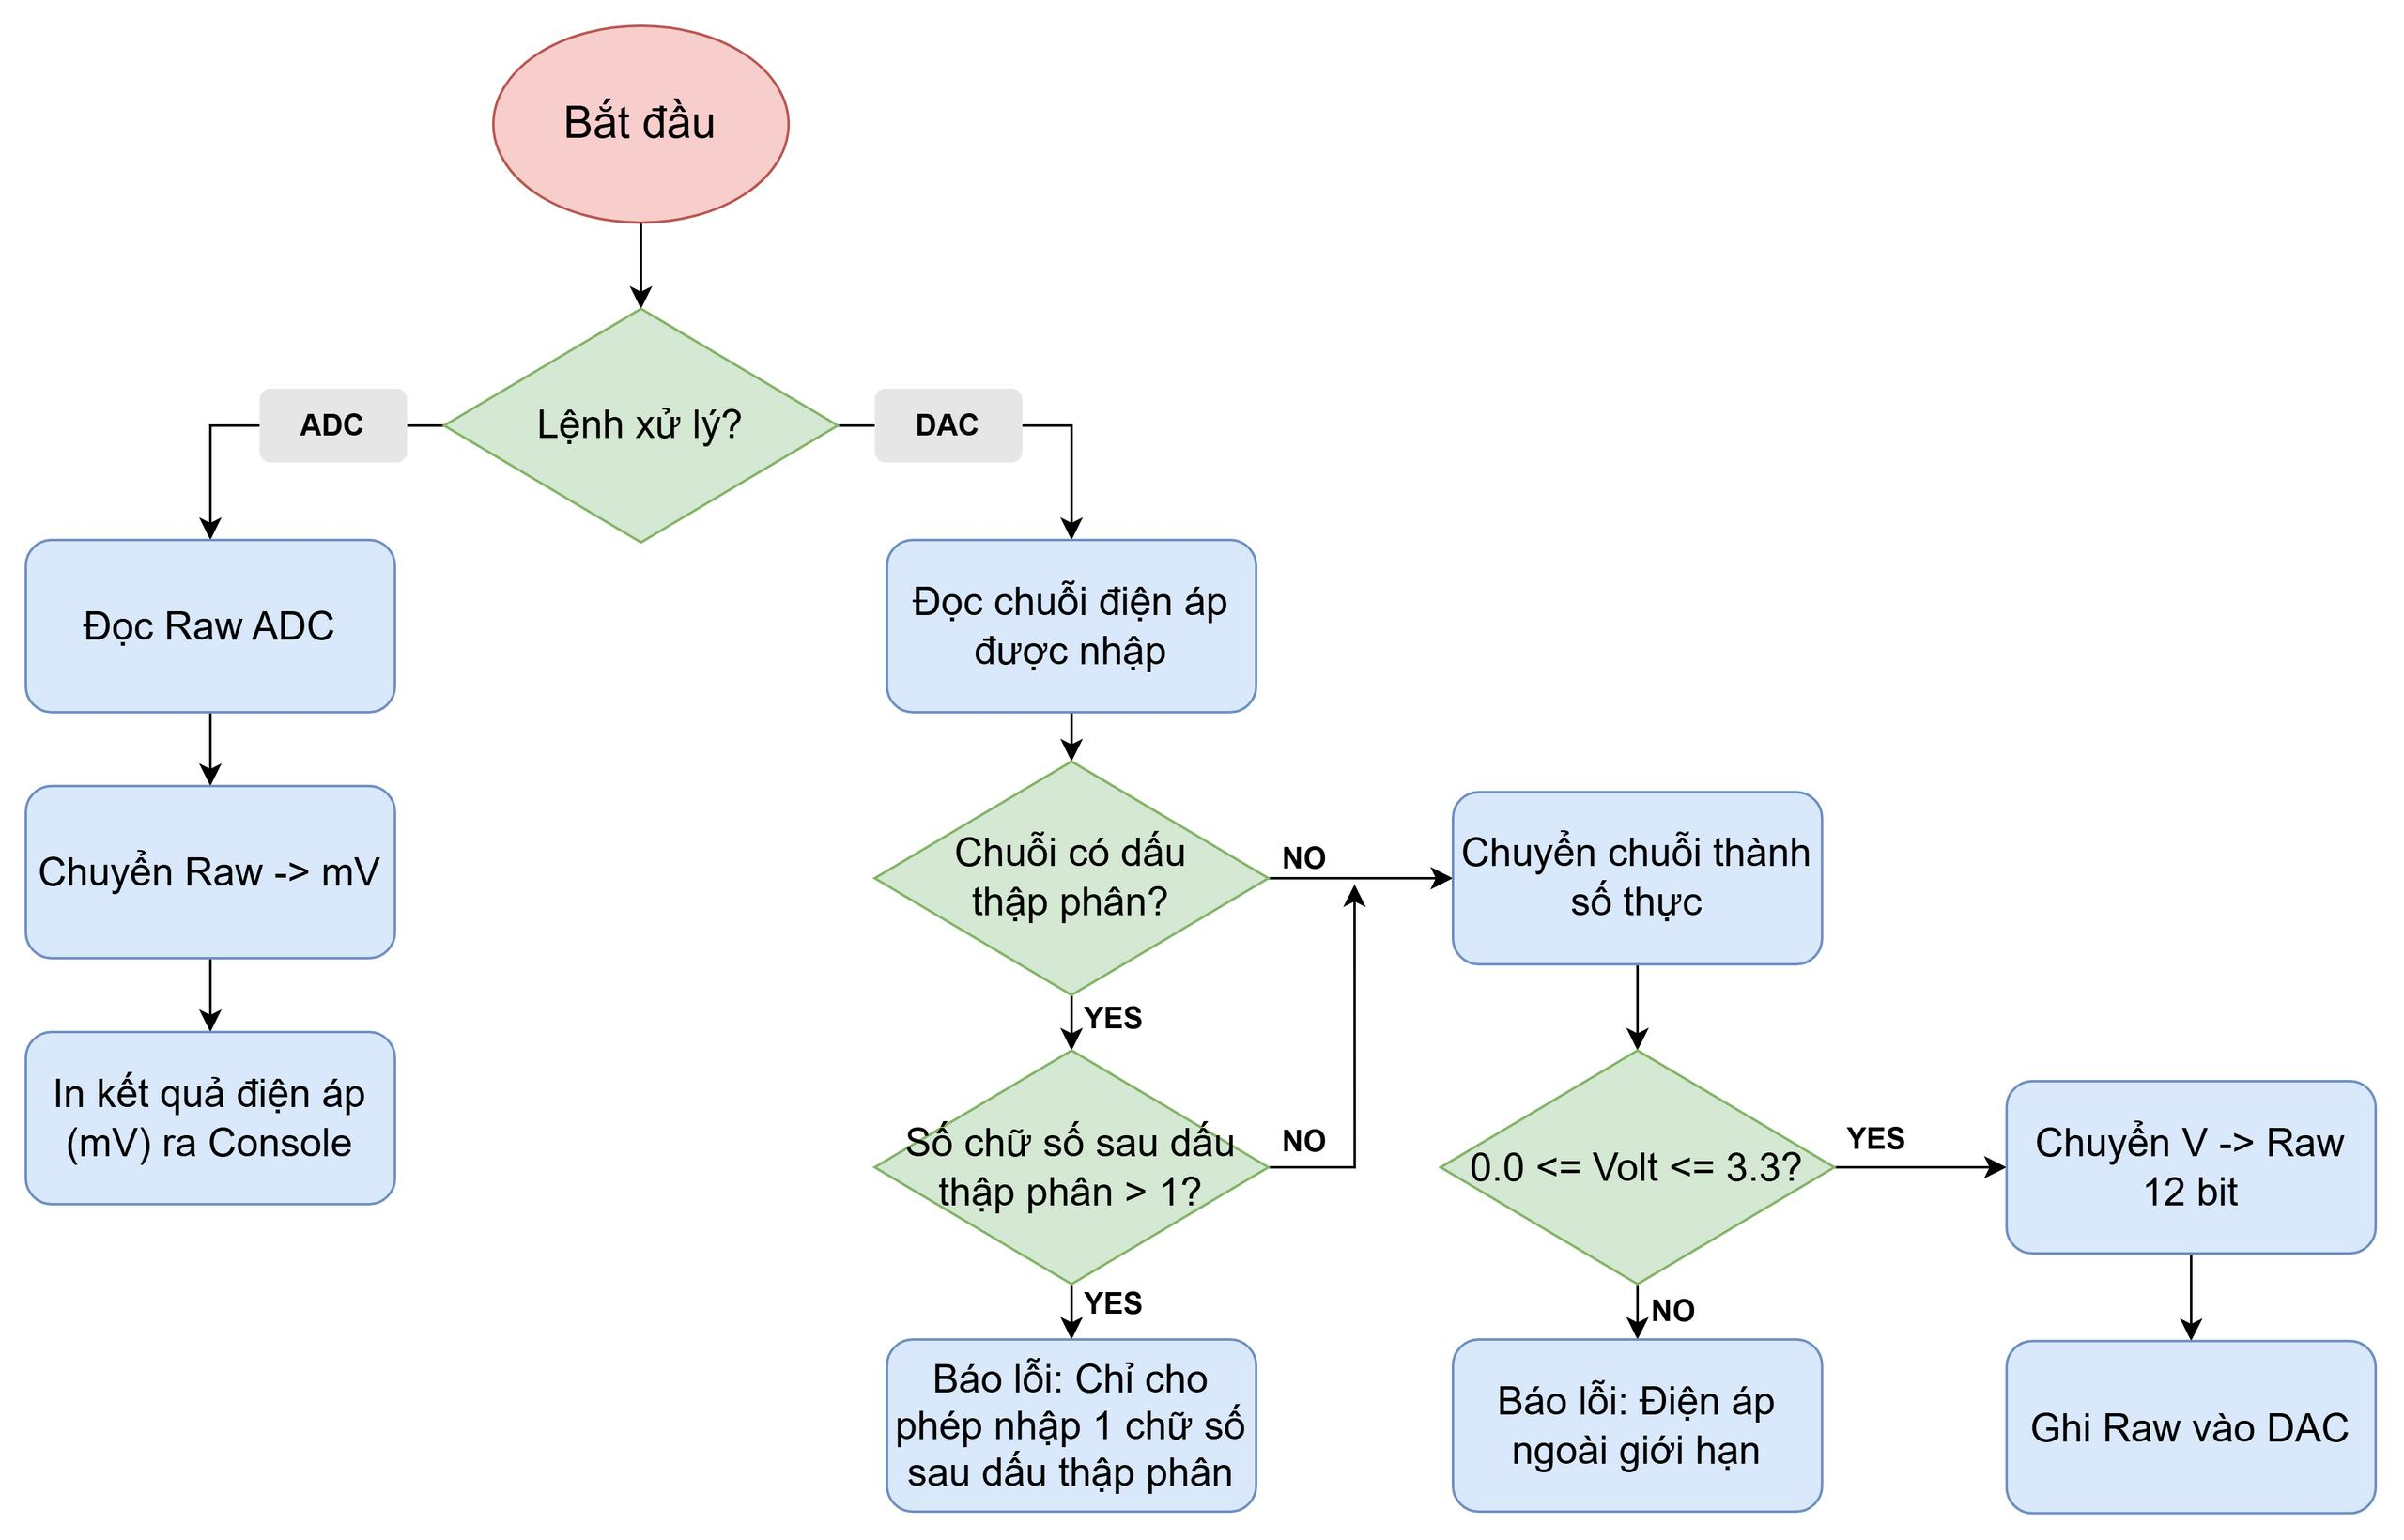
\includegraphics[width=1\textwidth]{image/hil_adc_dac.jpg}
    \caption{Lưu đồ giải thuật xử lý ADC và DAC}
    \label{fig:hil_adc_dac}
\end{figure}
Lưu đồ mô tả giải thuật xử lý cho ADC và DAC. Khi nhận được lệnh đọc ADC, HIL sẽ thu thập giá trị Raw 12 bit từ ADC. Giá trị này được chuyển đổi sang mức điện áp $mV$ theo công thức: $V_{mV}=\dfrac{Raw \cdot 3.3}{2^{12}-1} \cdot 1000$ và tiến hành in kết quả lên Console.

Đối với lệnh cấu hình mức điện áp cho DAC, hệ thống sẽ nhận giá trị điện áp mong muốn dưới dạng một chuỗi ký tự.
Ở bước đầu sẽ kiểm tra trong chuỗi có dấu thập phân hay không. Nếu có thì cần phải đảm bảo sau dấu thập phân chỉ có 1 chữ số.
Sau đó chuỗi sẽ được chuyển thành số thực và tiếp tục kiểm tra giá trị điện áp có nằm trong dải điện áp an toàn của phần cứng từ 0.0V đến 3.3V không.
Khi có các vi phạm trong quá trình kiểm tra trên, hệ thống sẽ không thực thi và in ra thông báo lỗi. Khi mức điện áp đầu vào được xác nhận là hoàn toàn hợp lệ, thuật toán sẽ áp dụng phương trình chuyển đổi ngược $Raw_{DAC} = \dfrac{V_{input}}{3.3} \cdot 4095$ để ánh xạ mức điện áp thành một giá trị nguyên 12 bit tương ứng.
Cuối cùng, giá trị này được ghi vào DAC và xuất tín hiệu điện áp.

\subsection{Tạo sóng sin / sóng tam giác}
Về bản chất, tín hiệu Analog là tín hiệu liên tục theo thời gian và có thể được biểu diễn bởi các mức điện áp thay đổi liên tục.
Để có thể tái tạo tín hiệu Analog bằng hệ thống số, tín hiệu sẽ được cập nhật thành nhiều giá trị điện áp rời rạc tại các thời điểm khác nhau. Nếu khoảng thời gian giữa các lần cập nhật càng nhỏ, hay nói cách khác tần số lấy mẫu càng cao, thì tín hiệu tạo ra sẽ càng tiệm cận với dạng sóng Analog ban đầu và trở nên mượt hơn.
Tần số thực hiện các lần cập nhật này được gọi là tần số lấy mẫu ($f_{sample}$).
\begin{figure}[H]
    \centering
    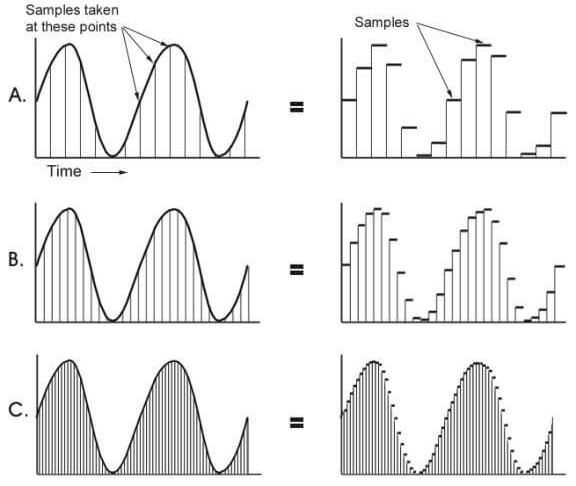
\includegraphics[width=0.6\textwidth]{image/hil_wave_sample.jpg}
    \caption{Quá trình lấy mẫu để tái tạo tín hiệu analog}
    \label{fig:hil_can}
\end{figure}

Từ lý thuyết trên, HIL sẽ thực hiện chức năng tạo sóng sin / tam giác thông qua việc kết hợp DAC, DMA và Timer để tối ưu hóa hiệu suất và đảm bảo tính thời gian thực.
Tần số của Timer ($f_{sample}$) sẽ kích hoạt sự kiện để DMA lấy 1 giá trị trong mảng vùng nhớ để nạp vào DAC và để tạo nên một chu kỳ sóng hoàn chỉnh ta cần $N$ mẫu.
Từ đó ta có thể tính được tần số của sóng như sau:
\begin{equation}
    f_{wave} = \dfrac{f_{sample}}{N}
    \label{eq:f_wave}
\end{equation}

Để tạo được dạng sóng đủ mượt mà không làm giảm quá nhiều tần số của sóng, chọn $N=100$. Với $f_{sample_{max}}$ của hệ thống là 1 $MHz$, tần số tối đa của sóng là 10$kHz$.

\begin{figure}[H]
    \centering
    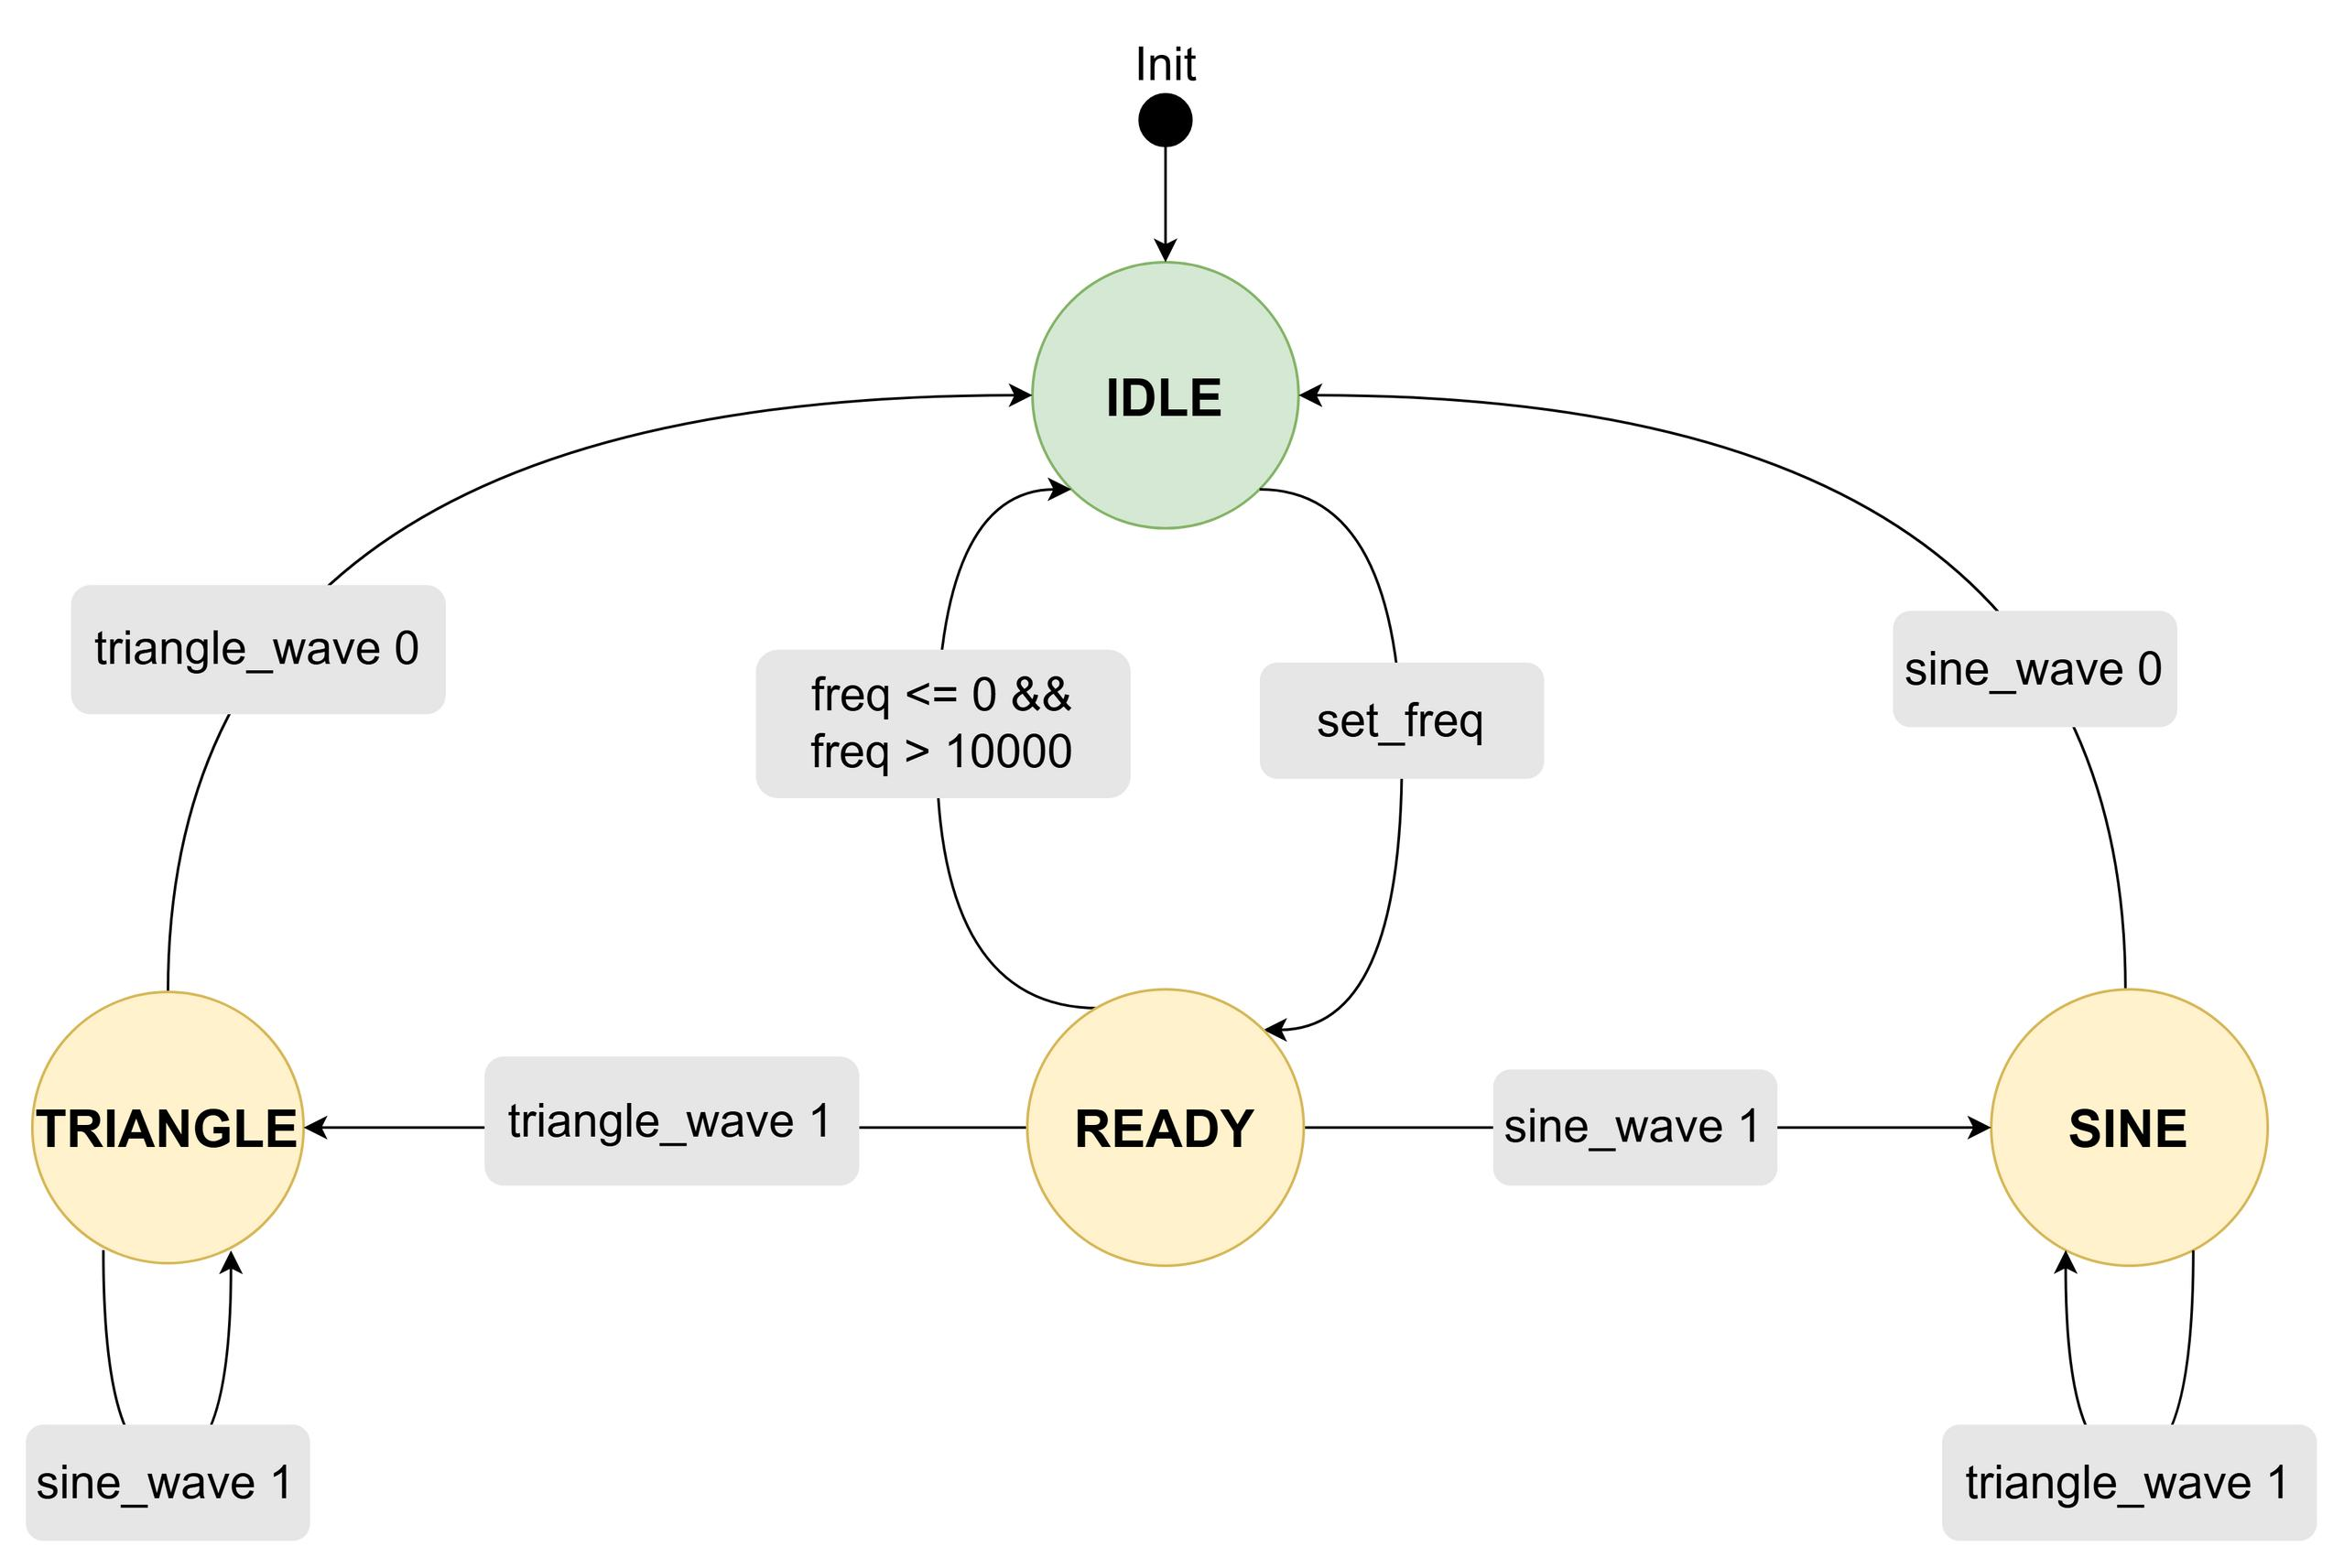
\includegraphics[width=0.8\textwidth]{image/hil_wave.jpg}
    \caption{Sơ đồ máy trạng thái của chức năng tạo sóng}
    \label{fig:hil_wave}
\end{figure}
Chức năng tạo sóng được thiết kế theo sơ đồ máy trạng thái trên với 4 trạng thái chính: \texttt{IDLE} (chờ lệnh cài đặt tần số), \texttt{READY} (chờ lệnh tạo sóng), \texttt{\texttt{SINE}} (tạo sóng sin), \texttt{TRIANGLE} (tạo sóng tam giác).

HIL sẽ cấu hình các ngoại vi cần thiết để thực hiện việc tạo sóng. Trong giai đoạn này, HIL cũng sẽ khởi tạo 2 buffer cho sóng sin và sóng tam giác với số lượng 100 mẫu cho mỗi buffer, công thức cho mỗi dạng sóng sẽ được tính toán ở phần dưới.
Sau giai đoạn khởi tạo, hệ thống sẽ vào trạng thái \texttt{IDLE} để chờ lệnh cấu hình tần số. Khi tần số được cấu hình hợp lệ ($0 < freq \le 10000$), hệ thống chuyển sang trạng thái \texttt{READY} và tính toán tần số cho Timer.
Khi người dùng gửi lệnh bắt đầu tạo sóng sin / tam giác, hệ thống sẽ chuyển sang trạng thái \texttt{SINE} / \texttt{TRIANGLE} tương ứng và bắt đầu tạo sóng. Vì chức năng tạo sóng chỉ được thực hiện bởi 1 phần cứng DAC (PA4) nên tại một thời điểm chỉ có thể tạo được 1 dạng sóng.
Cơ chế này giúp bảo vệ phần cứng không bị xung đột. Cuối cùng, khi có lệnh dừng việc tạo sóng, HIL sẽ trở về trạng thái \texttt{IDLE}.

DAC của STM32F407 có độ phân giải 12 bit, nên giá trị tối đa ($DAC\_MAX$) có thể xuất ra là $2^{12} - 1 = 4095$, tương ứng với mức điện áp 3.3V.

\textbf{Công thức tính toán cho các dạng sóng:}

Đối với sóng sin, biên độ của từng mẫu thứ $i$ (với $i$ chạy từ 0 đến $N-1$) được tính bằng hàm lượng giác và cộng thêm offset để đảm bảo giá trị luôn dương.
\begin{equation}
    V_{sine}[i] = \left( \sin\left(\dfrac{i \cdot 2\pi}{N}\right) + 1 \right) \cdot \dfrac{DAC\_MAX}{2} \cdot 0.98
\end{equation}
Trong đó, hệ số 0.98 được thêm vào nhằm giảm biên độ cực đại chống hiện tượng xén đỉnh.

Đối với sóng tam giác, chu kỳ sóng được chia làm hai nửa đối xứng để tạo độ dốc tuyến tính.
\begin{itemize}
    \item Ở nửa chu kỳ tăng đầu tiên ($i < \dfrac{N}{2}$):
    \begin{equation}
        V_{triangle}[i] = \dfrac{2 \cdot DAC\_MAX \cdot i}{N}
    \end{equation}
    \item Ở nửa chu kỳ giảm tiếp theo ($i \ge \dfrac{N}{2}$):
    \begin{equation}
        V_{triangle}[i] = \dfrac{2 \cdot DAC\_MAX \cdot (N - i)}{N}
    \end{equation}
\end{itemize}

\subsection{Tạo tín hiệu PWM}

\subsection{Xử lý GPIO}


\newpage
\chapter{THIẾT KẾ VÀ THỰC HIỆN PHẦN MỀM NHÚNG CHO LOGIC ANALYZER}

\section{Yêu cầu thiết kế}
Các yêu cầu thiết kế chính cho phần mềm nhúng trên Logic analyzer bao gồm:
\begin{itemize}
    \item Có khả năng giao tiếp USB với máy tính để nhận lệnh cấu hình và điều khiển.
    \item Có khả năng thu thập các tín hiệu số và tín hiệu tương tự từ DUT.
    \item Có tích hợp UART hỗ trợ debug.
\end{itemize}

\section{State machine tổng quát của Logic analyzer}
\begin{figure}[H]
    \centering
    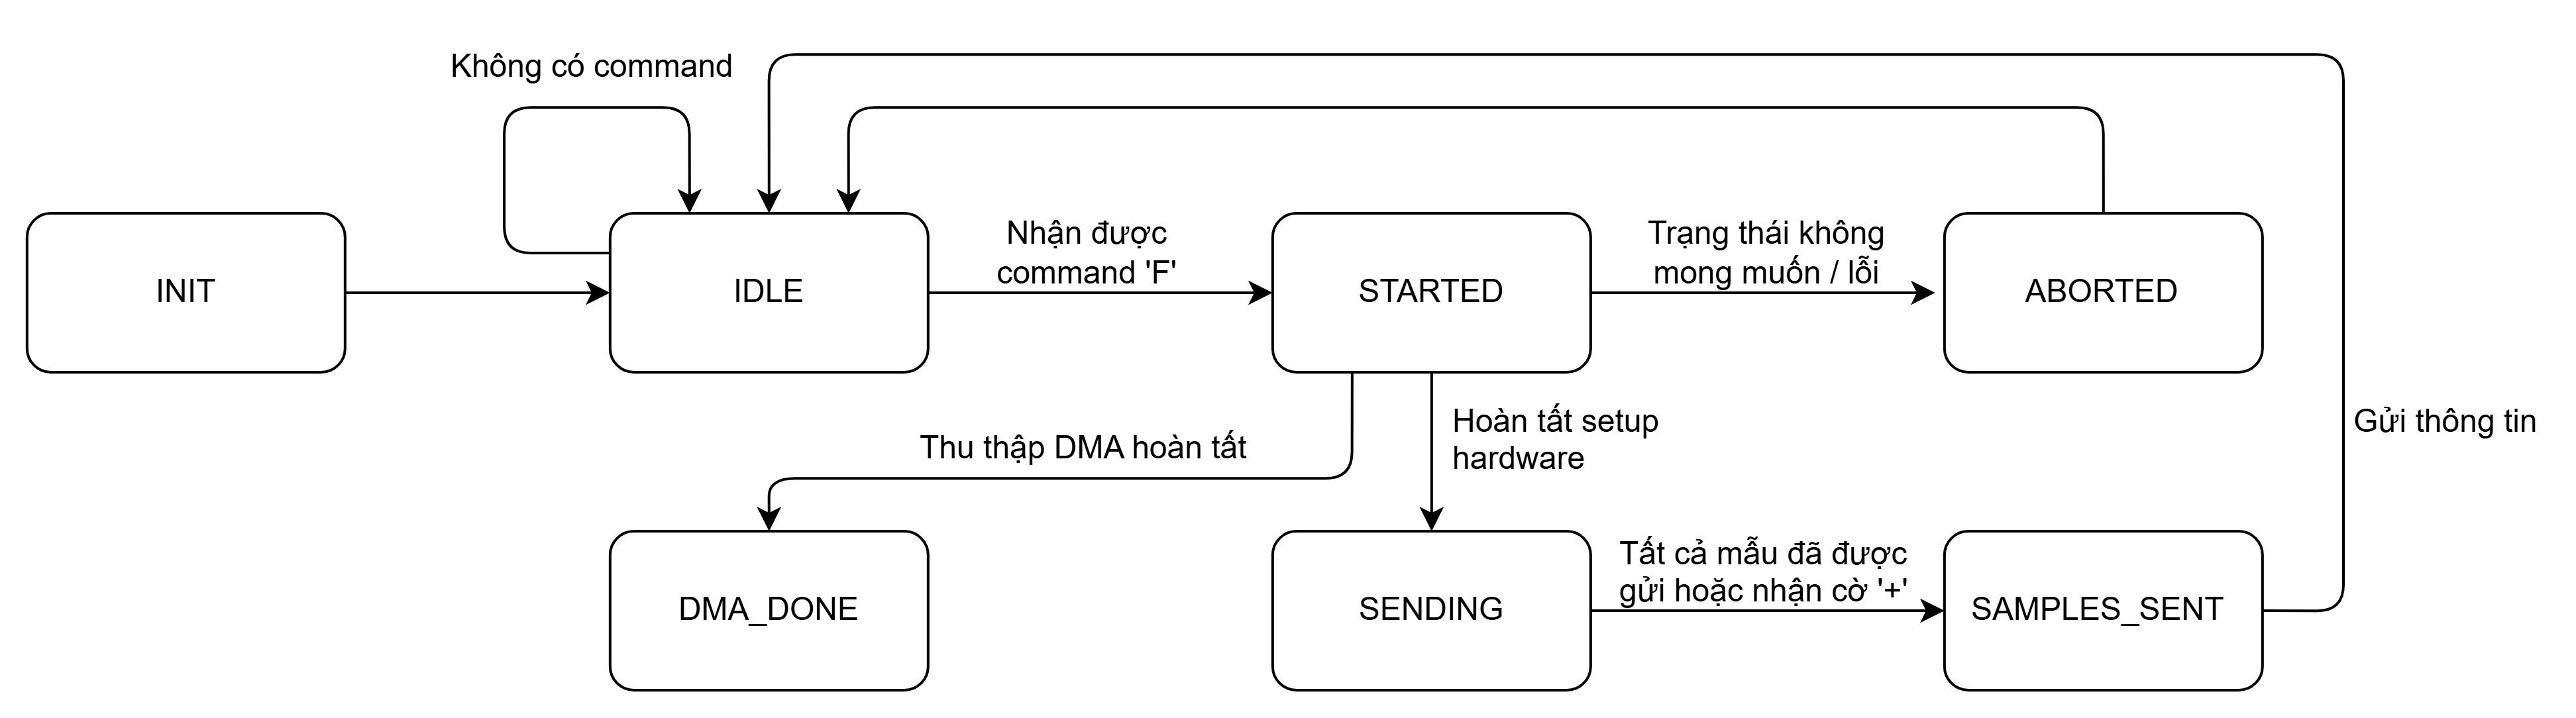
\includegraphics[width=1\textwidth]{image/LA_state_machine.jpg}
    \caption{State machine của Logic analyzer}
    \label{fig:LA_state_machine}
\end{figure}

Các trạng thái chính của Logic analyzer gồm:
\begin{itemize}
    \item \textbf{INIT}: Trạng thái khởi tạo hệ thống, cấu hình các ngoại vi và chuẩn bị cho việc thu thập dữ liệu.
    \item \textbf{IDLE}: Trạng thái chờ lệnh từ máy tính.
    \item \textbf{STARTED}: Trạng thái bắt đầu thu thập dữ liệu.
    \item \textbf{SENDING}: Trạng thái gửi dữ liệu đã thu thập cho máy tính.
    \item \textbf{DMA\_DONE}: Trạng thái hoàn thành thu thập dữ liệu bằng DMA.
    \item \textbf{ABORTED}: Trạng thái hủy bỏ quá trình thu thập dữ liệu do lỗi.
    \item \textbf{SAMPLES\_SENT}: Trạng thái hoàn thành việc gửi dữ liệu.
\end{itemize}

\section{Lưu đồ giải thuật chi tiết của Logic analyzer}
\subsection{Lưu đồ giải thuật của Logic analyzer}
\begin{figure}[H]
    \centering
    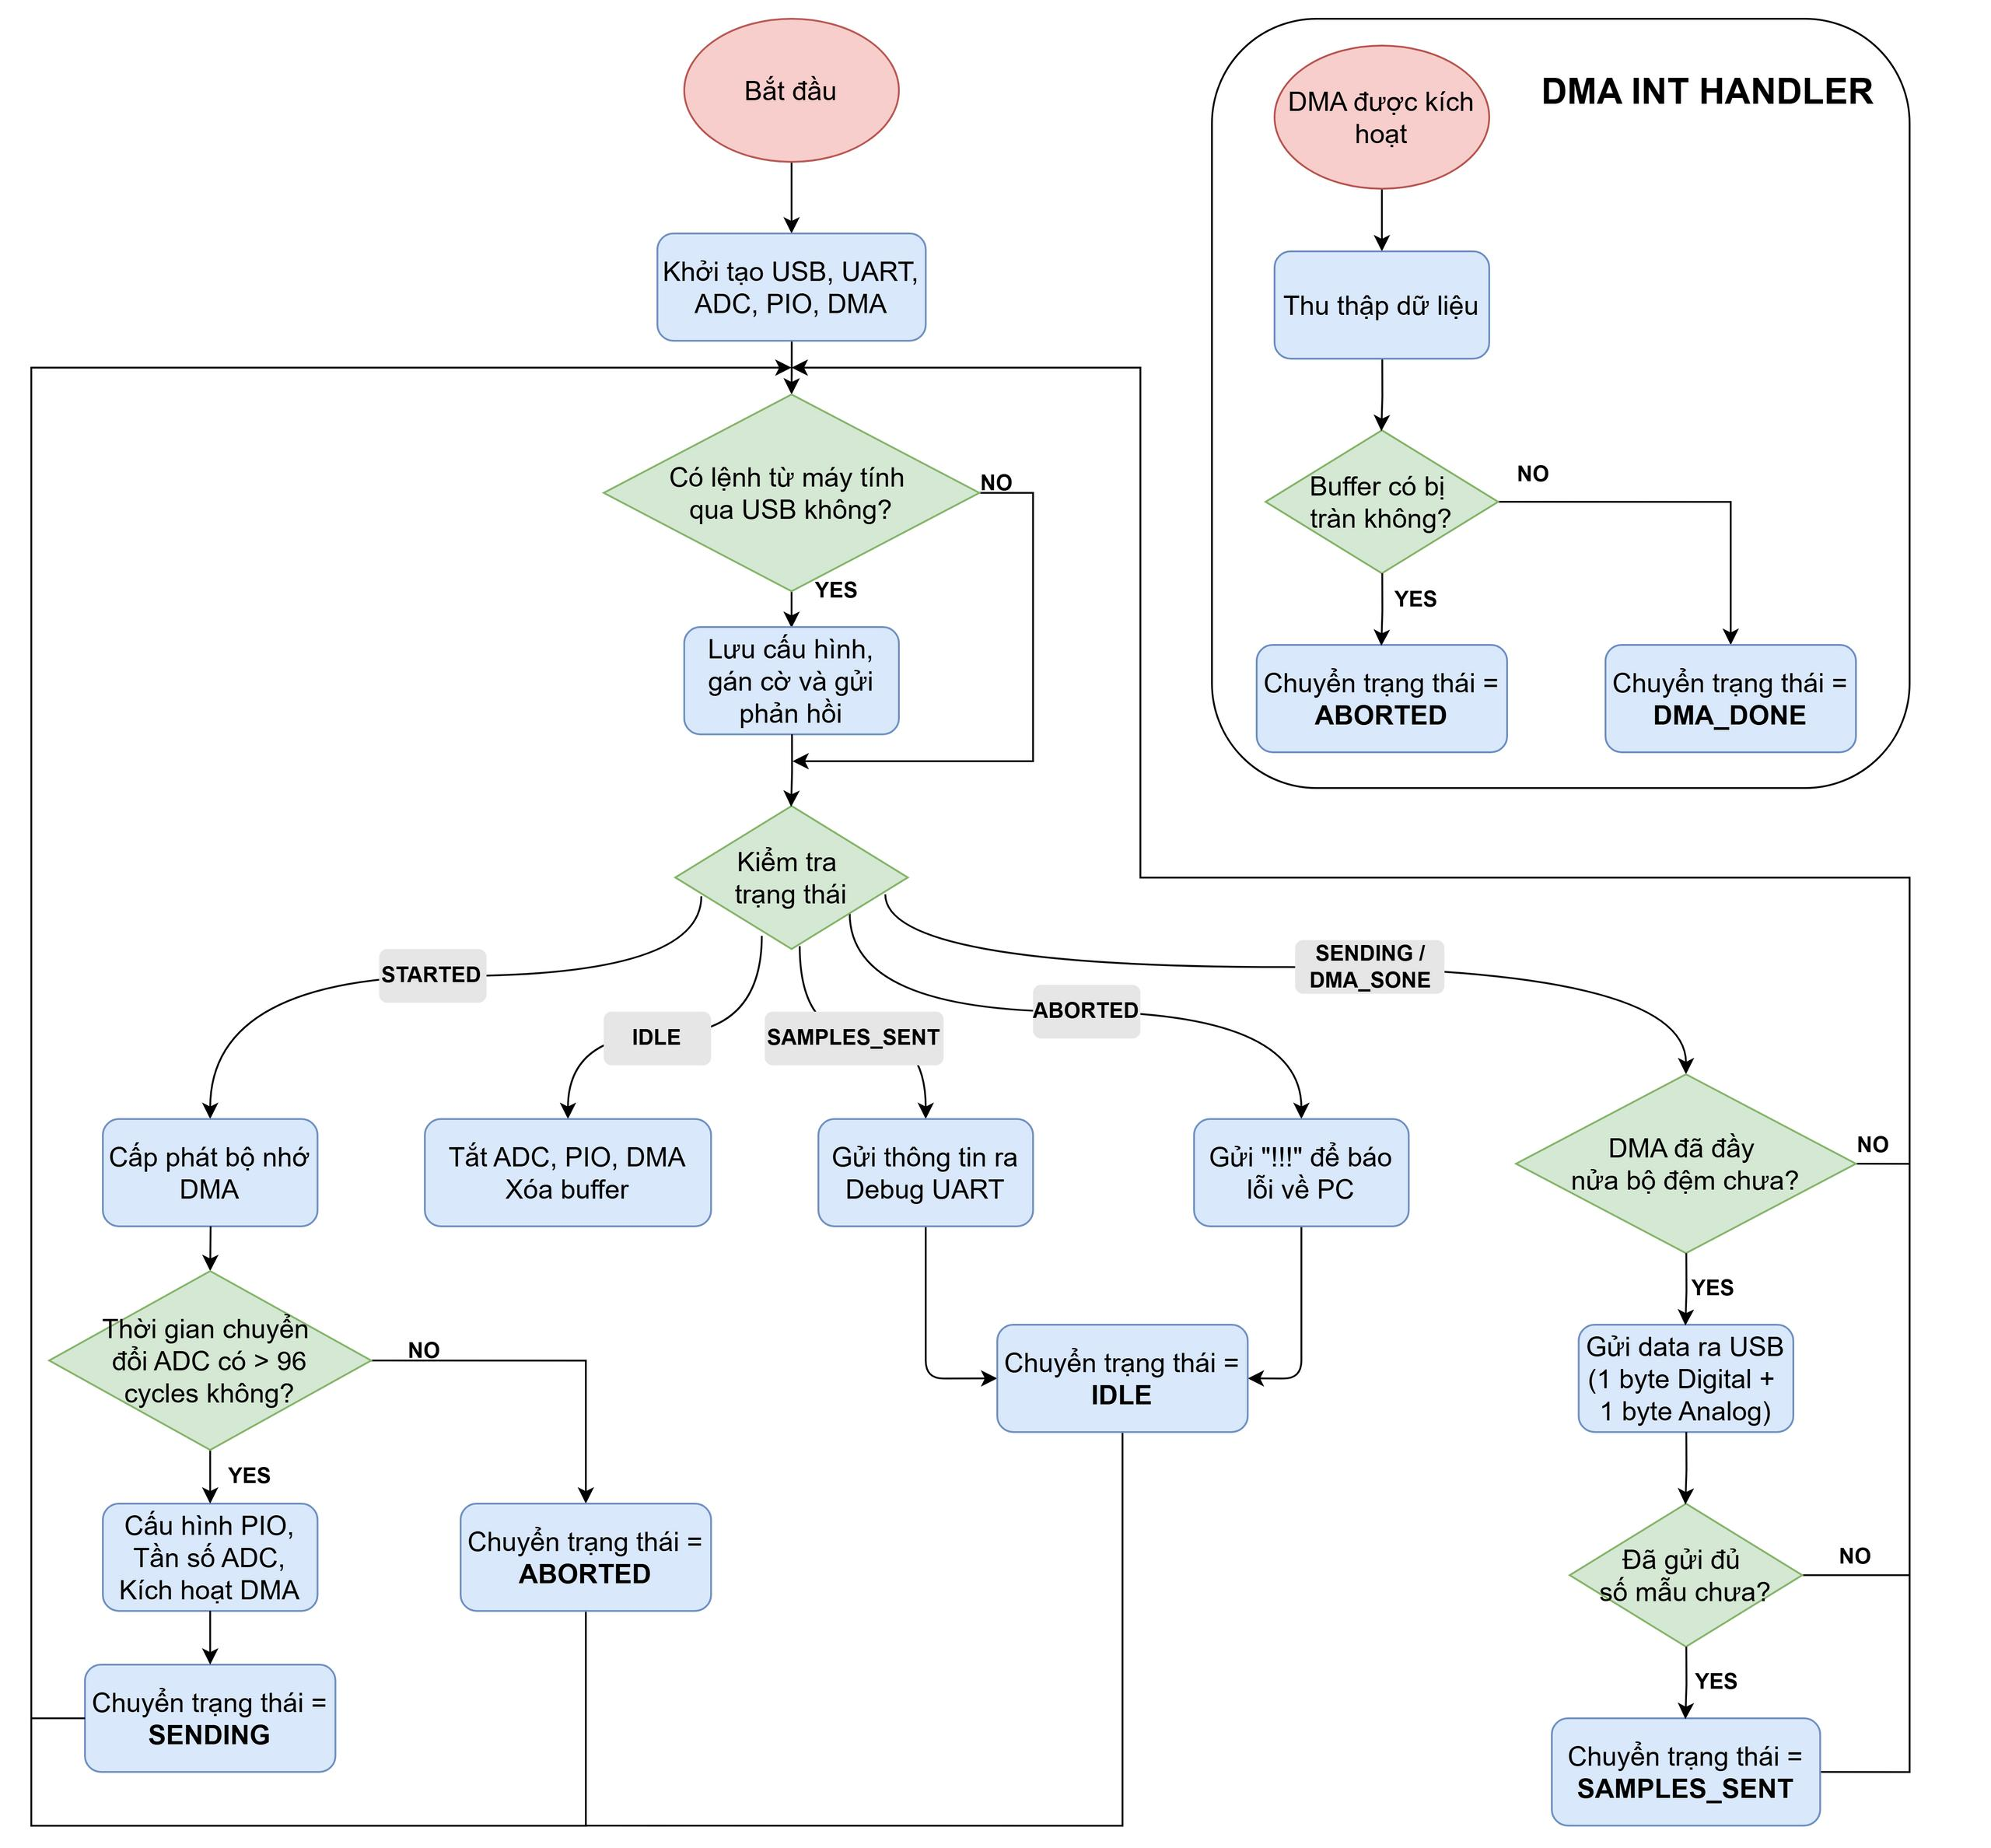
\includegraphics[width=1\textwidth]{image/LA_flow_chart.jpg}
    \caption{Lưu đồ giải thuật của Logic analyzer}
    \label{fig:LA_flow_chart}
\end{figure}

Logic analyzer hoạt động trong một vòng lặp vô hạn kết hợp với ngắt DMA nhằm tối ưu hóa tốc độ cho quá trình thu thập và truyền dữ liệu.
Quá trình bắt đầu bằng việc khởi tạo các ngoại vi cần thiết như USB, UART, ADC, PIO và DMA. Sau khi khởi tạo hoàn tất, hệ thống chuyển sang trạng thái IDLE để chờ lệnh từ máy tính.

Khi nhận được các lệnh từ máy tính, Logic analyzer sẽ lưu cấu hình, gán cờ và gửi phản hồi về máy tính. Nếu nhận được lệnh 'F', Logic analyzer sẽ chuyển sang trạng thái STARTED và thực hiện cấp phát bộ nhớ cho DMA.
Sau đó nếu tính toán nếu thời gian chuyển đổi của ADC lớn hơn 96 cycles, Logic analyzer sẽ tiếp tục cấu hình các ngoại vi khác, kích hoạt DMA và chuyển sang trạng thái SENDING.
Ngược lại, Logic analzyer sẽ chuyển sang trạng thái ABORTED do thời gian chuyển đổi của ADC trên Raspberry Pi tối thiểu là 96 cycles, nếu lấy mẫu với tốc độ quá lớn sẽ dẫn đến các lỗi không mong muốn.

Quá trình gửi và thu thập dữ liệu được thực hiện song song thông qua ngắt DMA (DMA Interrupt Handler). Khi DMA được kích hoạt, dữ liệu sẽ được ghi vào bộ đệm.
Logic analyzer sẽ kiểm tra tình trạng bộ đệm. Nếu không gửi kịp dữ liệu lên máy tính, bộ đệm sẽ bị tràn và hệ thống sẽ chuyển sang trạng thái ABORTED.
Ngược lại, nếu thu thập đủ dữ liệu, Logic analyzer sẽ chuyển sang trạng thái DMA\_DONE.

Trong trạng thái SENDING / DMA\_DONE, Logic analyzer sẽ kiểm tra buffer đã đầy một nửa hay chưa để thực hiện cơ chế truyền dữ liệu theo từng phần.
Dữ liệu sau đó được gửi ra máy tính qua USB, với định dạng mỗi mẫu gồm 1 byte tín hiệu số và 1 byte tín hiệu tương tự. Quá trình này lặp lại cho đến khi toàn bộ số mẫu đã được truyền đi.
Khi đã gửi đủ số mẫu, Logic analyzer sẽ chuyển sang trạng thái SAMPLES\_SENT và tắt ADC, PIO, DMA, xóa bộ đệm để sẵn sàng cho chu kỳ thu thập tiếp theo.

\subsection{Cơ chế xử lý bộ đệm DMA}
\begin{figure}[H]
    \centering
    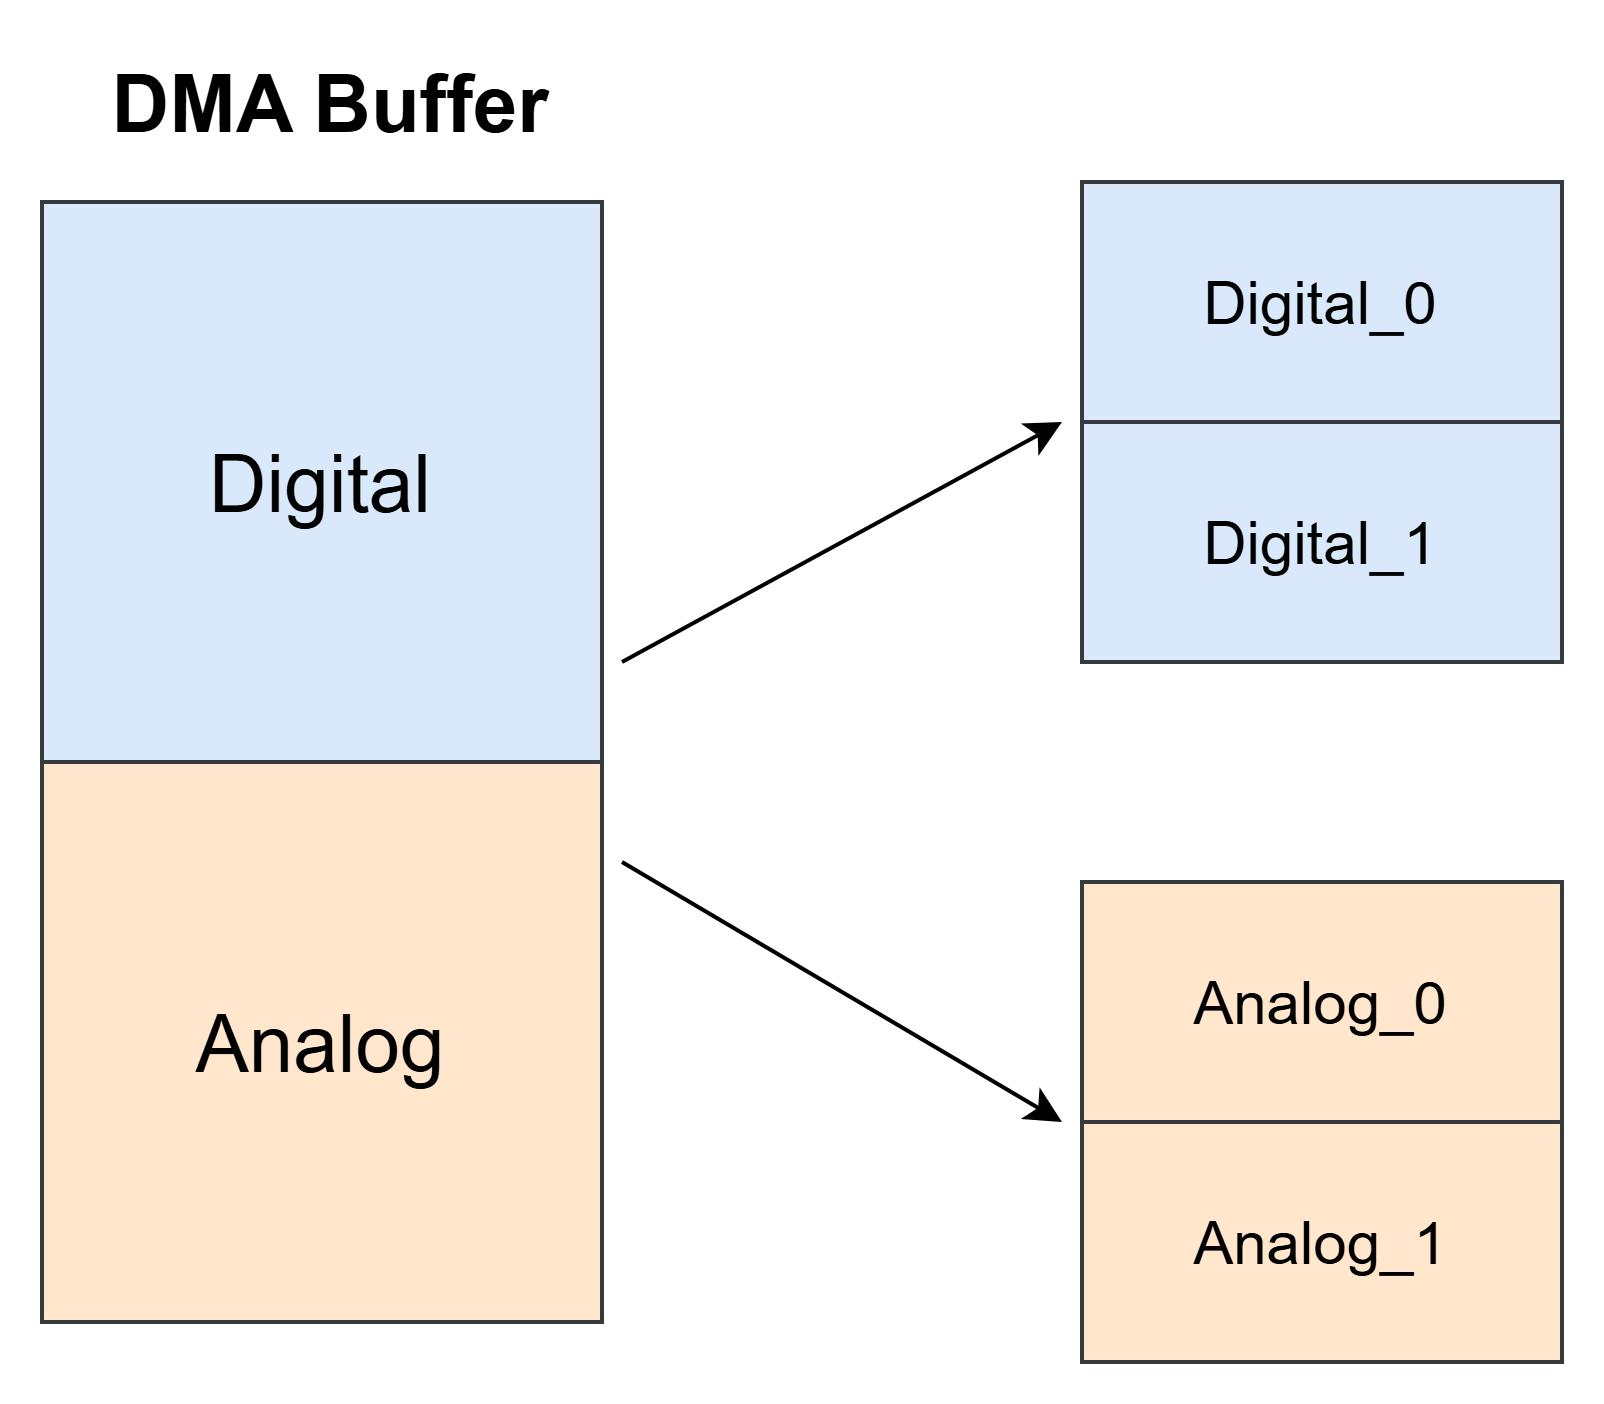
\includegraphics[width=0.5\textwidth]{image/LA_dma_buffer.jpg}
    \caption{Cấp phát bộ đệm DMA}
    \label{fig:LA_dma_buffer}
\end{figure}


\newpage
\input{chuong6}

\newpage
\input{chuong7}

\newpage
\chapter{THIẾT KẾ VÀ THỰC HIỆN HỆ THỐNG KIỂM THỬ TỰ ĐỘNG BẰNG ROBOT FRAMEWORK}
Trong quá trình phát triển hệ thống nhúng, đặc biệt đối với các thiết bị sử dụng nhiều giao tiếp ngoại vi hoặc các cơ chế thời gian thực, việc kiểm thử firmware đóng vai trò rất quan trọng nhằm đảm bảo hệ thống hoạt động đúng chức năng và ổn định trong nhiều điều kiện vận hành khác nhau.

Phương pháp kiểm thử thủ công truyền thống thường yêu cầu người dùng phải trực tiếp gửi lệnh, quan sát tín hiệu phản hồi, so sánh kết quả với giá trị mong đợi và ghi nhận trạng thái hoạt động của hệ thống. Quá trình này không chỉ tốn nhiều thời gian mà còn dễ phát sinh sai sót do yếu tố con người, đặc biệt khi số lượng test case lớn hoặc cần thực hiện kiểm thử lặp lại nhiều lần sau mỗi lần cập nhật firmware. Việc kiểm thử thủ công cũng gây khó khăn trong việc chuẩn hóa quy trình, đảm bảo tính nhất quán giữa các lần kiểm thử và giữa các người dùng khác nhau.

Trong hệ thống hiện tại, phần mềm giao diện được xây dựng bằng PyQt5 chủ yếu phục vụ cho việc cấu hình thiết bị, giám sát trạng thái hoạt động và hỗ trợ thao tác kiểm tra thủ công thông qua giao diện người dùng. Mặc dù phần mềm này có thể hỗ trợ thực hiện một số bài kiểm tra cơ bản, nhưng việc sử dụng giao diện đồ họa để chạy số lượng lớn test case hoặc thực hiện kiểm thử hồi quy thường xuyên vẫn còn nhiều hạn chế. Các thao tác phụ thuộc nhiều vào người vận hành, khó xây dựng quy trình kiểm thử lặp lại hoàn toàn tự động và không thuận lợi cho việc quản lý tập trung các kịch bản kiểm thử.

Đối với hệ thống Hardware-in-the-Loop, việc kiểm thử không chỉ dừng lại ở mức kiểm tra phần mềm mà còn phải đánh giá khả năng tương tác giữa DUT và các thiết bị ngoại vi được mô phỏng bởi hệ thống HIL. Các bài kiểm thử thường bao gồm nhiều bước liên tiếp như cấu hình môi trường mô phỏng, khởi tạo DUT, gửi lệnh điều khiển, thu thập dữ liệu phản hồi và đánh giá kết quả cuối cùng. Nếu thực hiện hoàn toàn thủ công hoặc phụ thuộc chủ yếu vào giao diện điều khiển bằng tay, quá trình này sẽ rất phức tạp, khó đảm bảo tính nhất quán và khó mở rộng khi số lượng bài kiểm thử tăng lên.

Bên cạnh đó, trong quá trình phát triển firmware, mỗi lần thay đổi mã nguồn đều có nguy cơ ảnh hưởng đến các chức năng đã hoạt động ổn định trước đó. Điều này đòi hỏi phải thực hiện kiểm thử hồi quy thường xuyên để phát hiện sớm các lỗi phát sinh ngoài mong muốn. Việc thực hiện kiểm thử hồi quy bằng phương pháp thủ công gần như không khả thi khi hệ thống ngày càng phức tạp, trong khi việc quản lý test case trực tiếp trong phần mềm giao diện cũng không phù hợp cho các quy trình kiểm thử quy mô lớn và lâu dài.

Vì vậy, cần xây dựng một hệ thống kiểm thử tự động độc lập với phần mềm giao diện vận hành, có khả năng tổ chức các test case theo cấu trúc rõ ràng, tự động thực hiện toàn bộ quy trình kiểm thử từ cấu hình hệ thống HIL, điều khiển DUT thực hiện các tác vụ kiểm tra, thu thập dữ liệu phản hồi cho đến đánh giá kết quả PASS/FAIL theo các tiêu chí đã định trước. Hệ thống này giúp giảm đáng kể thời gian kiểm thử, tăng độ chính xác, nâng cao khả năng lặp lại của các bài test và hỗ trợ phát hiện lỗi sớm trong quá trình phát triển sản phẩm.

\section{Lựa chọn Robot Framework cho hệ thống kiểm thử tự động}

Để xây dựng hệ thống kiểm thử tự động cho mô hình Hardware-in-the-Loop, có nhiều phương pháp có thể được lựa chọn như sử dụng Python thuần, unittest, pytest hoặc các công cụ kiểm thử tự động chuyên dụng khác. Mỗi phương pháp đều có những ưu điểm và hạn chế riêng tùy thuộc vào đặc điểm hệ thống cần kiểm thử.

Sử dụng Python thuần cho phép lập trình viên toàn quyền kiểm soát luồng xử lý, dễ dàng xây dựng các hàm giao tiếp phần cứng phức tạp và tối ưu theo từng yêu cầu cụ thể. Tuy nhiên, khi số lượng test case tăng lên, việc quản lý các kịch bản kiểm thử hoàn toàn bằng mã nguồn trở nên khó kiểm soát, khó bảo trì và phụ thuộc nhiều vào kỹ năng lập trình của người viết test. Ngoài ra, việc chuẩn hóa cấu trúc test case, tổ chức báo cáo kết quả và thực hiện kiểm thử hồi quy cũng đòi hỏi phải tự xây dựng thêm nhiều thành phần hỗ trợ.

Các framework như unittest hoặc pytest phù hợp với kiểm thử phần mềm thông thường, đặc biệt là unit test hoặc integration test ở mức hàm và module. Tuy nhiên, đối với hệ thống nhúng có sự tham gia của DUT, HIL và nhiều giao tiếp ngoại vi như UART, I2C, SPI, CAN, việc mô tả các bước kiểm thử theo hướng thao tác thiết bị thực tế sẽ trở nên khó trực quan nếu chỉ sử dụng các framework này. Các test case thường bị gắn chặt với mã nguồn Python, gây khó khăn cho việc theo dõi, bảo trì và mở rộng lâu dài.

Với yêu cầu cần một hệ thống kiểm thử có cấu trúc rõ ràng, dễ quản lý và thuận tiện cho kiểm thử hồi quy, một nền tảng hỗ trợ tổ chức test case theo hướng trực quan và tách biệt với phần xử lý phần cứng là cần thiết. Robot Framework đáp ứng tốt yêu cầu này nhờ hoạt động theo mô hình keyword-driven testing.

Robot Framework là một nền tảng kiểm thử tự động mã nguồn mở hoạt động theo mô hình keyword-driven testing. Trong mô hình này, dữ liệu kiểm thử (Test Data) được xây dựng dưới dạng các test case và keyword mô tả từng bước kiểm tra. Robot Framework đóng vai trò trung tâm điều phối, tiếp nhận các test case này và gọi các thư viện kiểm thử (Test Library) để thực hiện các thao tác thực tế trên hệ thống cần kiểm thử (System Under Test).

Các thư viện kiểm thử có thể là các thư viện có sẵn của Robot Framework hoặc các thư viện Python tự phát triển nhằm phục vụ các yêu cầu đặc thù của hệ thống nhúng như gửi lệnh UART, đọc phản hồi từ DUT, cấu hình môi trường mô phỏng HIL hoặc kiểm tra tín hiệu ngoại vi. Nhờ kiến trúc phân lớp này, phần mô tả test case được tách biệt rõ ràng khỏi phần xử lý giao tiếp phần cứng, giúp hệ thống dễ bảo trì và dễ mở rộng hơn.

\begin{figure}[H]
    \centering
    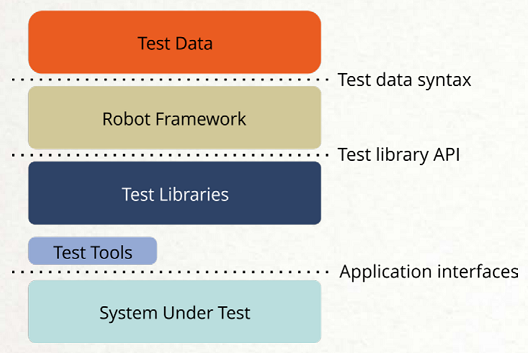
\includegraphics[width=0.85\textwidth]{image/robot_framework_structure.png}
    \caption{Cấu trúc hoạt động của Robot Framework}
    \label{fig:robot_framework_structure}
\end{figure}

Trong phương pháp keyword-driven testing, mỗi thao tác kiểm thử được xây dựng dưới dạng các keyword có ý nghĩa rõ ràng như gửi lệnh, đọc phản hồi, kiểm tra dữ liệu hoặc xác nhận trạng thái hệ thống. Nhờ đó, các test case được biểu diễn dưới dạng các bước kiểm thử trực quan, dễ đọc và gần với quy trình kiểm thử thực tế hơn so với việc viết hoàn toàn bằng mã nguồn Python.

Ưu điểm lớn nhất của Robot Framework là khả năng chuẩn hóa cấu trúc test case và tách biệt rõ ràng giữa phần logic kiểm thử với phần xử lý giao tiếp phần cứng. Các thao tác phức tạp như gửi lệnh UART, cấu hình EEPROM giả lập, điều khiển RTC, đọc dữ liệu Logic Analyzer hoặc kiểm tra tín hiệu PWM có thể được xây dựng trong các thư viện Python tự phát triển, sau đó đóng gói thành các keyword đơn giản để tái sử dụng trong nhiều test case khác nhau. Điều này giúp hệ thống vừa giữ được tính linh hoạt của Python, vừa đảm bảo khả năng quản lý tập trung và dễ bảo trì.

Bên cạnh đó, Robot Framework hỗ trợ tự động sinh báo cáo kiểm thử dưới dạng log, report và thống kê kết quả PASS/FAIL sau mỗi lần thực thi. Đây là một ưu điểm rất quan trọng trong kiểm thử firmware vì giúp kỹ sư dễ dàng theo dõi kết quả, phân tích lỗi và thực hiện kiểm thử hồi quy sau mỗi lần cập nhật firmware mà không cần xây dựng thêm hệ thống báo cáo riêng.

Tuy nhiên, Robot Framework cũng tồn tại một số hạn chế. Đối với các bài kiểm thử có logic xử lý quá phức tạp hoặc yêu cầu kiểm soát rất chi tiết ở mức thấp, việc biểu diễn hoàn toàn bằng keyword có thể trở nên cồng kềnh hơn so với viết trực tiếp bằng Python. Ngoài ra, hiệu năng thực thi của Robot Framework thường không tối ưu bằng chương trình Python thuần trong các tác vụ yêu cầu xử lý tốc độ rất cao. Vì vậy, Robot Framework phù hợp nhất khi được sử dụng như một lớp điều phối kiểm thử, trong khi các thao tác phần cứng phức tạp vẫn được xử lý bởi các thư viện Python chuyên biệt.

Trong phạm vi đề tài này, mục tiêu chính là xây dựng một hệ thống kiểm thử tự động có khả năng tổ chức test case rõ ràng, dễ mở rộng, dễ bảo trì và hỗ trợ kiểm thử hồi quy lâu dài cho hệ thống HIL. Do đó, Robot Framework là lựa chọn phù hợp hơn so với Python thuần hoặc các framework kiểm thử thông thường. Việc kết hợp Robot Framework với các thư viện Python tự phát triển giúp tận dụng được ưu điểm của cả hai phương pháp, vừa đảm bảo khả năng kiểm soát giao tiếp phần cứng, vừa xây dựng được một hệ thống kiểm thử chuyên nghiệp, có khả năng mở rộng trong tương lai.

\section{Yêu cầu thiết kế}

Hệ thống kiểm thử tự động được xây dựng nhằm hỗ trợ kiểm thử firmware của DUT trong môi trường Hardware-in-the-Loop một cách chính xác, ổn định và có khả năng mở rộng. Để đáp ứng yêu cầu này, hệ thống cần thỏa mãn các tiêu chí thiết kế sau:

\begin{itemize}

    \item Hệ thống phải cung cấp một thư viện các hàm kiểm thử chuyên biệt để giao tiếp với DUT và HIL, bao gồm các thao tác như gửi lệnh điều khiển, đọc dữ liệu phản hồi, cấu hình môi trường mô phỏng và đánh giá kết quả kiểm thử.

    \item Kiến trúc hệ thống phải đảm bảo tính mở rộng và khả năng bảo trì lâu dài, cho phép dễ dàng bổ sung thư viện mới, xây dựng thêm các kịch bản kiểm thử và cập nhật khi có thay đổi về phần cứng hoặc yêu cầu kiểm thử mới trong quá trình phát triển firmware.

    \item Các kịch bản kiểm thử phải được tổ chức theo cấu trúc rõ ràng, dễ đọc, dễ hiểu và có khả năng tái sử dụng cao, giúp thuận tiện cho việc quản lý, kiểm tra và mở rộng hệ thống kiểm thử trong tương lai.

    \item Hệ thống cần hỗ trợ giao tiếp đồng thời với DUT và hệ thống HIL thông qua các giao tiếp như USB hoặc UART, đảm bảo khả năng điều khiển thiết bị và thu thập dữ liệu phản hồi theo thời gian thực.

    \item Hệ thống phải hỗ trợ cơ chế đánh giá kết quả kiểm thử tự động theo tiêu chí PASS/FAIL dựa trên các giá trị mong đợi đã được định nghĩa trước, hạn chế tối đa sự can thiệp thủ công của người vận hành.

    \item Toàn bộ dữ liệu kiểm thử bao gồm lệnh điều khiển, phản hồi từ DUT, trạng thái của HIL và kết quả đánh giá cần được ghi nhận đầy đủ nhằm phục vụ việc phân tích lỗi, debug firmware và truy vết kết quả kiểm thử.

    \item Hệ thống phải hỗ trợ thực hiện kiểm thử đồng thời nhiều test case, cho phép chạy các kịch bản kiểm thử liên tiếp hoặc song song để tối ưu hóa thời gian kiểm thử, đặc biệt trong các tình huống cần thực hiện kiểm thử hồi quy sau mỗi lần cập nhật firmware.

\end{itemize}

Cấu trúc triển khai cụ thể của hệ thống kiểm thử tự động trong môi trường Hardware-in-the-Loop được trình bày trong Hình \ref{fig:hil_robot_structure}.

\begin{figure}[H]
    \centering
    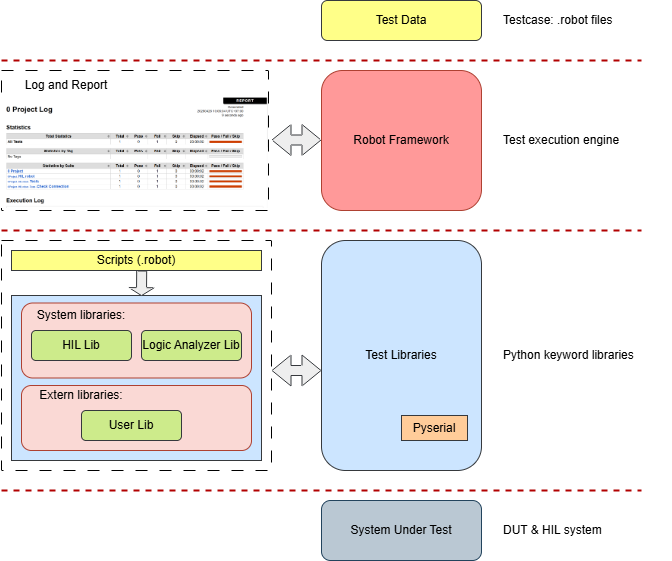
\includegraphics[width=0.85\textwidth]{image/hil_robot_structure.png}
    \caption{Cấu trúc triển khai Robot Framework trong hệ thống HIL}
    \label{fig:hil_robot_structure}
\end{figure}

Khác với cấu trúc tổng quan của Robot Framework đã trình bày ở phần trước, hình \ref{fig:hil_robot_structure} mô tả cách hệ thống kiểm thử được triển khai cụ thể trong phạm vi đề tài.

Các test case được xây dựng dưới dạng các file \texttt{.robot}, trong đó mỗi bài kiểm thử tương ứng với một chức năng ngoại vi như GPIO, PWM, UART, I2C, SPI hoặc CAN. Mỗi test case bao gồm các bước cấu hình môi trường kiểm thử, điều khiển DUT thực hiện tác vụ cần kiểm tra, thu thập dữ liệu phản hồi và đánh giá kết quả cuối cùng.

Robot Framework đóng vai trò điều phối trung tâm, thực thi tuần tự các test case và gọi các keyword tương ứng trong các thư viện kiểm thử. Đối với hệ thống HIL và Logic Analyzer, các keyword được xây dựng sẵn và lưu trữ trong thư viện hệ thống. Các keyword này tương ứng trực tiếp với toàn bộ tập lệnh được hỗ trợ bởi HIL và Logic Analyzer, cho phép thực hiện các thao tác gửi lệnh, nhận phản hồi và cấu hình môi trường mô phỏng. Bên cạnh đó, hệ thống cũng cung cấp thêm các keyword tiện ích phục vụ kiểm thử như kiểm tra trạng thái thiết bị, so sánh giá trị phản hồi với giá trị mong đợi và xác nhận kết quả PASS/FAIL.

Đối với DUT, thư viện kiểm thử được xây dựng riêng tùy theo từng thiết bị cần kiểm tra, dựa trên tập lệnh và yêu cầu chức năng cụ thể của firmware và sẽ do người dùng xây dựng. Cách tổ chức này giúp hệ thống có tính linh hoạt cao, dễ dàng mở rộng cho nhiều loại DUT khác nhau mà không ảnh hưởng đến kiến trúc tổng thể của hệ thống kiểm thử.

Tầng giao tiếp vật lý sử dụng thư viện \texttt{pyserial} để kết nối với DUT, HIL và Logic Analyzer thông qua cổng USB serial. Thư viện này chịu trách nhiệm thực hiện truyền nhận dữ liệu, đồng bộ quá trình kiểm thử và đảm bảo luồng giao tiếp ổn định giữa các thiết bị trong suốt quá trình thực thi test case.

Sau khi quá trình kiểm thử hoàn tất, Robot Framework tự động sinh ra các tệp báo cáo như \texttt{report.html}, \texttt{log.html} và \texttt{output.xml}. Trong đó, \texttt{report.html} cung cấp kết quả tổng quan của toàn bộ quá trình kiểm thử với trạng thái PASS/FAIL của từng test case, \texttt{log.html} ghi lại chi tiết từng bước thực thi, các lệnh đã gửi, dữ liệu phản hồi và thông tin debug trong quá trình kiểm thử, còn \texttt{output.xml} được sử dụng để lưu trữ dữ liệu kết quả dưới dạng có cấu trúc phục vụ cho việc phân tích hoặc tích hợp với các hệ thống kiểm thử khác. Việc tự động ghi nhận log và sinh báo cáo giúp kỹ sư dễ dàng truy vết lỗi, đánh giá chất lượng firmware và thực hiện kiểm thử hồi quy một cách hiệu quả.

Nhờ cấu trúc phân lớp này, hệ thống kiểm thử vừa đảm bảo tính tự động hóa cao, vừa dễ dàng mở rộng khi cần bổ sung thêm ngoại vi mới hoặc xây dựng thêm các bài kiểm thử trong tương lai.


\section{Thiết kế các kịch bản kiểm thử}

Dựa trên kiến trúc hệ thống kiểm thử đã xây dựng cùng tập các keyword hỗ trợ cho HIL và Logic Analyzer, bước tiếp theo là thiết kế các kịch bản kiểm thử cụ thể cho từng chức năng ngoại vi của DUT. Các keyword được sử dụng như những khối chức năng cơ bản để xây dựng quy trình kiểm thử hoàn chỉnh, bao gồm thiết lập môi trường kiểm thử, điều khiển DUT và HIL, thu thập dữ liệu phản hồi cũng như đánh giá kết quả theo tiêu chí PASS/FAIL.

Mỗi kịch bản kiểm thử được xây dựng nhằm xác minh tính đúng đắn của firmware khi thực hiện giao tiếp với các thiết bị ngoại vi được mô phỏng bởi hệ thống HIL.

Phần tiếp theo trình bày lưu đồ giải thuật chi tiết của một số nhóm test case tiêu biểu được triển khai trong đề tài.

\subsection{Kiểm tra kết nối của HIL và DUT}

Mục đích của bài kiểm thử này là xác minh khả năng kết nối và giao tiếp giữa PC với HIL, đồng thời giữa PC với DUT, nhằm đảm bảo toàn bộ hệ thống sẵn sàng cho các bài kiểm thử chức năng tiếp theo.

Quy trình kiểm thử bao gồm các bước sau:

\begin{itemize}
    \item Bước 1: Kết nối HIL với PC thông qua cổng USB serial và kiểm tra khả năng nhận diện thiết bị.
    \item Bước 2: Cấp nguồn cho DUT thông qua hệ thống HIL để chuẩn bị cho quá trình kiểm thử.
    \item Bước 3: Kết nối DUT với PC thông qua cổng USB hoặc UART và xác nhận thiết bị có thể giao tiếp.
    \item Bước 4: Gửi lệnh kiểm tra cơ bản từ PC đến HIL và DUT, thu thập phản hồi để xác minh khả năng giao tiếp hai chiều.
    \item Bước 5: Đánh giá kết quả kiểm thử dựa trên phản hồi nhận được.
\end{itemize}

Điều kiện đánh giá:

\begin{itemize}
    \item PASS: HIL và DUT đều được nhận diện đúng, có thể giao tiếp và phản hồi chính xác lệnh kiểm tra.
    \item FAIL: Ít nhất một trong hai thiết bị không được nhận diện, không thể giao tiếp hoặc phản hồi không chính xác.
\end{itemize}

Lưu đồ giải thuật tổng quát của bài kiểm thử được trình bày trong Hình \ref{fig:connection_test_flowchart}.

\begin{figure}[H]
    \centering
    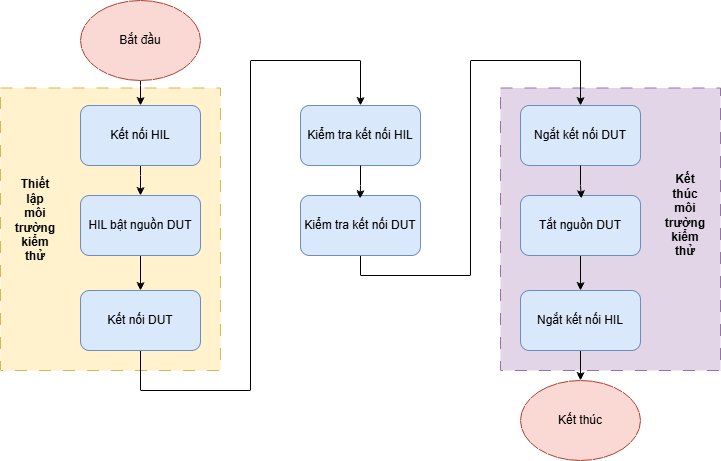
\includegraphics[width=0.8\textwidth]{image/connection_test_flowchart.png}
    \caption{Lưu đồ giải thuật kiểm tra kết nối HIL và DUT}
    \label{fig:connection_test_flowchart}
\end{figure}

Đây là bài kiểm thử cơ bản nhất nhằm đảm bảo hệ thống đã được thiết lập đúng trước khi thực hiện các bài kiểm thử chức năng khác. Trong đó, ba bước đầu gồm kết nối HIL, cấp nguồn cho DUT và kết nối DUT sẽ được quy ước là giai đoạn thiết lập môi trường kiểm thử. Tương tự, các bước ngắt kết nối DUT, tắt nguồn DUT và ngắt kết nối HIL ở cuối quá trình được quy ước là giai đoạn kết thúc môi trường kiểm thử.

Giữa hai giai đoạn này là phần kiểm thử chính, được thay đổi tùy theo yêu cầu của từng test case cụ thể. Đối với bài kiểm tra kết nối, thao tác chính là gửi lệnh kiểm tra cơ bản như \texttt{help} đến HIL và DUT, sau đó thu thập phản hồi và so sánh với giá trị mong đợi để xác minh trạng thái hoạt động của thiết bị.

Lưu đồ giải thuật chi tiết cho quá trình xác minh kết nối được trình bày trong Hình \ref{fig:verify_connection_flowchart}.

\begin{figure}[H]
    \centering
    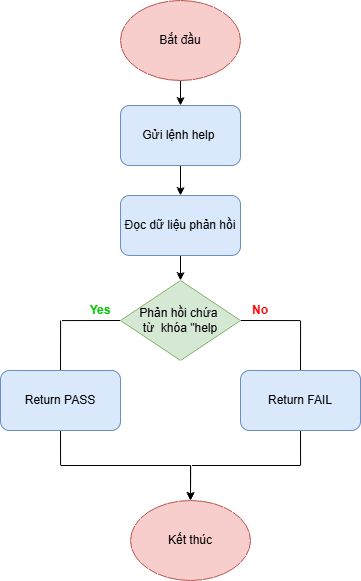
\includegraphics[height=0.4\textheight]{image/verify_connection_flowchart.png}
    \caption{Lưu đồ giải thuật xác minh kết nối của HIL và DUT với PC}
    \label{fig:verify_connection_flowchart}
\end{figure}

\subsection{Kiểm tra khả năng flash firmware cho DUT}

Mục đích của bài kiểm thử này là xác minh khả năng nạp firmware mới cho DUT thông qua hệ thống HIL, đảm bảo quá trình cập nhật chương trình được thực hiện đúng, ổn định và DUT có thể khởi động lại với firmware mới sau khi hoàn tất.

Quy trình kiểm thử bao gồm các bước sau:

\begin{itemize}
    \item Bước 1: Kiểm tra kết nối giữa PC, HIL và DUT, đảm bảo hệ thống sẵn sàng cho quá trình nạp firmware.
    \item Bước 2: Tắt nguồn DUT và điều khiển chân BOOT0 ở mức cao thông qua HIL để đưa DUT vào chế độ DFU (Device Firmware Upgrade).
    \item Bước 3: Cấp nguồn lại cho DUT và kiểm tra việc nhận diện thiết bị DFU trên máy tính.
    \item Bước 4: Sử dụng công cụ STM32CubeProgrammer CLI để thực hiện nạp firmware vào bộ nhớ Flash của DUT.
    \item Bước 5: Sau khi nạp hoàn tất, đưa chân BOOT0 về mức thấp và khởi động lại DUT để chạy chương trình mới.
    \item Bước 6: Kiểm tra phản hồi từ DUT nhằm xác minh firmware đã được nạp thành công và hệ thống hoạt động bình thường.
\end{itemize}

Điều kiện đánh giá:

\begin{itemize}
    \item PASS: DUT được nhận diện đúng ở chế độ DFU, firmware được nạp thành công, xác minh Flash hợp lệ và DUT khởi động lại bình thường với chương trình mới.
    \item FAIL: Bài kiểm thử sẽ trả về FAILD nếu gặp bất kì lỗi nào sau đây: DUT không vào được chế độ DFU, quá trình nạp firmware thất bại, xác minh Flash lỗi hoặc DUT không hoạt động đúng sau khi khởi động lại.
\end{itemize}

Lưu đồ giải thuật tổng quát của bài kiểm thử được trình bày trong Hình \ref{fig:flash_fw_flowchart}.

\begin{figure}[H]
    \centering
    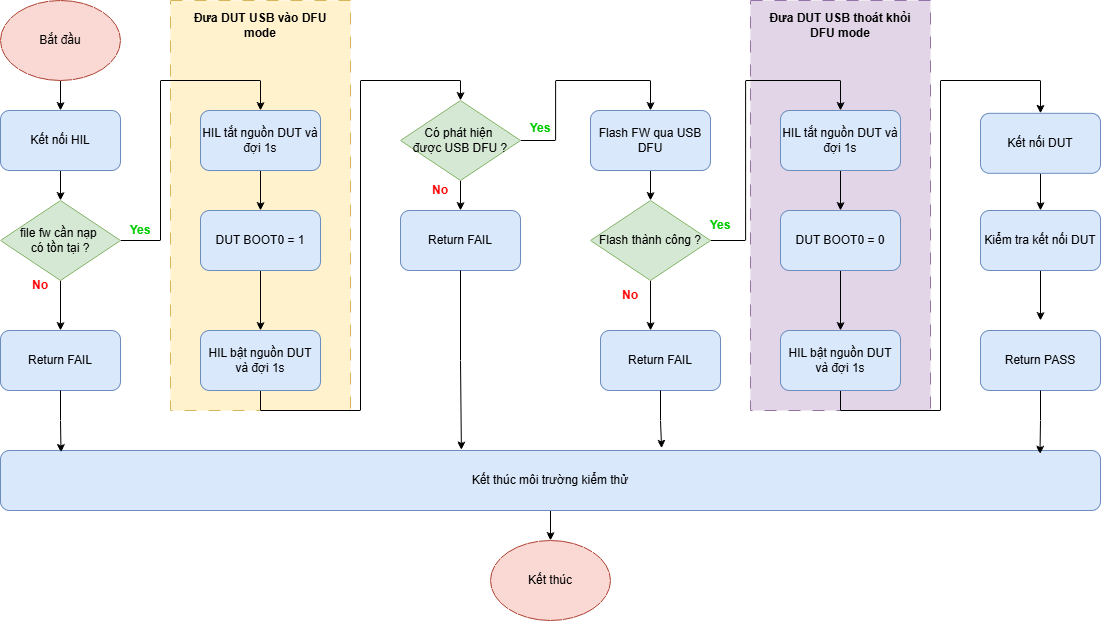
\includegraphics[width=0.8\textwidth]{image/flash_fw_flowchart.png}
    \caption{Lưu đồ giải thuật kiểm tra khả năng flash firmware cho DUT}
    \label{fig:flash_fw_flowchart}
\end{figure}

Trong bài kiểm thử này, hệ thống HIL đóng vai trò hỗ trợ điều khiển phần cứng của DUT, bao gồm bật/tắt nguồn và điều khiển chân BOOT0 để chuyển DUT vào chế độ bootloader. Sau đó, Robot Framework sử dụng thư viện Python để gọi công cụ STM32CubeProgrammer CLI thực hiện quá trình nạp firmware tự động.

Sau khi hoàn tất quá trình ghi Flash, DUT được đưa trở lại chế độ hoạt động bình thường bằng cách đưa BOOT0 về mức thấp và thực hiện reset nguồn. Bước cuối cùng là xác minh DUT có thể khởi động thành công với firmware mới, đảm bảo toàn bộ quá trình cập nhật chương trình diễn ra chính xác và ổn định.

\subsection{Kiểm tra ngoại vi GPIO}
Mục đích của bài kiểm thử này là xác minh khả năng điều khiển và phản hồi tín hiệu GPIO của DUT ở cả hai chế độ GPIO Output và GPIO Input. Bài kiểm thử nhằm đảm bảo firmware cấu hình đúng chế độ hoạt động của chân GPIO, đồng thời tín hiệu thực tế tại chân vi điều khiển phù hợp với trạng thái mong đợi trong từng trường hợp kiểm thử.

Đối với GPIO Output, DUT chủ động xuất mức logic ra các chân điều khiển LED và hệ thống HIL thực hiện giám sát trạng thái tín hiệu thực tế tại các chân này. Đối với GPIO Input, HIL đóng vai trò tạo tín hiệu mức logic đầu vào, trong khi DUT thực hiện đọc trạng thái chân GPIO và phản hồi kết quả về PC để xác minh tính đúng đắn của quá trình nhận tín hiệu.

Quy trình kiểm thử tổng quát bao gồm các bước sau:

\begin{itemize}
    \item Bước 1: Thiết lập môi trường kiểm thử bằng cách kết nối HIL, cấp nguồn cho DUT và thiết lập kết nối với DUT.
    \item Bước 2: Thực hiện bài kiểm thử GPIO Output, trong đó DUT điều khiển trạng thái các chân GPIO đầu ra và HIL kiểm tra mức logic thực tế tại các chân tương ứng.
    \item Bước 3: Thực hiện bài kiểm thử GPIO Input, trong đó HIL tạo tín hiệu mức logic đầu vào và DUT đọc trạng thái các chân GPIO để xác minh kết quả nhận được.
    \item Bước 4: Đánh giá kết quả kiểm thử dựa trên toàn bộ phản hồi thu được từ cả hai bài kiểm thử.
    \item Bước 5: Kết thúc môi trường kiểm thử bằng cách ngắt kết nối DUT, tắt nguồn DUT và ngắt kết nối HIL.
\end{itemize}

Điều kiện đánh giá:

\begin{itemize}
    \item PASS: Tất cả các chân GPIO ở cả hai chế độ Output và Input đều hoạt động đúng, tín hiệu đọc được từ HIL và DUT khớp với giá trị mong đợi.
    \item FAIL: Có ít nhất một chân GPIO không thay đổi đúng trạng thái hoặc giá trị đọc được không khớp với trạng thái mong đợi.
\end{itemize}

Lưu đồ giải thuật tổng quát của bài kiểm thử được trình bày trong Hình \ref{fig:gpio_test_flowchart}.

\begin{figure}[H]
    \centering
    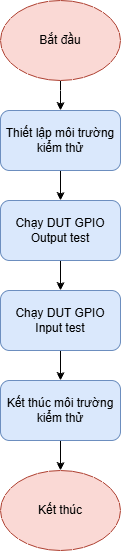
\includegraphics[height=0.4\textheight]{image/gpio_test_flowchart.png}
    \caption{Lưu đồ giải thuật tổng quát kiểm tra chức năng GPIO}
    \label{fig:gpio_test_flowchart}
\end{figure}

Trong bài kiểm thử GPIO Output, DUT đóng vai trò chủ động điều khiển trạng thái logic các chân GPIO. Hệ thống HIL sẽ đọc trực tiếp mức logic tại các chân này và so sánh với giá trị mong đợi để xác minh tính chính xác của tín hiệu đầu ra.

Lưu đồ giải thuật chi tiết của phần kiểm thử GPIO Output được trình bày trong Hình \ref{fig:gpio_output_test_flowchart}.

\begin{figure}[H]
    \centering
    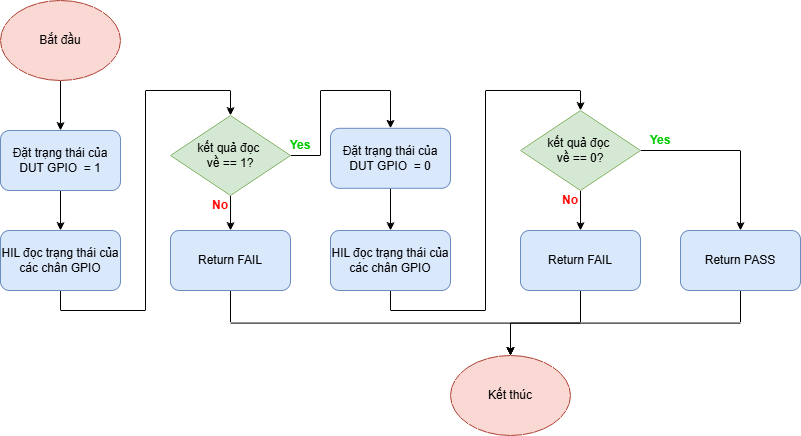
\includegraphics[width=0.8\textwidth]{image/gpio_output_test_flowchart.png}
    \caption{Lưu đồ giải thuật kiểm tra GPIO Output}
    \label{fig:gpio_output_test_flowchart}
\end{figure}

Trong bài kiểm thử GPIO Input, vai trò giữa DUT và HIL được thực hiện theo hướng ngược lại. HIL đóng vai trò chủ động điều khiển trạng thái logic các chân GPIO. DUT sẽ đọc trực tiếp mức logic tại các chân này và so sánh với giá trị mong đợi để xác minh tính chính xác của tín hiệu đầu ra.

Lưu đồ giải thuật chi tiết của phần kiểm thử GPIO Input được trình bày trong Hình \ref{fig:gpio_input_test_flowchart}.

\begin{figure}[H]
    \centering
    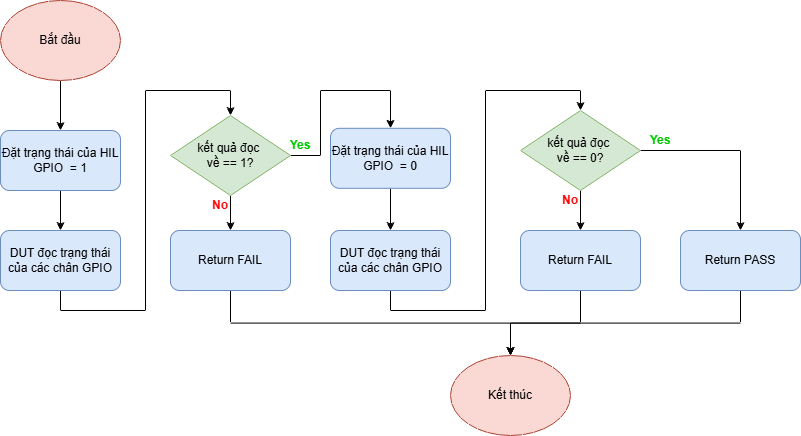
\includegraphics[width=0.8\textwidth]{image/gpio_input_test_flowchart.png}
    \caption{Lưu đồ giải thuật kiểm tra GPIO Input}
    \label{fig:gpio_input_test_flowchart}
\end{figure}

\subsection{Kiểm tra ngoại vi ADC}

Mục đích của bài kiểm thử này là xác minh khả năng đọc tín hiệu analog của DUT thông qua bộ chuyển đổi tương tự sang số. Bài kiểm thử nhằm đảm bảo firmware cần kiểm thử cấu hình đúng chức năng ADC, đồng thời giá trị điện áp đo được từ DUT phản ánh chính xác tín hiệu đầu vào do hệ thống HIL cung cấp.

Trong bài kiểm thử này, hệ thống HIL đóng vai trò tạo tín hiệu điện áp analog đầu vào thông qua ngõ ra DAC với các mức điện áp xác định trước. DUT thực hiện đọc giá trị điện áp tại chân ADC, sau đó phản hồi kết quả đo về PC để tiến hành so sánh với giá trị mong đợi.

Quy trình kiểm thử tổng quát bao gồm các bước sau:

\begin{itemize}
    \item Bước 1: Thiết lập môi trường kiểm thử bằng cách kết nối HIL, cấp nguồn cho DUT và thiết lập kết nối với DUT.
    \item Bước 2: Hệ thống HIL lần lượt thiết lập các mức điện áp đầu ra DAC tương ứng với các giá trị kiểm thử: 1.5V, 2.0V, 3.0V và 3.3V.
    \item Bước 3: Sau mỗi lần thiết lập điện áp, DUT thực hiện đọc giá trị ADC tại chân đầu vào tương ứng.
    \item Bước 4: DUT gửi kết quả đo được về PC, hệ thống tiến hành so sánh với giá trị điện áp mong đợi trong khoảng sai số cho phép.
    \item Bước 5: Đánh giá kết quả kiểm thử dựa trên toàn bộ phản hồi thu được.
    \item Bước 6: Kết thúc môi trường kiểm thử bằng cách ngắt kết nối DUT, tắt nguồn DUT và ngắt kết nối HIL.
\end{itemize}

Điều kiện đánh giá:

\begin{itemize}
    \item PASS: Tất cả các giá trị điện áp đo được từ DUT nằm trong khoảng sai số cho phép so với giá trị điện áp đầu vào do HIL cung cấp.
    \item FAIL: Có ít nhất một giá trị đo không nằm trong khoảng sai số cho phép hoặc DUT không phản hồi kết quả đo.
\end{itemize}

Lưu đồ giải thuật tổng quát của bài kiểm thử được trình bày trong Hình \ref{fig:adc_test_flowchart}.

\begin{figure}[H]
    \centering
    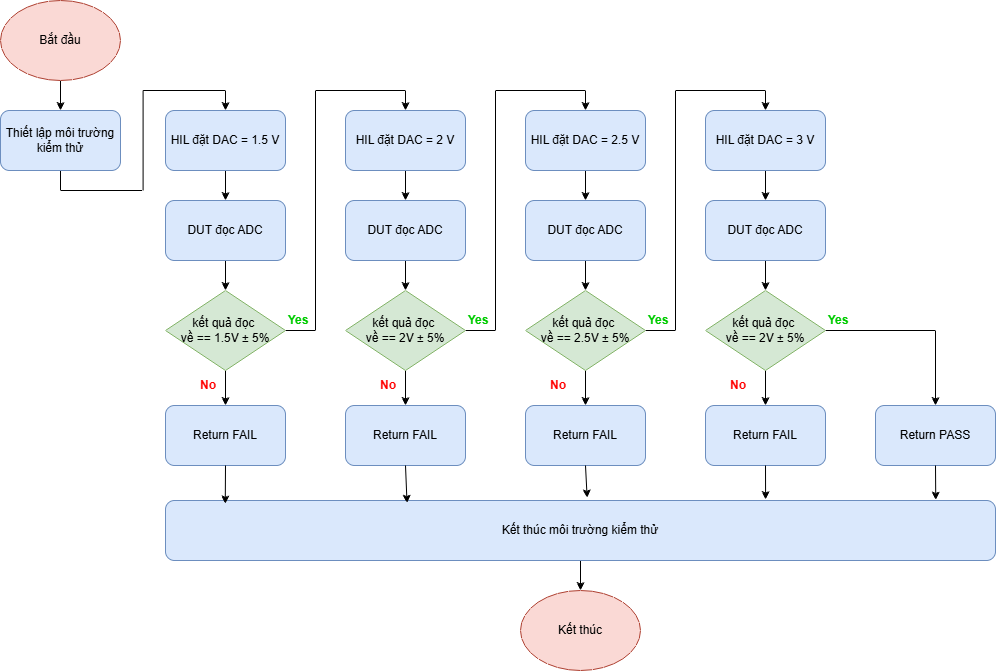
\includegraphics[width=0.7\textwidth]{image/adc_test_flowchart.png}
    \caption{Lưu đồ giải thuật kiểm tra chức năng ADC}
    \label{fig:adc_test_flowchart}
\end{figure}

Trong bài kiểm thử này, hệ thống HIL sử dụng DAC để tạo ra các mức điện áp chuẩn làm tín hiệu đầu vào cho DUT. Việc lựa chọn nhiều mức điện áp khác nhau giúp đánh giá khả năng hoạt động của ADC trên nhiều vùng đo, từ mức điện áp thấp đến mức điện áp gần ngưỡng cực đại của hệ thống.

Firmware trên DUT thực hiện đọc giá trị ADC và chuyển đổi kết quả đo thành giá trị điện áp tương ứng. Giá trị này được gửi về PC thông qua giao tiếp serial để phục vụ quá trình đánh giá.

Hệ thống kiểm thử sẽ so sánh giá trị điện áp DUT đo được với giá trị điện áp do HIL thiết lập trong một khoảng sai số cho phép ( $\pm 5\%$). Việc sử dụng khoảng sai số này giúp phản ánh đúng đặc tính thực tế của bộ ADC, bao gồm sai số chuyển đổi, sai số điện áp tham chiếu và nhiễu tín hiệu trong quá trình đo.

\subsection{Kiểm tra ngoại vi DAC}

Mục đích của bài kiểm thử này là xác minh khả năng tạo tín hiệu analog của DUT thông qua bộ chuyển đổi số sang tương tự (DAC). Bài kiểm thử nhằm đảm bảo firmware cấu hình đúng chức năng DAC, đồng thời tín hiệu analog đầu ra thực tế của DUT đáp ứng đúng dạng sóng và tần số theo yêu cầu thiết kế.

Trong bài kiểm thử này, DUT đóng vai trò chủ động phát sinh tín hiệu analog dưới dạng sóng sine và sóng tam giác với tần số xác định trước. Hệ thống Logic Analyzer được sử dụng để thu thập trực tiếp tín hiệu analog tại chân DAC, sau đó dữ liệu được xử lý và phân tích bằng thuật toán FFT nhằm xác minh đặc tính của dạng sóng đầu ra.

Quy trình kiểm thử tổng quát bao gồm các bước sau:

\begin{itemize}
    \item Bước 1: Thiết lập môi trường kiểm thử bằng cách kết nối HIL, Logic Analyzer, cấp nguồn cho DUT và thiết lập kết nối với DUT.
    \item Bước 2: DUT thực hiện phát tín hiệu sóng sine với tần số xác định trước.
    \item Bước 3: Logic Analyzer thu thập dữ liệu tín hiệu analog tại chân DAC và hệ thống thực hiện phân tích để xác minh tín hiệu có đúng dạng sóng sine và đúng tần số mong đợi hay không.
    \item Bước 4: DUT tiếp tục phát tín hiệu sóng tam giác với tần số xác định trước.
    \item Bước 5: Logic Analyzer tiếp tục thu thập dữ liệu và hệ thống thực hiện phân tích để xác minh tín hiệu có đúng dạng sóng tam giác và đúng tần số mong đợi hay không.
    \item Bước 6: Kết thúc môi trường kiểm thử bằng cách ngắt kết nối DUT, tắt nguồn DUT, ngắt kết nối Logic Analyzer và HIL.
\end{itemize}

Điều kiện đánh giá:

\begin{itemize}
    \item PASS: DUT phát đúng dạng sóng sine và sóng tam giác theo yêu cầu, tần số đo được nằm trong sai số cho phép và các đặc trưng phổ tần phù hợp với dạng sóng mong đợi.
    \item FAIL: Dạng sóng đầu ra không đúng yêu cầu, tần số sai lệch vượt giới hạn cho phép hoặc dữ liệu thu thập không đủ để thực hiện phân tích.
\end{itemize}

Lưu đồ giải thuật tổng quát của bài kiểm thử được trình bày trong Hình \ref{fig:dac_test_flowchart}.

\begin{figure}[H]
    \centering
    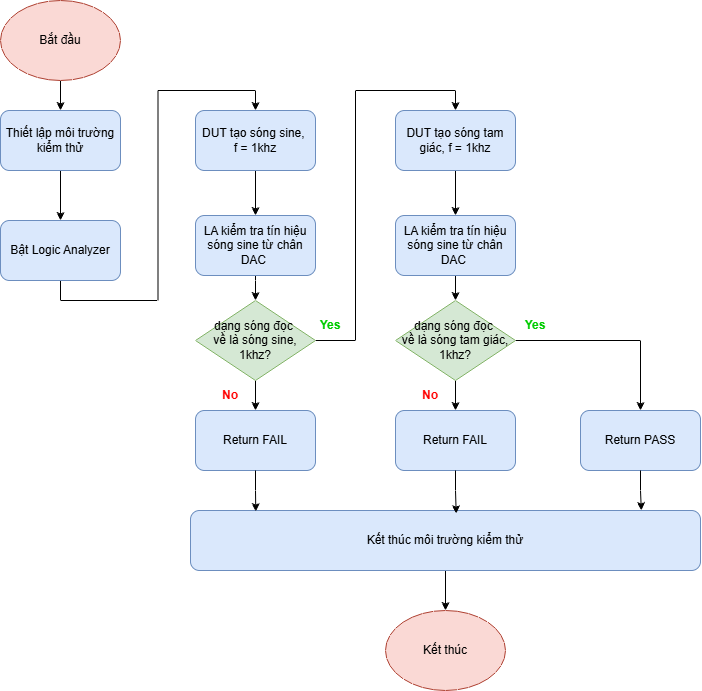
\includegraphics[width=0.8\textwidth]{image/dac_test_flowchart.png}
    \caption{Lưu đồ giải thuật tổng quát kiểm tra chức năng DAC}
    \label{fig:dac_test_flowchart}
\end{figure}

Đối với bài kiểm tra sóng sine, dữ liệu analog thu được từ Logic Analyzer sẽ được chuyển đổi sang miền tần số bằng thuật toán FFT. Hệ thống tiến hành xác định đỉnh năng lượng chính và tính tỷ lệ năng lượng giữa thành phần tín hiệu chính với phần nhiễu còn lại trong phổ tần.

Nếu tỷ lệ năng lượng này (SNR ratio) lớn hơn ngưỡng thực nghiệm đã xác định trước (300), tín hiệu được phân loại là sóng sine. Sau đó, hệ thống tiếp tục kiểm tra tần số đỉnh phổ có nằm trong khoảng sai số cho phép so với tần số mong đợi hay không.

Lưu đồ giải thuật chi tiết của quá trình xác minh sóng sine được trình bày trong Hình \ref{fig:verify_sine_wave_flowchart}.

\begin{figure}[H]
    \centering
    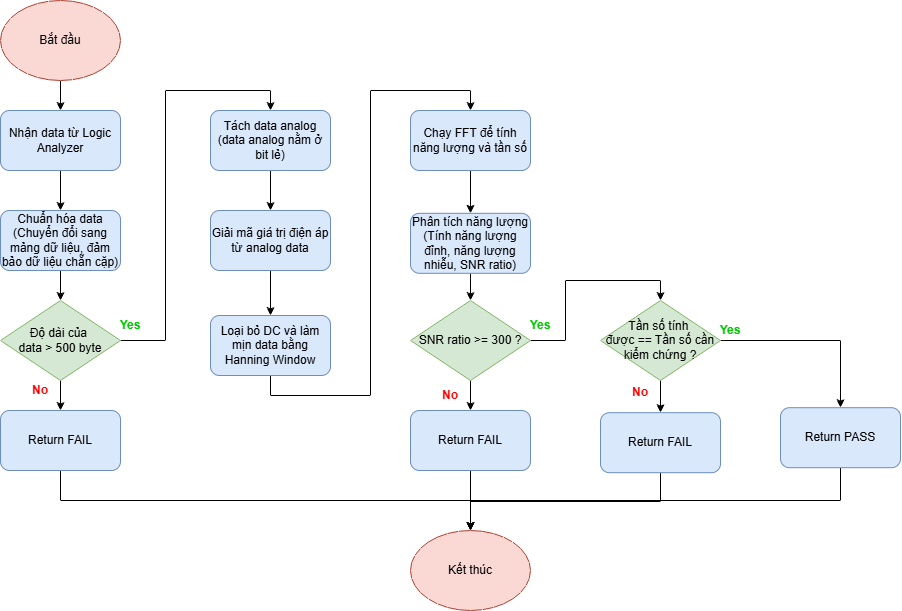
\includegraphics[width=0.8\textwidth]{image/verify_sine_wave_flowchart.png}
    \caption{Lưu đồ giải thuật xác minh sóng sine}
    \label{fig:verify_sine_wave_flowchart}
\end{figure}

Đối với bài kiểm tra sóng tam giác, dữ liệu tín hiệu sau khi xử lý FFT sẽ được phân tích theo đặc trưng phổ hài của sóng triangle. Cụ thể, hệ thống kiểm tra sự suy giảm của các harmonic bậc lẻ và mức năng lượng rất nhỏ của các harmonic bậc chẵn.

Nếu các harmonic chẵn đủ nhỏ và các harmonic lẻ giảm dần đúng đặc tính lý thuyết của sóng tam giác, hệ thống kết luận tín hiệu đầu ra đạt yêu cầu. Sau đó, tần số cơ bản của tín hiệu cũng được so sánh với giá trị mong đợi trong khoảng sai số cho phép.

Lưu đồ giải thuật chi tiết của quá trình xác minh sóng tam giác được trình bày trong Hình \ref{fig:verify_triangle_wave_flowchart}.

\begin{figure}[H]
    \centering
    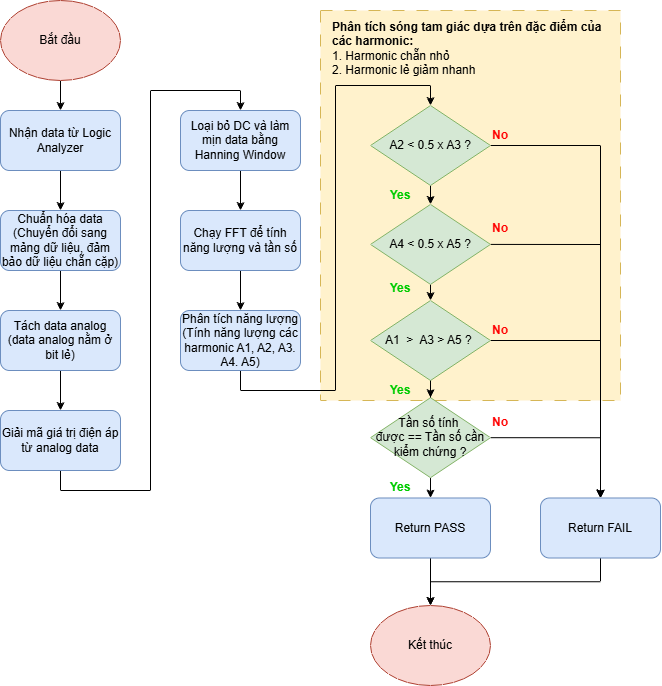
\includegraphics[width=0.8\textwidth]{image/verify_triangle_wave_flowchart.png}
    \caption{Lưu đồ giải thuật xác minh sóng tam giác}
    \label{fig:verify_triangle_wave_flowchart}
\end{figure}

\subsection{Kiểm tra ngoại vi PWM}

Mục đích của bài kiểm thử này là xác minh khả năng tạo tín hiệu điều chế độ rộng xung của DUT, đảm bảo firmware cấu hình đúng tần số và duty cycle của tín hiệu đầu ra theo yêu cầu thiết kế.

Trong bài kiểm thử này, DUT đóng vai trò chủ động phát sinh tín hiệu PWM tại chân đầu ra được chỉ định. Hệ thống Logic Analyzer được sử dụng để thu thập trực tiếp tín hiệu số tại chân PWM, sau đó dữ liệu được xử lý để xác định tần số thực tế và độ rộng xung nhằm so sánh với giá trị mong đợi.

Quy trình kiểm thử tổng quát bao gồm các bước sau:

\begin{itemize}
    \item Bước 1: Thiết lập môi trường kiểm thử bằng cách kết nối HIL, Logic Analyzer, cấp nguồn cho DUT và thiết lập kết nối với DUT.
    \item Bước 2: DUT được cấu hình tần số PWM mong muốn thông qua lệnh thiết lập tần số.
    \item Bước 3: DUT được cấu hình duty cycle tương ứng cho kênh PWM cần kiểm tra.
    \item Bước 4: DUT bắt đầu phát tín hiệu PWM tại chân đầu ra.
    \item Bước 5: Logic Analyzer thu thập dữ liệu tín hiệu số tại chân PWM trong khoảng thời gian xác định.
    \item Bước 6: Hệ thống thực hiện phân tích dữ liệu thu được để xác định tần số thực tế và duty cycle của tín hiệu PWM.
    \item Bước 7: So sánh kết quả đo với giá trị mong đợi trong khoảng sai số cho phép.
    \item Bước 8: DUT dừng phát tín hiệu PWM sau khi hoàn tất kiểm tra.
    \item Bước 9: Đánh giá kết quả kiểm thử và kết thúc môi trường kiểm thử.
\end{itemize}

Điều kiện đánh giá:

\begin{itemize}
    \item PASS: Tín hiệu PWM được tạo đúng với tần số và duty cycle mong đợi, sai số nằm trong giới hạn cho phép ($\pm 5\%$).
    \item FAIL: Tần số hoặc duty cycle đo được sai lệch vượt quá giới hạn cho phép, tín hiệu không được phát ra hoặc dữ liệu thu thập không đủ để phân tích.
\end{itemize}

Lưu đồ giải thuật tổng quát của bài kiểm thử được trình bày trong Hình \ref{fig:pwm_test_flowchart}.

\begin{figure}[H]
    \centering
    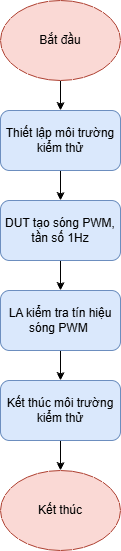
\includegraphics[height=0.4\textheight]{image/pwm_test_flowchart.png}
    \caption{Lưu đồ giải thuật tổng quát kiểm tra chức năng PWM}
    \label{fig:pwm_test_flowchart}
\end{figure}

Trong bài kiểm thử này, Logic Analyzer thực hiện thu thập dữ liệu số tại chân PWM và tách riêng kênh digital tương ứng để phân tích. Thuật toán kiểm tra được xây dựng dựa trên phương pháp phát hiện cạnh lên nhằm xác định chu kỳ tín hiệu.

Từ vị trí các cạnh lên liên tiếp, hệ thống tính toán thời gian của nhiều chu kỳ PWM để xác định tần số thực tế của tín hiệu. Đồng thời, tỷ lệ thời gian mức logic cao trên toàn bộ chu kỳ được sử dụng để tính duty cycle thực tế.

Sau khi thu được hai thông số này, hệ thống tiến hành so sánh với giá trị mong đợi đã cấu hình trước đó. Sai số cho phép được lựa chọn là $\pm 5\%$ nhằm phản ánh đúng đặc tính thực tế của hệ thống nhúng và giới hạn sai số đo của thiết bị.

Lưu đồ giải thuật chi tiết của quá trình xác minh tín hiệu PWM được trình bày trong Hình \ref{fig:verify_pwm_flowchart}.

\begin{figure}[H]
    \centering
    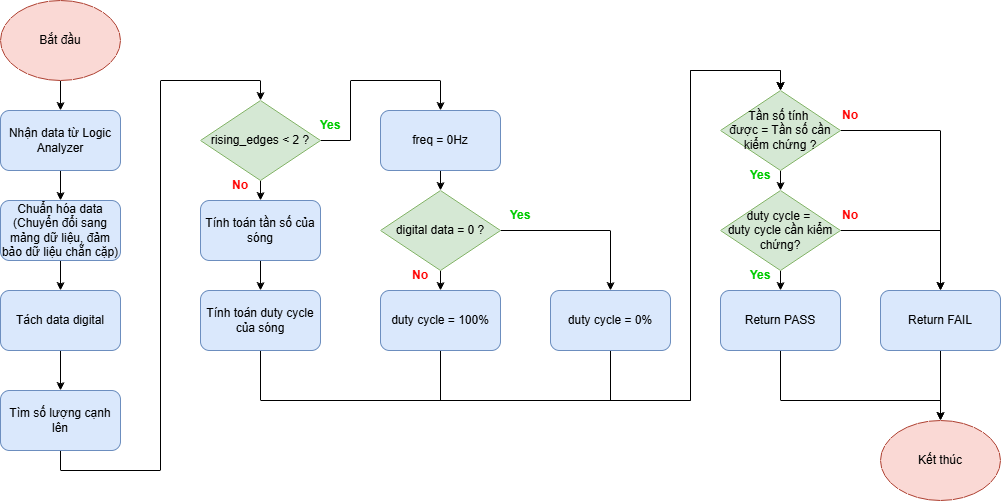
\includegraphics[width=0.85\textwidth]{image/verify_pwm_flowchart.png}
    \caption{Lưu đồ giải thuật xác minh tín hiệu PWM}
    \label{fig:verify_pwm_flowchart}
\end{figure}

\subsection{Kiểm tra ngoại vi UART}

Mục đích của bài kiểm thử này là xác minh khả năng truyền và nhận dữ liệu nối tiếp UART giữa DUT và hệ thống HIL, đảm bảo firmware cấu hình đúng giao tiếp UART và dữ liệu truyền nhận giữa hai thiết bị được thực hiện chính xác theo cả hai chiều.

Trong bài kiểm thử này, cả DUT và HIL đều được cấu hình giao tiếp UART với cùng thông số truyền thông như baudrate, số bit dữ liệu, bit chẵn lẻ và bit stop. Quá trình kiểm thử được thực hiện theo hai hướng truyền dữ liệu: từ DUT sang HIL và từ HIL sang DUT nhằm xác minh đầy đủ khả năng truyền nhận hai chiều của hệ thống.

Quy trình kiểm thử tổng quát bao gồm các bước sau:

\begin{itemize}
    \item Bước 1: Thiết lập môi trường kiểm thử bằng cách kết nối HIL, cấp nguồn cho DUT và thiết lập kết nối với DUT.
    \item Bước 2: Khởi tạo giao tiếp UART trên cả HIL và DUT với cùng cấu hình truyền thông.
    \item Bước 3: Thực hiện kiểm thử truyền dữ liệu từ DUT sang HIL bằng cách DUT gửi chuỗi dữ liệu kiểm thử và HIL đọc dữ liệu nhận được để so sánh với giá trị mong đợi.
    \item Bước 4: Thực hiện kiểm thử truyền dữ liệu từ HIL sang DUT bằng cách HIL gửi chuỗi dữ liệu kiểm thử và DUT đọc dữ liệu nhận được để so sánh với giá trị mong đợi.
    \item Bước 5: Đánh giá kết quả kiểm thử dựa trên toàn bộ phản hồi thu được từ cả hai chiều truyền dữ liệu.
    \item Bước 6: Kết thúc môi trường kiểm thử bằng cách ngắt kết nối DUT, tắt nguồn DUT và ngắt kết nối HIL.
\end{itemize}

Điều kiện đánh giá:

\begin{itemize}
    \item PASS: Dữ liệu truyền nhận ở cả hai chiều DUT → HIL và HIL → DUT đều chính xác, chuỗi nhận được khớp hoàn toàn với chuỗi dữ liệu mong đợi.
    \item FAIL: Có ít nhất một chiều truyền dữ liệu bị lỗi, dữ liệu nhận được không đầy đủ, sai nội dung hoặc không nhận được phản hồi.
\end{itemize}

Lưu đồ giải thuật tổng quát của bài kiểm thử được trình bày trong Hình \ref{fig:uart_test_flowchart}.

\begin{figure}[H]
    \centering
    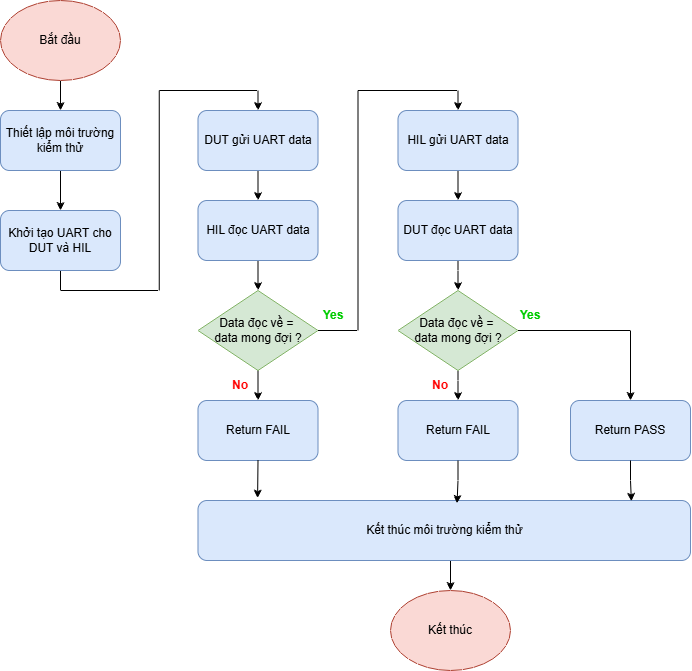
\includegraphics[width=0.8\textwidth]{image/uart_test_flowchart.png}
    \caption{Lưu đồ giải thuật tổng quát kiểm tra chức năng UART}
    \label{fig:uart_test_flowchart}
\end{figure}

\subsection{Kiểm tra ngoại vi CAN}

(Nên chia nhỏ bài test ra để test từng chức năng riêng: CAN receive, CAN transmit thay vì gộp chung như hiện tại. Cần Update thêm function cho CAN test case: Long Payload Transmission, Continuous Transmission)

Mục đích của bài kiểm thử này là xác minh khả năng truyền và nhận dữ liệu của DUT thông qua giao tiếp CAN, đảm bảo firmware cấu hình đúng ngoại vi CAN và dữ liệu trao đổi giữa DUT với hệ thống HIL được thực hiện chính xác, ổn định và không xảy ra lỗi truyền thông.

Trong bài kiểm thử này, hệ thống HIL đóng vai trò mô phỏng node giao tiếp CAN với DUT. HIL thực hiện gửi các khung dữ liệu CAN đến DUT, đồng thời đọc dữ liệu phản hồi từ DUT để kiểm tra tính chính xác của quá trình truyền nhận. Việc kiểm thử được thực hiện với cả dữ liệu dạng buffer tuần tự và dữ liệu dạng chuỗi ký tự nhằm đánh giá nhiều tình huống truyền thông khác nhau.

Quy trình kiểm thử tổng quát bao gồm các bước sau:

\begin{itemize}
    \item Bước 1: Thiết lập môi trường kiểm thử bằng cách kết nối HIL và cấp nguồn cho DUT.
    \item Bước 2: Hệ thống HIL gửi một khung dữ liệu CAN dạng buffer tuần tự đến DUT để kiểm tra khả năng truyền nhận dữ liệu nhị phân.
    \item Bước 3: HIL đọc dữ liệu phản hồi từ DUT và kiểm tra tính đúng đắn của dữ liệu bằng quy tắc tăng tuần tự giữa các byte.
    \item Bước 4: Hệ thống HIL gửi một chuỗi dữ liệu dạng ký tự đến DUT thông qua giao tiếp CAN để kiểm tra khả năng xử lý dữ liệu dạng text.
    \item Bước 5: HIL tiếp tục đọc dữ liệu phản hồi từ DUT và so sánh với chuỗi dữ liệu mong đợi.
    \item Bước 6: Đánh giá kết quả kiểm thử dựa trên toàn bộ phản hồi thu được.
    \item Bước 7: Kết thúc môi trường kiểm thử bằng cách ngắt kết nối HIL.
\end{itemize}

Điều kiện đánh giá:

\begin{itemize}
    \item PASS: Dữ liệu CAN nhận được từ DUT ở cả hai bài kiểm thử buffer và string đều chính xác, đúng thứ tự và khớp với giá trị mong đợi.
    \item FAIL: Có ít nhất một khung dữ liệu bị mất, sai nội dung, sai thứ tự hoặc DUT không phản hồi dữ liệu CAN đúng yêu cầu.
\end{itemize}

Lưu đồ giải thuật tổng quát của bài kiểm thử được trình bày trong Hình \ref{fig:can_test_flowchart}.

\begin{figure}[H]
    \centering
    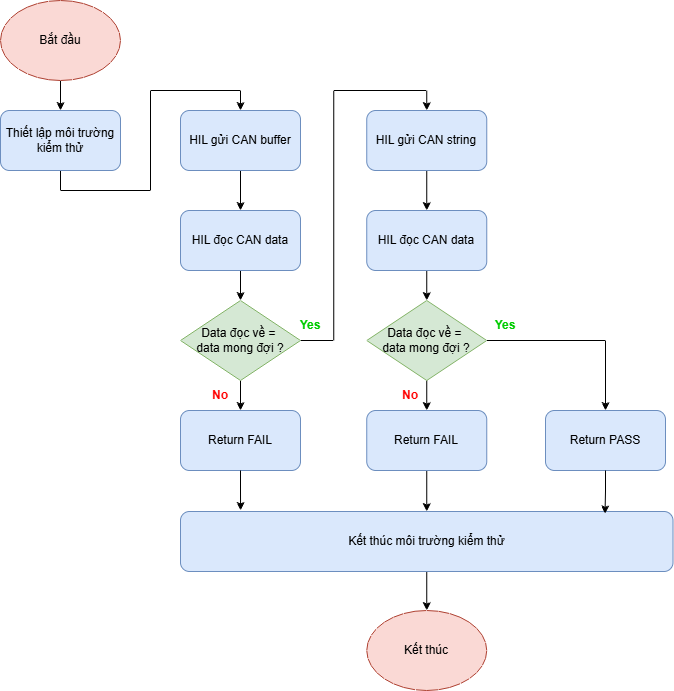
\includegraphics[width=0.8\textwidth]{image/can_test_flowchart.png}
    \caption{Lưu đồ giải thuật tổng quát kiểm tra chức năng CAN}
    \label{fig:can_test_flowchart}
\end{figure}

\subsection{Kiểm tra giao tiếp I2C với EEPROM}

Mục đích của bài kiểm thử này là xác minh khả năng giao tiếp giữa DUT và bộ nhớ ngoài EEPROM thông qua giao thức I2C, đảm bảo firmware cấu hình đúng ngoại vi I2C, thực hiện ghi và đọc dữ liệu chính xác, đồng thời đáp ứng yêu cầu về thời gian ghi dữ liệu.

Trong bài kiểm thử này, hệ thống HIL đóng vai trò mô phỏng thiết bị EEPROM với các tham số cấu hình như địa chỉ I2C, dung lượng bộ nhớ và kích thước trang. DUT thực hiện các thao tác đọc và ghi dữ liệu lên EEPROM thông qua giao tiếp I2C, sau đó phản hồi kết quả về PC để phục vụ quá trình đánh giá.

Quy trình kiểm thử tổng quát bao gồm các bước sau:

\begin{itemize}
    \item Bước 1: Thiết lập môi trường kiểm thử bằng cách kết nối HIL, cấp nguồn cho DUT và thiết lập kết nối với DUT.
    \item Bước 2: Hệ thống HIL khởi tạo mô hình EEPROM với các tham số cấu hình (địa chỉ, dung lượng, kích thước trang) và kích hoạt thiết bị trên bus I2C.
    \item Bước 3: DUT thực hiện khởi tạo giao tiếp với EEPROM thông qua I2C.
    \item Bước 4: DUT thực hiện ghi dữ liệu xuống EEPROM và đo thời gian ghi tương ứng với một khối dữ liệu xác định.
    \item Bước 5: Hệ thống kiểm thử đánh giá thời gian ghi có nằm trong giới hạn cho phép hay không.
    \item Bước 6: DUT thực hiện ghi và đọc lại dữ liệu từ EEPROM, sau đó gửi dữ liệu đọc được về PC.
    \item Bước 7: Hệ thống kiểm thử so sánh dữ liệu đọc được với dữ liệu mong đợi để xác minh tính toàn vẹn dữ liệu.
    \item Bước 8: Đánh giá kết quả kiểm thử dựa trên toàn bộ phản hồi thu được.
    \item Bước 9: Kết thúc môi trường kiểm thử bằng cách giải phóng tài nguyên EEPROM trên HIL.
\end{itemize}

\textbf{Điều kiện đánh giá:}

\begin{itemize}
    \item PASS: 
    \begin{itemize}
        \item HIL khởi tạo EEPROM thành công.
        \item DUT truy cập được EEPROM tại địa chỉ đã cấu hình.
        \item Thời gian ghi dữ liệu của DUT nhỏ hơn ngưỡng cho phép.
        \item Dữ liệu ghi vào EEPROM được đọc lại chính xác, đúng thứ tự và không bị sai lệch.
    \end{itemize}

    \item FAIL: Bài kiểm thử sẽ trả về FAIL nếu xảy ra bất kỳ lỗi nào sau đây:
    \begin{itemize}
        \item HIL không khởi tạo được EEPROM (sai địa chỉ, sai giá trị cấu hình).
        \item EEPROM không được phát hiện trên bus I2C.
        \item DUT không giao tiếp được với EEPROM (không phát hiện được thiết bị hoặc không đọc/ghi được).
        \item Thời gian ghi dữ liệu vượt quá ngưỡng cho phép.
        \item Dữ liệu đọc lại không khớp với dữ liệu đã ghi (mất dữ liệu, sai thứ tự).
    \end{itemize}
\end{itemize}

Lưu đồ giải thuật tổng quát của bài kiểm thử được trình bày trong Hình \ref{fig:eeprom_test_flowchart}.

\begin{figure}[H]
    \centering
    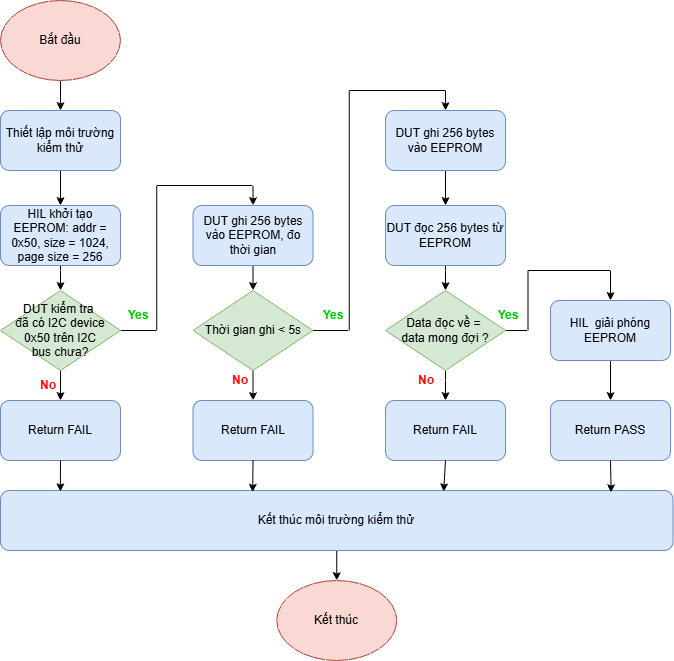
\includegraphics[width=0.8\textwidth]{image/eeprom_test_flowchart.png}
    \caption{Lưu đồ giải thuật kiểm tra chức năng EEPROM thông qua giao tiếp I2C}
    \label{fig:eeprom_test_flowchart}
\end{figure}.

\subsection{Kiểm tra giao tiếp I2C với RTC}

Mục đích của bài kiểm thử này là xác minh khả năng giao tiếp giữa DUT với bộ thời gian thực RTC.

Trong bài kiểm thử này, hệ thống HIL đóng vai trò mô phỏng và kích hoạt thiết bị RTC trên bus I2C. DUT thực hiện các thao tác thiết lập và đọc dữ liệu từ RTC, sau đó gửi kết quả về PC để phục vụ quá trình kiểm tra và đánh giá.

Quy trình kiểm thử tổng quát bao gồm các bước sau:

\begin{itemize}
    \item Bước 1: Thiết lập môi trường kiểm thử bằng cách kết nối HIL, cấp nguồn cho DUT và thiết lập kết nối với DUT.
    \item Bước 2: HIL khởi tạo thiết bị RTC tại địa chỉ I2C tương ứng và kích hoạt thiết bị trên bus.
    \item Bước 3: DUT khởi tạo RTC và thiết lập thời gian (giờ, phút, giây) và ngày tháng (thứ, ngày, tháng, năm).
    \item Bước 4: DUT đọc lại giá trị thời gian và ngày tháng từ RTC, hệ thống so sánh với giá trị mong đợi trong khoảng sai số cho phép.
    \item Bước 5: Kiểm tra khả năng tự động tăng thời gian của RTC bằng cách thiết lập thời điểm gần thời điểm chuyển ngày, sau đó chờ một khoảng thời gian xác định.
    \item Bước 6: DUT đọc lại thời gian và ngày tháng sau khi chờ, hệ thống kiểm tra việc chuyển sang ngày mới và giá trị thời gian có đúng hay không.
    \item Bước 7: Đánh giá kết quả kiểm thử dựa trên toàn bộ dữ liệu thu được.
    \item Bước 8: Kết thúc môi trường kiểm thử bằng cách tắt nguồn DUT và ngắt kết nối HIL.
\end{itemize}

\textbf{Điều kiện đánh giá:}

\begin{itemize}
    \item PASS:
    \begin{itemize}
        \item HIL khởi tạo và kích hoạt thành công thiết bị RTC trên bus I2C.
        \item DUT thiết lập và đọc lại chính xác giá trị thời gian và ngày tháng từ RTC.
        \item Sai số thời gian nằm trong khoảng cho phép (do độ trễ xử lý và thời gian giao tiếp).
        \item RTC tự động tăng thời gian chính xác và chuyển ngày đúng khi vượt qua mốc 00:00:00.
    \end{itemize}

    \item FAIL: Bài kiểm thử sẽ trả về FAIL nếu xảy ra bất kỳ lỗi nào sau đây:
    \begin{itemize}
        \item HIL không khởi tạo hoặc không kích hoạt được thiết bị RTC.
        \item DUT không giao tiếp được với RTC (không đọc/ghi được dữ liệu).
        \item Giá trị thời gian hoặc ngày tháng đọc được không khớp với giá trị đã thiết lập.
        \item Sai số thời gian vượt quá ngưỡng cho phép.
        \item RTC không tăng thời gian đúng hoặc không chuyển ngày khi vượt qua mốc thời gian.
    \end{itemize}
\end{itemize}

Lưu đồ giải thuật tổng quát của bài kiểm thử được trình bày trong Hình \ref{fig:rtc_test_flowchart}.

\begin{figure}[H]
    \centering
    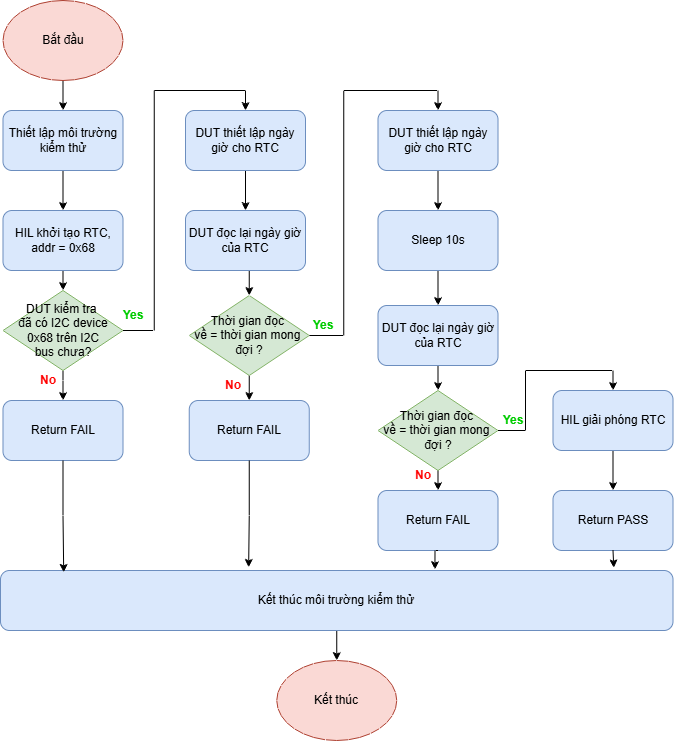
\includegraphics[width=0.8\textwidth]{image/rtc_test_flowchart.png}
    \caption{Lưu đồ giải thuật tổng quát kiểm tra chức năng RTC}
    \label{fig:rtc_test_flowchart}
\end{figure}

\subsection{Kiểm tra giao tiếp SPI với FLASH}

Mục đích của bài kiểm thử này là xác minh khả năng giao tiếp và thao tác với bộ nhớ SPI Flash của DUT, bao gồm việc đọc ID thiết bị, đọc dữ liệu, ghi dữ liệu và xóa dữ liệu. Bài kiểm thử nhằm đảm bảo firmware cấu hình đúng giao tiếp SPI và các thao tác trên bộ nhớ Flash được thực hiện chính xác, ổn định.

Trong bài kiểm thử này, hệ thống HIL đóng vai trò chuẩn bị dữ liệu mẫu trong SPI Flash để DUT đọc và kiểm tra. DUT thực hiện các thao tác đọc, ghi và xóa dữ liệu trên SPI Flash, sau đó gửi kết quả về PC để tiến hành đánh giá.

Quy trình kiểm thử tổng quát bao gồm các bước sau:

\begin{itemize}
    \item Bước 1: Thiết lập môi trường kiểm thử bằng cách kết nối HIL, cấp nguồn cho DUT và thiết lập kết nối với DUT.
    \item Bước 2: DUT thực hiện đọc ID của SPI Flash để xác minh kết nối phần cứng và nhận diện thiết bị.
    \item Bước 3: HIL chuẩn bị dữ liệu mẫu với độ dài xác định (512 bytes) trong bộ nhớ SPI Flash.
    \item Bước 4: DUT đọc dữ liệu từ SPI Flash và hệ thống kiểm tra tính đúng đắn của dữ liệu theo quy luật tăng tuần tự.
    \item Bước 5: DUT thực hiện xóa dữ liệu trong SPI Flash.
    \item Bước 6: DUT đọc lại dữ liệu sau khi xóa và hệ thống kiểm tra trạng thái dữ liệu đã được xóa hoàn toàn.
    \item Bước 7: DUT ghi dữ liệu mới vào SPI Flash với độ dài lớn hơn (1024 bytes).
    \item Bước 8: DUT đọc lại dữ liệu vừa ghi và hệ thống kiểm tra tính chính xác của dữ liệu.
    \item Bước 9: Đánh giá kết quả kiểm thử dựa trên toàn bộ dữ liệu thu được.
    \item Bước 10: Kết thúc môi trường kiểm thử bằng cách ngắt kết nối HIL và DUT.
\end{itemize}

\textbf{Điều kiện đánh giá:}

\begin{itemize}
    \item PASS:
    \begin{itemize}
        \item DUT đọc được đúng ID của SPI Flash, xác nhận thiết bị hoạt động bình thường.
        \item Dữ liệu đọc từ SPI Flash (do HIL chuẩn bị) chính xác và đúng thứ tự.
        \item Sau khi thực hiện lệnh xóa, toàn bộ dữ liệu trong vùng nhớ được đưa về trạng thái đã xóa (thường là 0xFF).
        \item Dữ liệu ghi mới vào SPI Flash được đọc lại chính xác, không bị sai lệch.
    \end{itemize}

    \item FAIL: Bài kiểm thử sẽ trả về FAIL nếu xảy ra bất kỳ lỗi nào sau đây:
    \begin{itemize}
        \item DUT không đọc được ID hoặc ID không đúng với thiết bị SPI Flash.
        \item Dữ liệu đọc từ SPI Flash bị sai, thiếu hoặc không đúng thứ tự.
        \item Quá trình xóa không thành công (dữ liệu sau khi xóa không đồng nhất).
        \item Dữ liệu ghi vào SPI Flash bị sai lệch khi đọc lại.
        \item DUT không phản hồi hoặc xảy ra lỗi trong quá trình giao tiếp SPI.
    \end{itemize}
\end{itemize}

Lưu đồ giải thuật tổng quát của bài kiểm thử được trình bày trong Hình \ref{fig:spi_flash_test_flowchart}.

\begin{figure}[H]
    \centering
    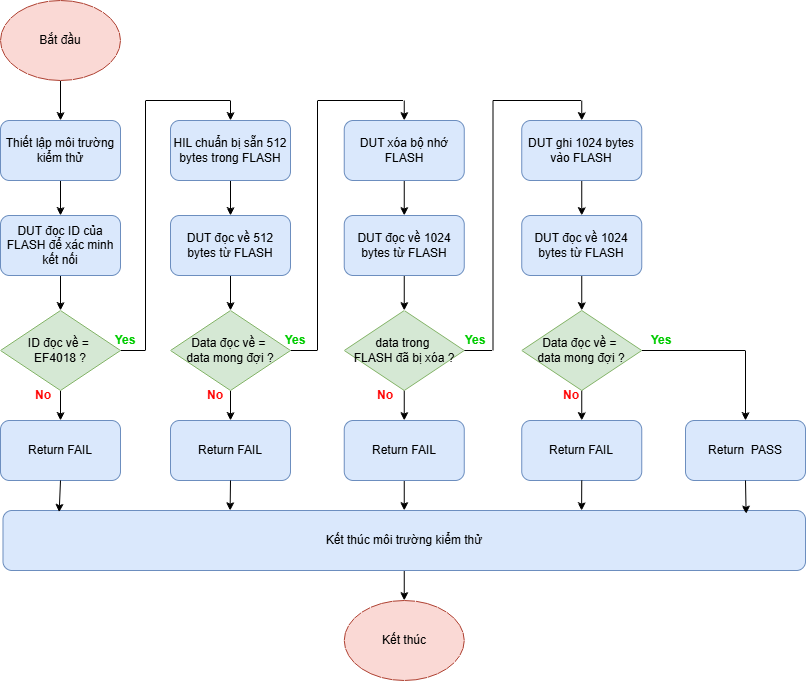
\includegraphics[width=0.8\textwidth]{image/spi_flash_test_flowchart.png}
    \caption{Lưu đồ giải thuật tổng quát kiểm tra chức năng SPI Flash}
    \label{fig:spi_flash_test_flowchart}
\end{figure}
.

\newpage
\chapter{KẾT QUẢ THỰC HIỆN}

Chương này trình bày các kết quả đạt được sau quá trình thiết kế, xây dựng và triển khai hệ thống Hardware-in-the-Loop cho kiểm thử phần mềm nhúng. Các kết quả được phân tích theo ba thành phần chính của hệ thống bao gồm: phần mềm HIL, phần mềm giao diện trên máy tính và phần mềm kiểm thử tự động. Qua đó đánh giá mức độ đáp ứng yêu cầu thiết kế cũng như khả năng ứng dụng thực tế của hệ thống.

\section{Kết quả thực hiện phần mềm HIL}

\subsection{Kết quả mô phỏng ngoại vi}
\subsubsection{Kêt quả mô phỏng GPIO}
(thêm bảng số lượng chân GPIO support, các chế độ hoạt động, mức điện áp logic)

\subsubsection{Kết quả mô phỏng ADC}
(thêm bảng số lượng chân ADC support, dải điện áp đo được, độ phân giải ADC)

\subsubsection{Kết quả mô phỏng DAC}
(thêm bảng số lượng chân DAC support, dải điện áp đầu ra, độ phân giải DAC)
(kết quả tạo sóng sine wave, triangle wave)

\subsubsection{Kết quả mô phỏng PWM}
(thêm bảng số lượng chân PWM support, dải tần số, kết quả tạo tín hiệu PWM với tần số và duty cycle khác nhau)

\subsubsection{Kết quả mô phỏng UART}
(thêm bảng số lượng cổng UART support, tốc độ baud rate hỗ trợ, kết quả gửi nhận dữ liệu qua UART)
\subsubsection{Kết quả mô phỏng CAN}
(thêm bảng số lượng cổng CAN support, tốc độ baud rate hỗ trợ, kết quả gửi nhận dữ liệu qua CAN)

\subsection{Kết quả mô phỏng thiết bị}
\subsubsection{Kết quả mô phỏng I2C EEPROM}
(thêm bảng kết quả kiểm thử đọc ghi dữ liệu vào I2C EEPROM mô phỏng, bao gồm địa chỉ, dữ liệu đã ghi, dữ liệu đã đọc và kết quả so sánh)

\subsubsection{Kết quả mô phỏng I2C RTC}
(thêm bảng kết quả kiểm thử thiết lập và đọc thời gian từ RTC mô phỏng, bao gồm thời gian đã thiết lập, thời gian đã đọc và kết quả so sánh)
\subsubsection{Kết quả mô phỏng SPI Flash}
(thêm bảng kết quả kiểm thử đọc ghi dữ liệu vào SPI Flash mô phỏng, bao gồm địa chỉ, dữ liệu đã ghi, dữ liệu đã đọc và kết quả so sánh)

\subsection{Đánh giá kết quả}
(thêm bảng các pin support)

\section{Kết quả thực hiện phần mềm Logic Analyzer trên HIL}

\section{Kết quả thực hiện phần mềm trên máy tính}
Giao diện chính của phần mềm được tổ chức dưới dạng các tab riêng biệt nhằm tăng tính trực quan và thuận tiện trong quá trình sử dụng, bao gồm:
\begin{itemize}
    \item \textbf{Serial Tab}: Cấu hình các  thông số cho Serial port (cổng COM, baudrate).
    \item \textbf{Terminal Tab}: Hỗ trợ giao diện dòng lệnh cho người dùng nhập lệnh thủ công.
    \item \textbf{Memory EMU Tab}: Hỗ trợ người dùng thao tác với thiết bị bộ nhớ mô phỏng trên HIL như SPI Flash và I2C EEPROM.
    \item \textbf{Logic Analyzer Tab}: Hiển thị tín hiệu digital, analog giúp người dùng có thể quan sát và phân tích các tín hiệu như tần số, dạng sóng,...
    \item \textbf{Peripherals Tab}: Hỗ trợ người dùng thao tác với các thiết bị ngoại vi khác như GPIO, ADC, DAC,... để kiểm thử DUT.
\end{itemize}
\begin{figure}[H]
    \centering
    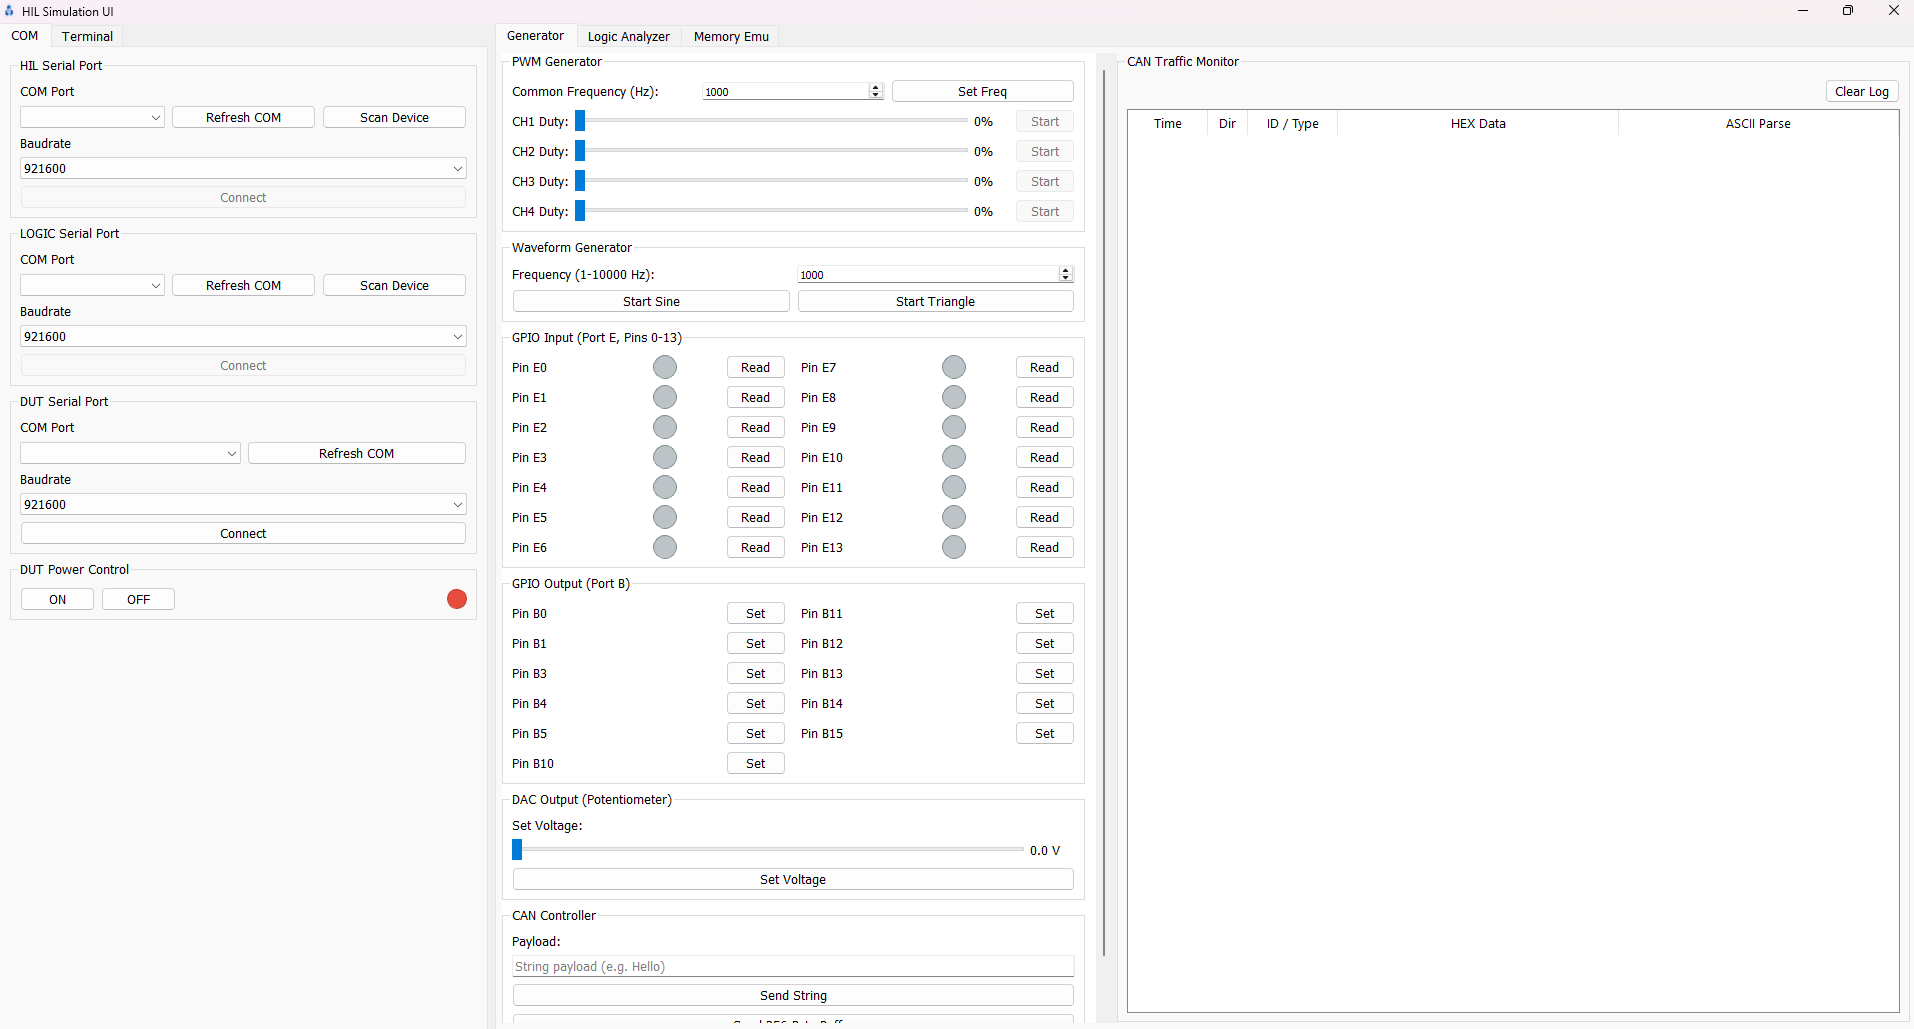
\includegraphics[width=1\textwidth]{image/PC_GUI.png}
    \caption{Giao diện chính của phần mềm trên máy tính}
    \label{fig:PC_GUI}
\end{figure}

\subsection{Kết quả điều khiển nguồn cho DUT}
Người dùng sẽ được cung cấp các nút nhấn trên giao diện để điều khiển nguồn cho DUT.
\begin{figure}[H]
    \centering
    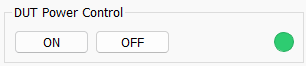
\includegraphics[width=0.7\textwidth]{image/power_on.png}
    \caption{Bật nguồn DUT}
    \label{fig:power_on}
\end{figure}

\begin{figure}[H]
    \centering
    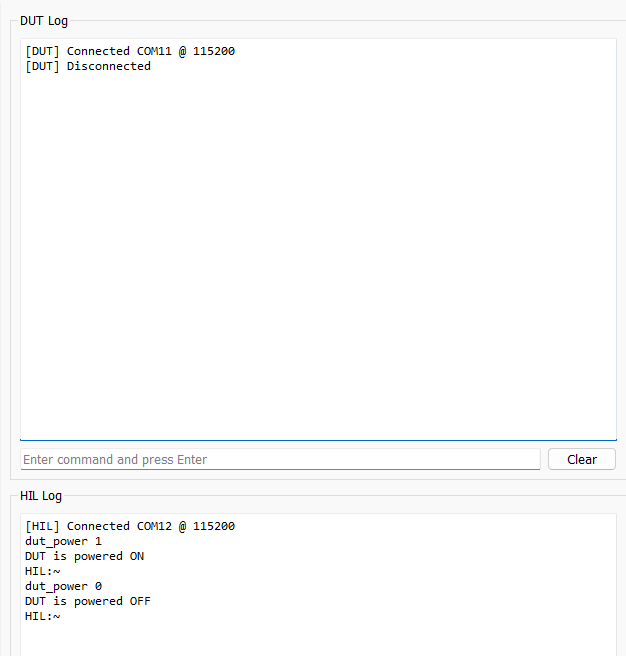
\includegraphics[width=0.7\textwidth]{image/power_off.png}
    \caption{Tắt nguồn DUT}
    \label{fig:power_off}
\end{figure}

\begin{figure}[H]
    \centering
    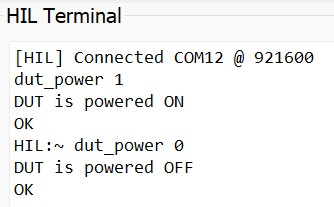
\includegraphics[width=0.5\textwidth]{image/power_app.jpg}
    \caption{Trạng thái nguồn của DUT trong giao diện dòng lệnh}
    \label{fig:power_app}
\end{figure}
\textbf{Nhận xét:} Dựa trên các kết quả từ giao diện UI và giao diện dòng lệnh, có thể thấy nguồn của DUT đã được bật/tắt và trạng thái nguồn được cập nhật qua led trên phần mềm.

\subsection{Kết quả mô phỏng SPI Flash}
Người dùng có thể dùng giao diện dòng lệnh để gửi các command thủ công cho DUT để thực hiện các thao tác đọc ghi dữ liệu vào SPI Flash mô phỏng. Ngoài ra, phần mềm trên máy tính được thiết kế để thực hiện 1 bài kiểm thử tự động để kiểm tra chức năng đọc/ghi dữ liệu của DUT với thiết bị SPI Flash mô phỏng trên hệ thống HIL. Các bước thực hiện bao gồm:
\begin{itemize}
    \item \textbf{Bước 1:} PC gửi lệnh đến \textbf{DUT} đọc ID của thiết bị SPI Flash (HIL đang mô phỏng W25Q128 với ID: 0xEF4018).\\
    \begin{figure}[H]
        \centering
        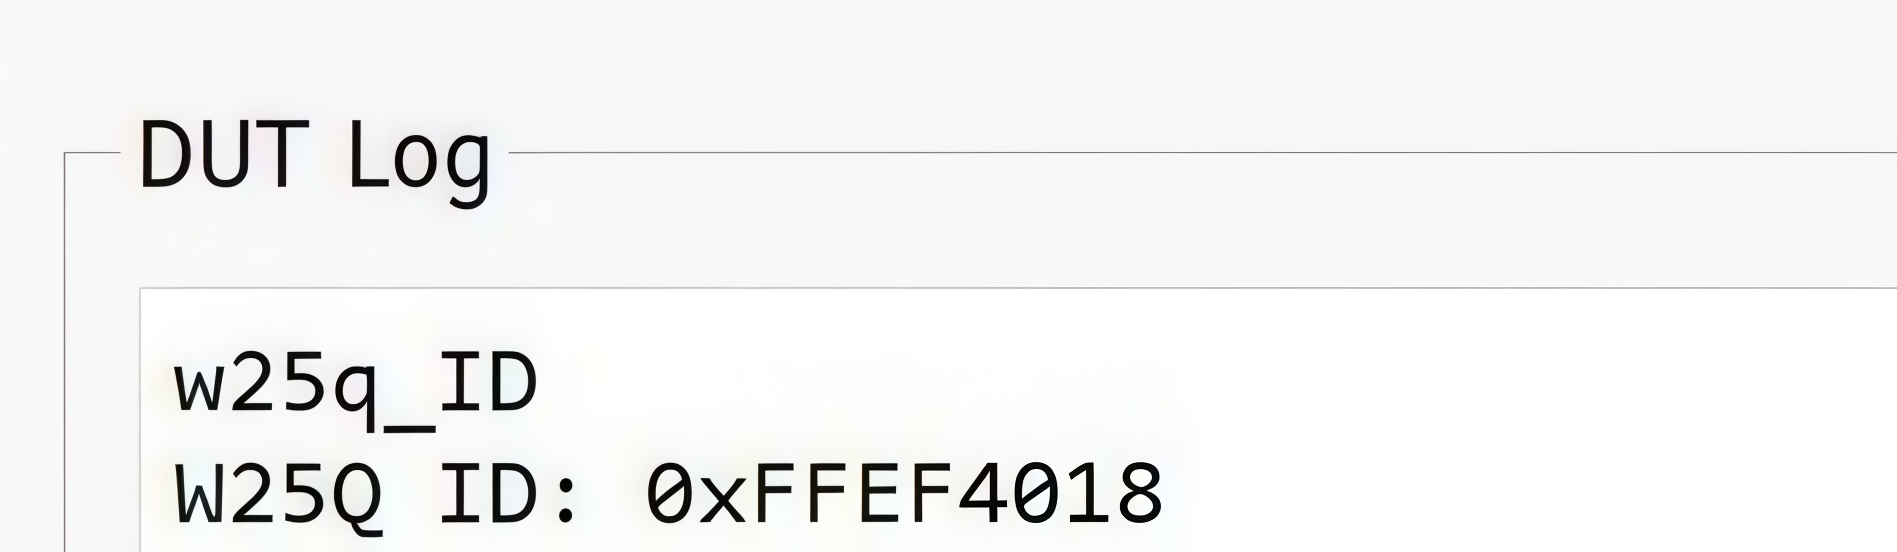
\includegraphics[width=0.8\textwidth]{image/spi_read_id.jpg}
        \caption{DUT đọc ID của thiết bị SPI Flash mô phỏng trên HIL}
        \label{fig:spi_read_id}
    \end{figure}

    \item \textbf{Bước 2:} PC gửi lệnh đến \textbf{HIL} để khởi tạo bộ nhớ từ địa chỉ 0 - 255 với giá trị tăng dần từ 0x00 đến 0xFF.\\
    \begin{figure}[H]
        \centering
        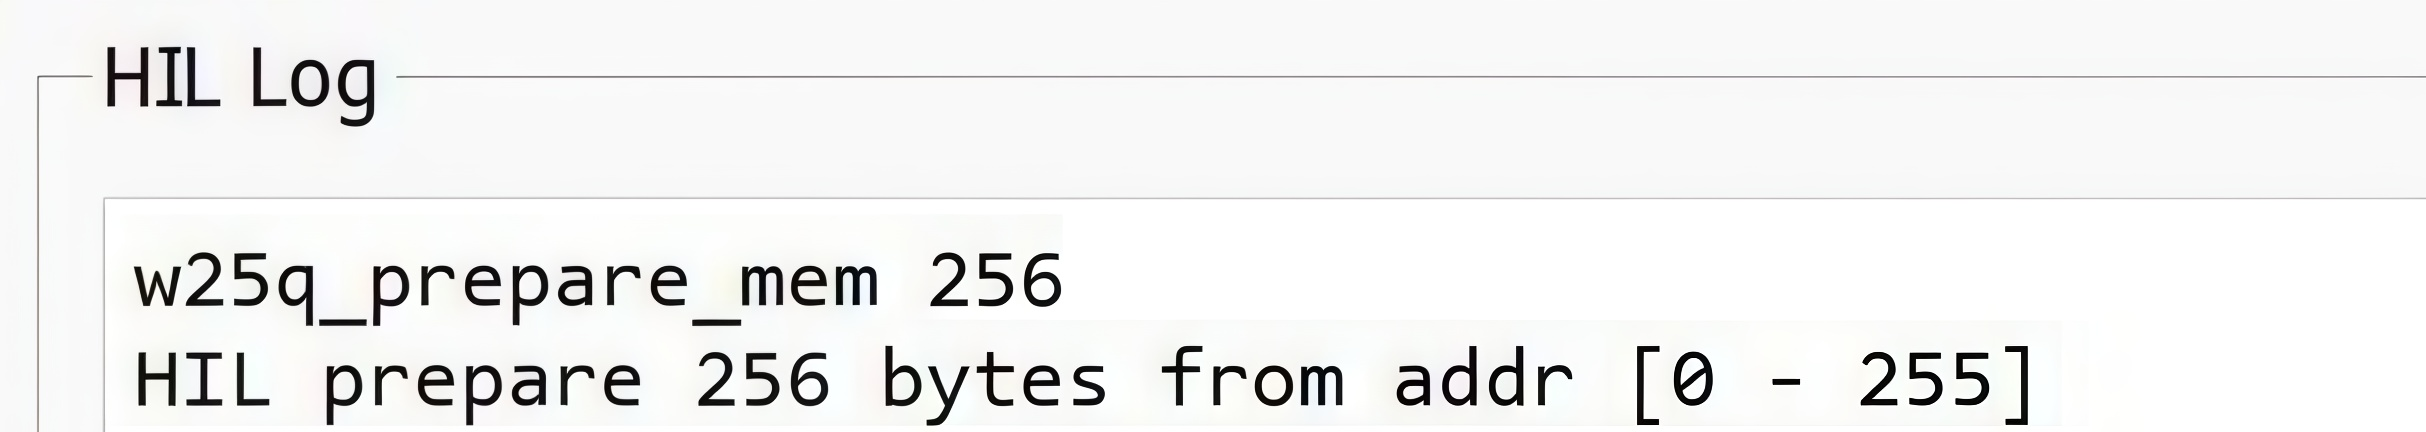
\includegraphics[width=0.8\textwidth]{image/spi_hil_prepare_mem.jpg}
        \caption{HIL khởi tạo bộ nhớ SPI Flash mô phỏng}
        \label{fig:spi_hil_prepare_mem}
    \end{figure}

    \item \textbf{Bước 3:} PC gửi lệnh đến \textbf{DUT}, yêu cầu DUT đọc vào vùng nhớ từ 0 - 255 mà thiết bị SPI Flash mô phỏng trên HIL. Dữ liệu đọc được sẽ được gửi lại PC để so sánh với dữ liệu gốc.\\
    \begin{figure}[H]
        \centering
        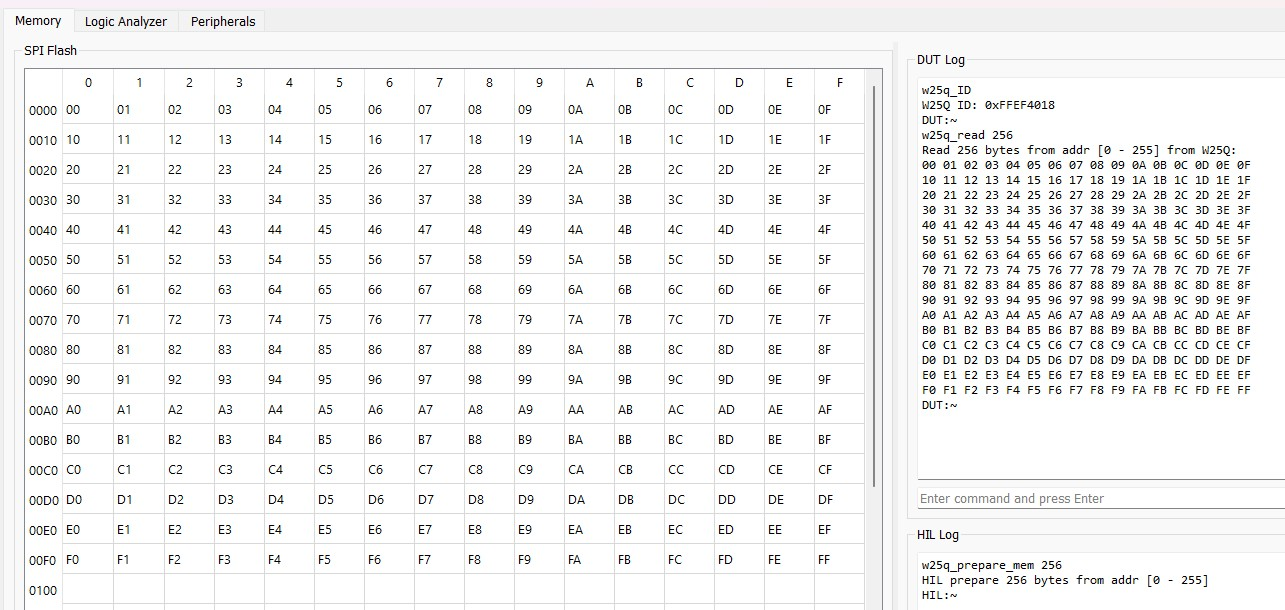
\includegraphics[width=1\textwidth]{image/spi_read_256.jpg}
        \caption{DUT đọc dữ liệu từ SPI Flash mô phỏng}
        \label{fig:spi_read_256}
    \end{figure}

    \item \textbf{Bước 4:} PC gửi lệnh đến \textbf{DUT}, yêu cầu DUT ghi giá trị vào SPI Flash mô phỏng từ địa chỉ 0 - 1023 với giá trị tăng dần từ 0x00 đến 0xFF lặp lại.\\
    \begin{figure}[H]
        \centering
        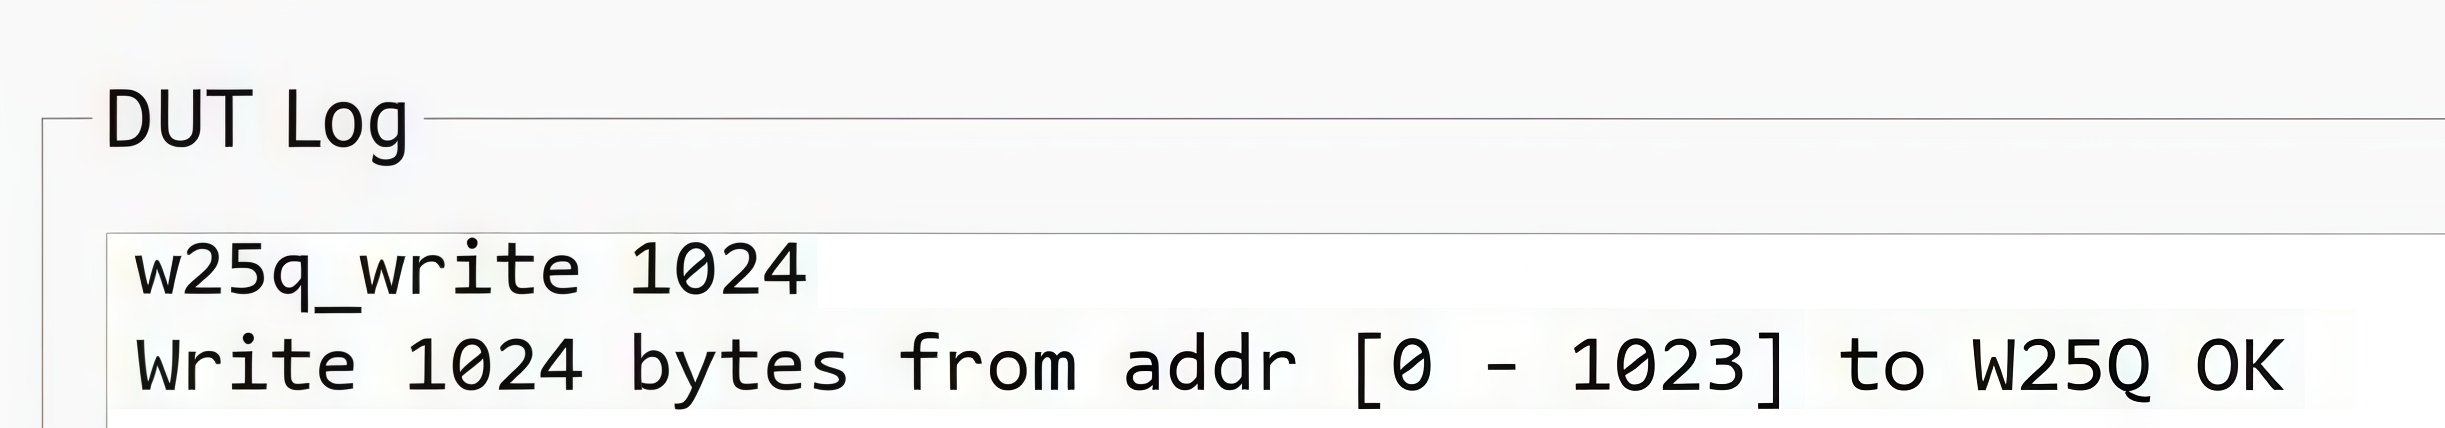
\includegraphics[width=0.8\textwidth]{image/spi_write.jpg}
        \caption{DUT ghi dữ liệu vào SPI Flash mô phỏng}
        \label{fig:spi_write}
    \end{figure}

    \item \textbf{Bước 5:} PC gửi lệnh đến \textbf{DUT}, yêu cầu DUT đọc vào vùng nhớ từ 0 - 1023. Dữ liệu đọc được sẽ được gửi lại PC để so sánh với dữ liệu DUT vừa ghi vào.
    \begin{figure}[H]
        \centering
        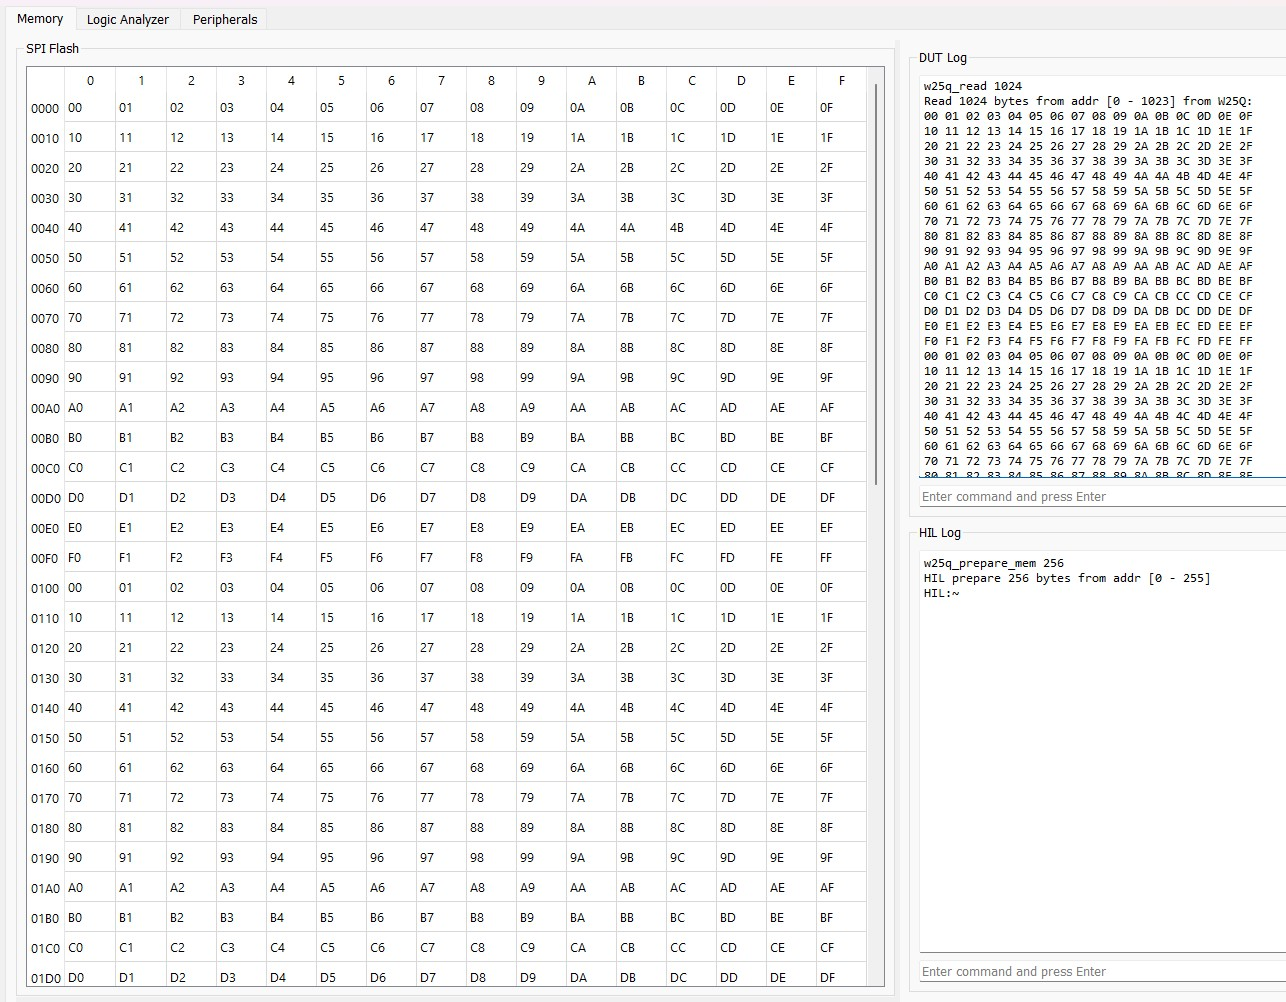
\includegraphics[width=1\textwidth]{image/spi_read_after_write.jpg}
        \caption{DUT đọc dữ liệu sau khi ghi vào SPI Flash mô phỏng}
        \label{fig:spi_read_after_write}
    \end{figure}

    \item \textbf{Bước 6:} PC gửi lệnh đến \textbf{DUT} xóa toàn bộ dữ liệu trên SPI Flash mô phỏng.\\
    \begin{figure}[H]
        \centering
        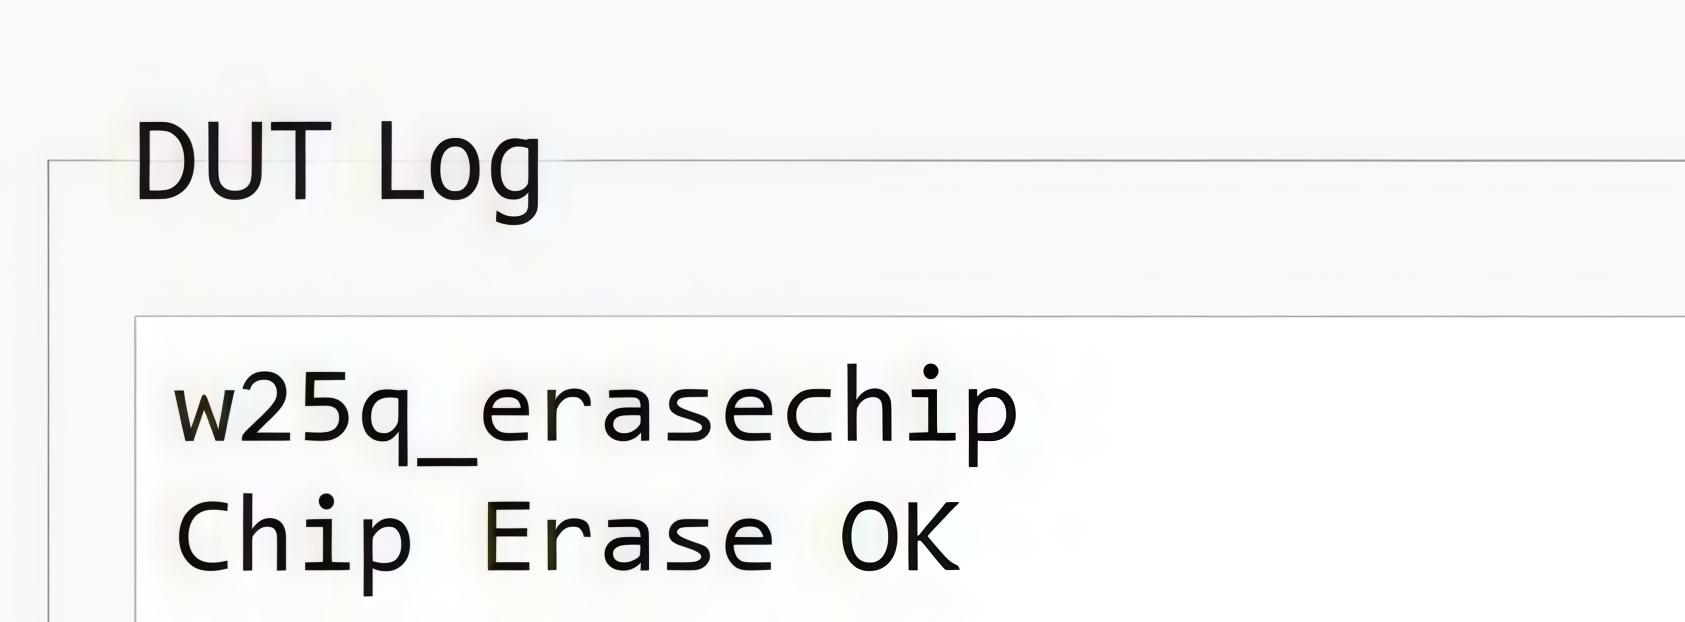
\includegraphics[width=0.65\textwidth]{image/spi_erase.jpg}
        \caption{DUT xóa dữ liệu trên SPI Flash mô phỏng}
        \label{fig:spi_erase}
    \end{figure}

    \item \textbf{Bước 7:} PC gửi lệnh đến \textbf{DUT}, yêu cầu DUT đọc vào vùng nhớ từ 0 - 1023 (toàn bộ giá trị đều là 0xFF sau khi xóa).
    \begin{figure}[H]
        \centering
        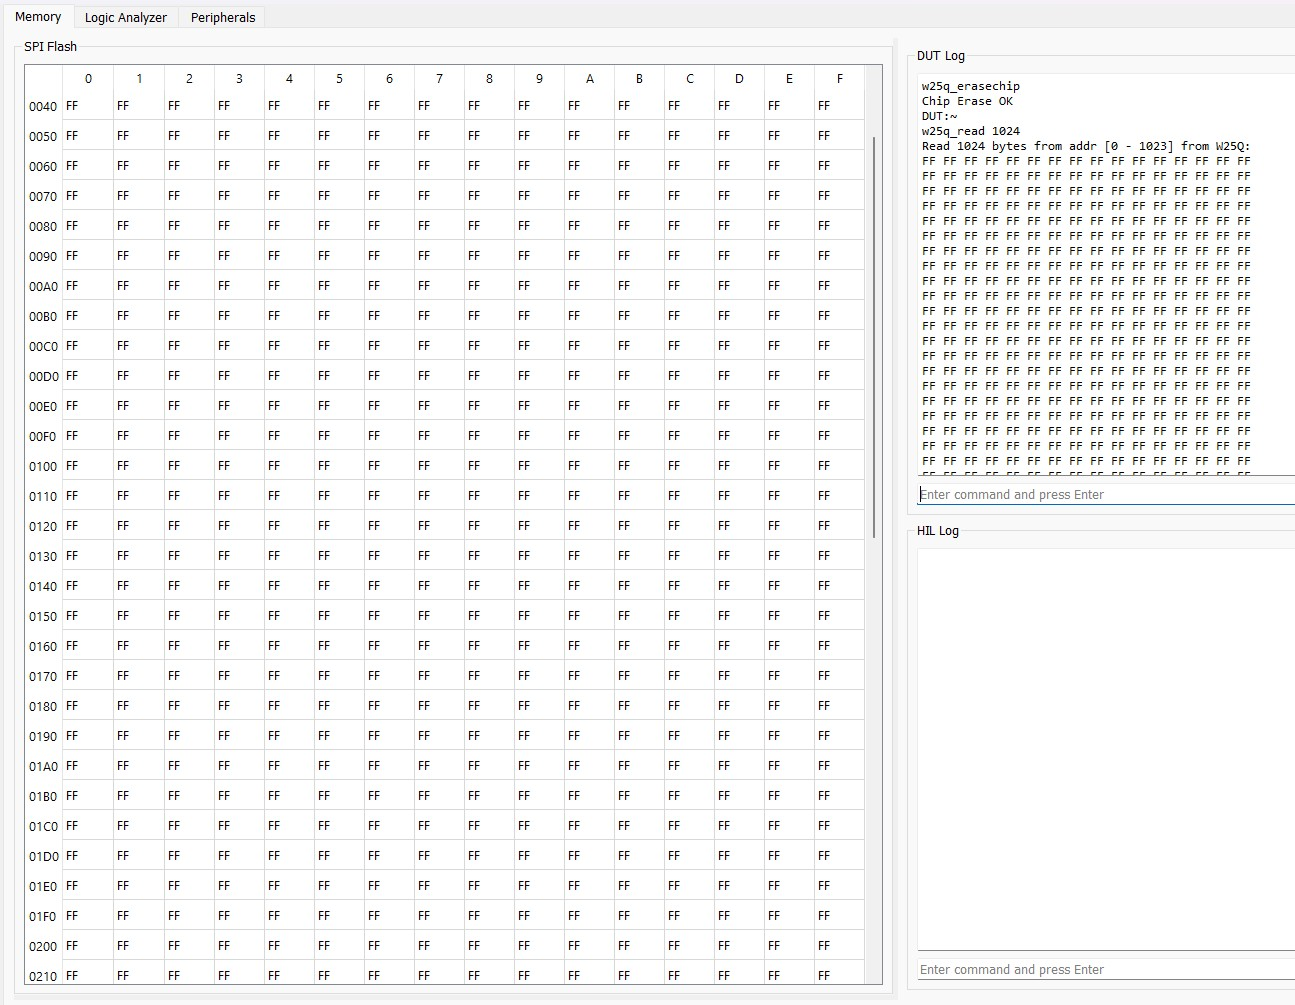
\includegraphics[width=1\textwidth]{image/spi_read_after_erase.jpg}
        \caption{DUT đọc dữ liệu sau khi xóa trên SPI Flash mô phỏng}
        \label{fig:spi_read_after_erase}
    \end{figure}
\end{itemize}

Sau khi hoàn thành các bước kiểm thử, kết quả sẽ được hiển thị trên giao diện chính của phần mềm PC như Hình \ref{fig:spi_test_result}.\\

\begin{figure}[H]
    \centering
    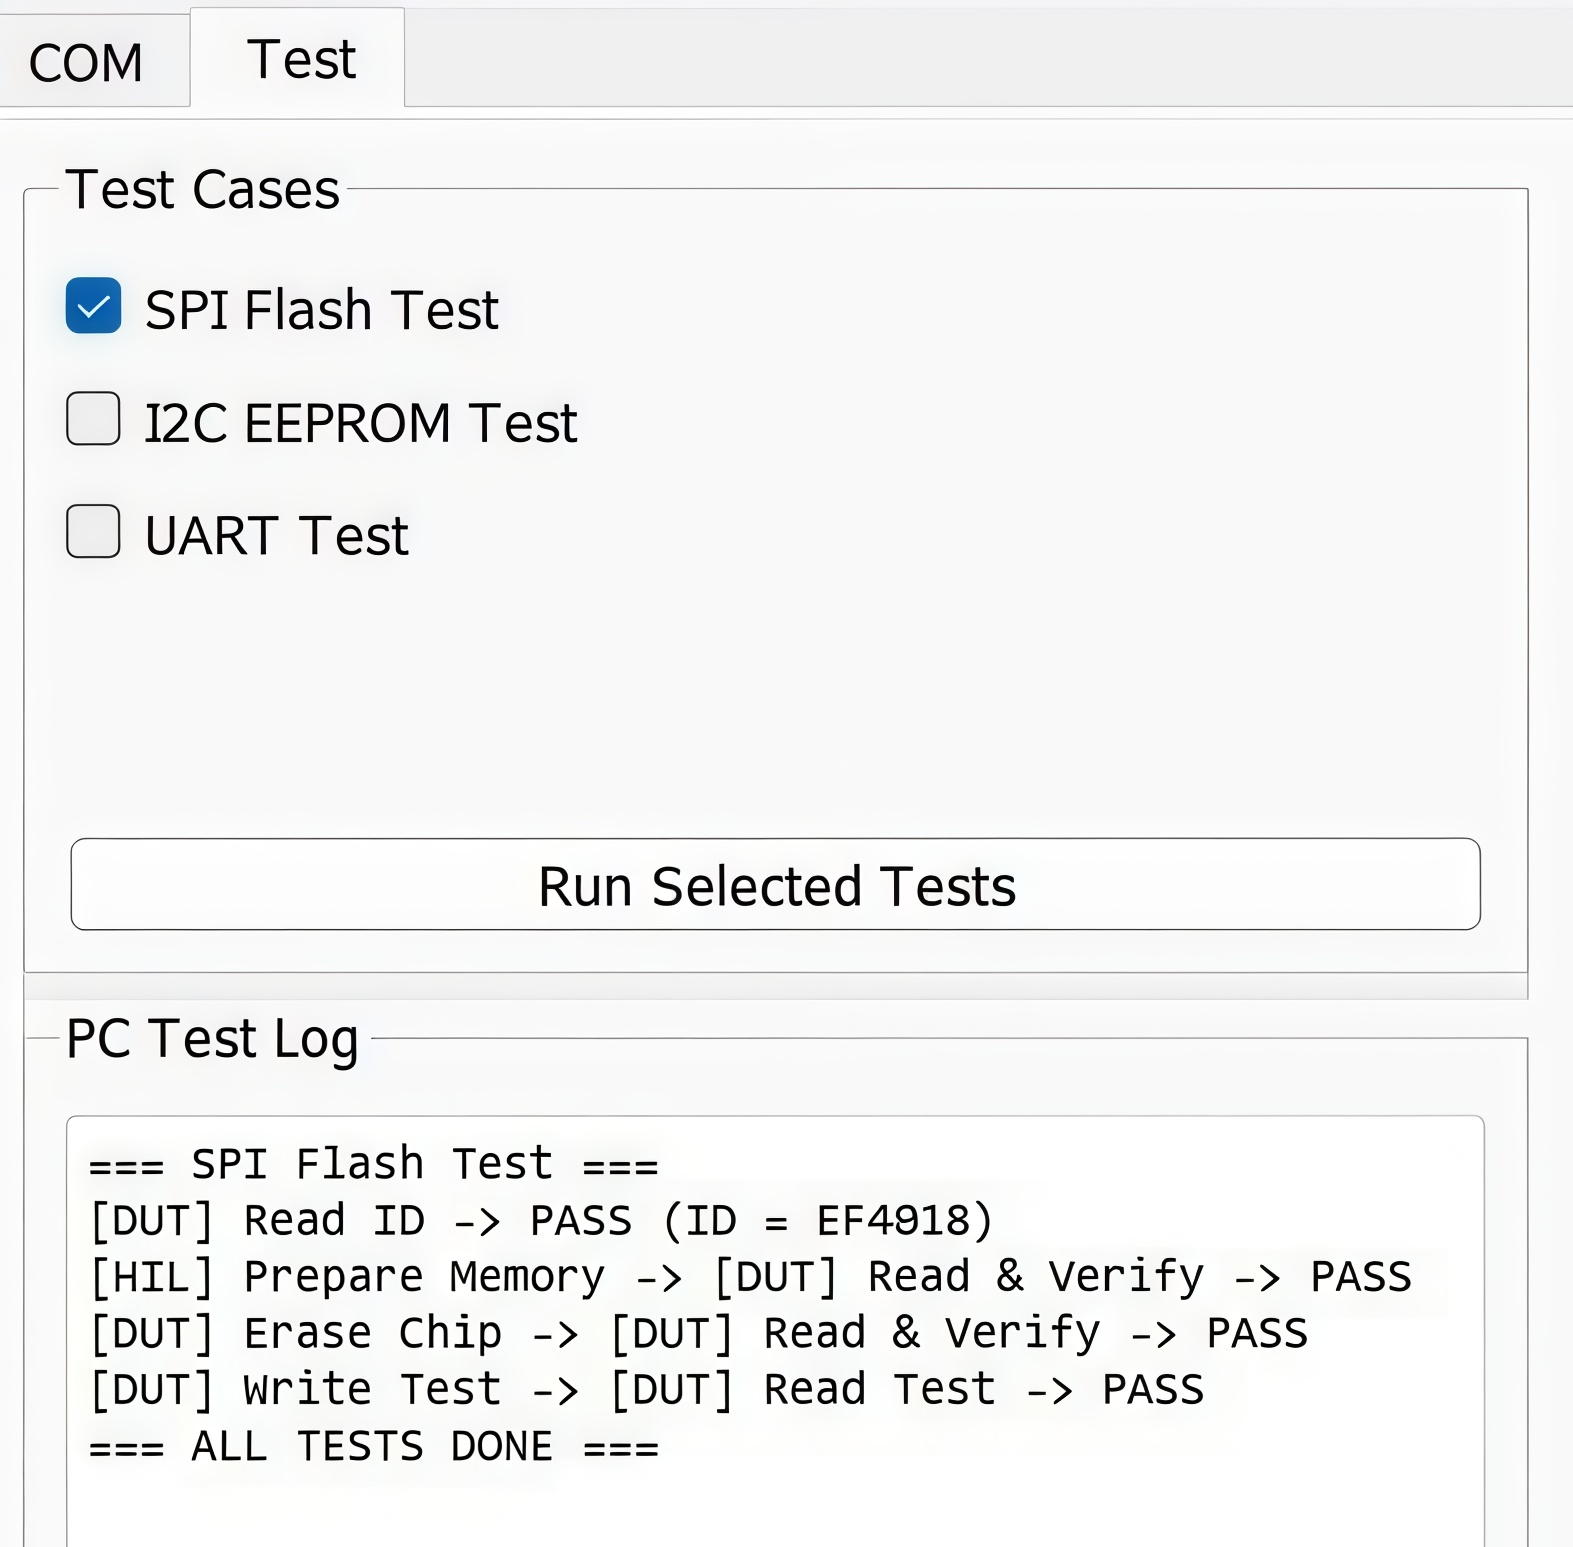
\includegraphics[width=0.7\textwidth]{image/spi_result.jpg}
    \caption{Kết quả kiểm thử SPI Flash trên phần mềm PC}
    \label{fig:spi_test_result}
\end{figure}
Kết quả kiểm thử cho thấy DUT đã thực hiện chính xác các thao tác đọc, ghi và xóa dữ liệu trên thiết bị SPI Flash mô phỏng bởi hệ thống HIL. 
Dữ liệu đọc được từ DUT hoàn toàn khớp với dữ liệu gốc đã được khởi tạo trên HIL, chứng tỏ tính đúng đắn của quá trình giao tiếp và xử lý dữ liệu giữa DUT và HIL.


\section{Kết quả thực hiện phần mềm kiểm thử tự động trên máy tính}

\subsection{Tổ chức thư mục}
Để thuận tiện cho việc phát triển, mở rộng và bảo trì hệ thống kiểm thử tự động, cấu trúc thư mục của dự án được tổ chức theo hướng phân tách rõ ràng giữa các thành phần kiểm thử, thư viện keyword, tài nguyên dùng chung và kết quả thực thi. 

Hệ thống kiểm thử được xây dựng dựa trên Robot Framework kết hợp với các thư viện Python nhằm hỗ trợ giao tiếp với HIL và Logic Analyzer. Cấu trúc thư mục tổng quát của hệ thống được trình bày như Hình \ref{fig:robot_folder_structure}.

\begin{figure}[H]
    \centering
    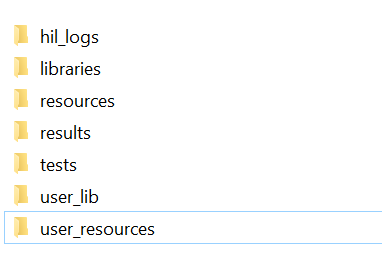
\includegraphics[width=0.8\textwidth]{image/robot_folder_structure.png}
    \caption{Lưu đồ giải thuật kiểm tra kết nối HIL và DUT}
    \label{fig:robot_folder_structure}
\end{figure}

Trong đó, các thư mục chính của hệ thống HIL bao gồm:

\begin{itemize}
    \item \textbf{hil\_logs/}: Ghi lại các log chi tiết của quá trình giao tiếp giữa Robot Framework với hệ thống HIL, bao gồm các lệnh đã gửi, phản hồi nhận được và trạng thái hoạt động của HIL trong suốt quá trình kiểm thử mỗi lần chạy.
    \item \textbf{libraries/}: Chứa các tập tin định nghĩa keyword dùng chung trong Robot Framework. Các keyword này được sử dụng để xây dựng các bước kiểm thử ở mức cao, giúp test case trở nên trực quan và thân thiện với người dùng hơn. Các thư viện này cũng đóng vai trò là lớp giao tiếp trung gian giữa Robot Framework với hệ thống HIL và Logic Analyzer, giúp ẩn đi các chi tiết mức thấp và cung cấp các thao tác đơn giản để điều khiển hệ thống.
    \item \textbf{resources/}: Chứa các tài nguyên dùng chung như biến cấu hình, thông số giao tiếp,... cho HIL, được sử dụng trong nhiều bài kiểm thử khác nhau.
    \item \textbf{results/}: Chứa kết quả sau khi thực hiện kiểm thử bao gồm file báo cáo tổng hợp, file log chi tiết và các dữ liệu phục vụ cho việc đánh giá kết quả kiểm thử.
    \item \textbf{tests/}: Chứa các tập tin kiểm thử được xây dựng bằng Robot Framework. Hệ thống hiện đã cung cấp sẵn các bài kiểm thử mẫu cho các ngoại vi và thiết bị mô phỏng được hỗ trợ trên HIL nhằm giúp người dùng tham khảo và phát triển thêm các kịch bản kiểm thử mới.

\end{itemize}

Các thư mục do người dùng tạo ra bao gồm:

\begin{itemize}
    \item \textbf{user\_lib/}: Chứa các tập tin định nghĩa keyword do người dùng tự định nghĩa để giao tiếp với hệ thống DUT.
    \item \textbf{user\_resources/}: Chứa các tài nguyên dùng chung như biến cấu hình, thông số giao tiếp,... cho DUT, được sử dụng trong nhiều bài kiểm thử khác nhau.

\end{itemize}

Với cách tổ chức này, các thành phần trong hệ thống được phân tách rõ ràng giữa phần kiểm thử, phần xử lý giao tiếp phần cứng và phần kết quả đầu ra. Điều này giúp việc phát triển thêm các bài kiểm thử mới, mở rộng hỗ trợ cho các ngoại vi khác cũng như tái sử dụng framework cho nhiều DUT khác nhau trở nên thuận tiện hơn.

\subsection{Các keyword hỗ trợ trong hệ thống kiểm thử}

Các keyword được xây dựng trong hệ thống kiểm thử tự động đóng vai trò là lớp giao tiếp trung gian giữa Robot Framework với hệ thống HIL và Logic Analyzer. Thay vì thao tác trực tiếp với các lệnh điều khiển mức thấp, người phát triển chỉ cần sử dụng các keyword tương ứng để xây dựng các test case theo dạng mô tả hành vi kiểm thử.

Bảng \ref{tab:hil_keywords} và Bảng \ref{tab:la_keywords} trình bày các keyword tiêu biểu được hỗ trợ trong hệ thống kiểm thử.

\renewcommand{\arraystretch}{1.3}

\begin{longtable}{|p{4.8cm}|p{8.7cm}|}
\caption{Các keyword hỗ trợ bởi thư viện HIL}
\label{tab:hil_keywords} \\

\hline
\textbf{Keyword} & \textbf{Chức năng} \\
\hline
\endfirsthead

\hline
\textbf{Keyword} & \textbf{Chức năng} \\
\hline
\endhead

\multicolumn{2}{|c|}{\textbf{Kết nối và điều khiển DUT}} \\
\hline

Connect HIL
& Thiết lập kết nối giữa PC và hệ thống HIL thông qua USB serial. \\
\hline

Disconnect HIL
& Ngắt kết nối giữa PC và hệ thống HIL. \\
\hline

Verify HIL Alive
& Kiểm tra khả năng phản hồi và trạng thái hoạt động của HIL. \\
\hline

HIL Power DUT On
& Cấp nguồn cho DUT thông qua HIL. \\
\hline

HIL Power DUT Off
& Ngắt nguồn DUT thông qua HIL. \\
\hline

HIL Power DUT Cycle
& Thực hiện reset nguồn DUT bằng cách tắt và cấp nguồn lại. \\
\hline

HIL Flash Firmware for DUT
& Nạp firmware cho DUT thông qua chế độ DFU sử dụng STM32CubeProgrammer CLI. \\
\hline

\multicolumn{2}{|c|}{\textbf{GPIO}} \\
\hline

HIL Set GPIO
& Thiết lập trạng thái logic cho chân GPIO mô phỏng. \\
\hline

HIL Read GPIO
& Đọc trạng thái logic của chân GPIO từ DUT. \\
\hline

\multicolumn{2}{|c|}{\textbf{UART}} \\
\hline

HIL Init UART
& Khởi tạo giao tiếp UART trên HIL. \\
\hline

HIL Send UART String
& Gửi chuỗi dữ liệu UART đến DUT. \\
\hline

HIL Read UART Data
& Đọc dữ liệu UART phản hồi từ DUT. \\
\hline

HIL Verify UART String
& Kiểm tra tính đúng đắn của chuỗi UART nhận được. \\
\hline

\multicolumn{2}{|c|}{\textbf{CAN}} \\
\hline

HIL Send CAN Buffer
& Gửi dữ liệu CAN dạng buffer đến DUT. \\
\hline

HIL Send CAN String
& Gửi chuỗi dữ liệu thông qua giao tiếp CAN. \\
\hline

HIL Read CAN Data
& Đọc dữ liệu phản hồi từ giao tiếp CAN. \\
\hline

HIL Verify CAN String Data
& Kiểm tra tính đúng đắn của chuỗi dữ liệu CAN nhận được. \\
\hline

\multicolumn{2}{|c|}{\textbf{I2C EEPROM}} \\
\hline

HIL Init EEPROM
& Khởi tạo EEPROM mô phỏng trên bus I2C. \\
\hline

HIL Deinit EEPROM
& Giải phóng EEPROM mô phỏng khỏi hệ thống HIL. \\
\hline

HIL Find EEPROM
& Kiểm tra sự tồn tại của EEPROM trên bus I2C. \\
\hline

HIL Activate I2C Device
& Kích hoạt thiết bị I2C mô phỏng trên HIL. \\
\hline

\multicolumn{2}{|c|}{\textbf{I2C RTC}} \\
\hline

HIL Init RTC
& Khởi tạo RTC mô phỏng trên bus I2C. \\
\hline

HIL Prepare RTC Time
& Thiết lập thời gian cho RTC mô phỏng. \\
\hline

HIL Get RTC Time
& Đọc giá trị thời gian hiện tại từ RTC mô phỏng. \\
\hline

HIL Set RTC Date
& Thiết lập ngày tháng cho RTC mô phỏng. \\
\hline

HIL Get RTC Date
& Đọc ngày tháng hiện tại từ RTC mô phỏng. \\
\hline

\multicolumn{2}{|c|}{\textbf{SPI Flash}} \\
\hline

HIL Prepare SPI Flash Data
& Chuẩn bị dữ liệu mẫu trong SPI Flash để DUT thực hiện đọc dữ liệu. \\
\hline

\multicolumn{2}{|c|}{\textbf{ADC/DAC}} \\
\hline

HIL Read ADC Voltage
& Đọc giá trị điện áp ADC đo được từ HIL. \\
\hline

HIL Set DAC Voltage
& Thiết lập điện áp DAC đầu ra của HIL. \\
\hline

HIL Generate Sine Wave
& Tạo tín hiệu sine wave phục vụ kiểm thử DAC hoặc ADC. \\
\hline

HIL Stop Sine Wave
& Dừng phát tín hiệu sine wave. \\
\hline

HIL Generate Triangle Wave
& Tạo tín hiệu triangle wave phục vụ kiểm thử DAC hoặc ADC. \\
\hline

HIL Stop Triangle Wave
& Dừng phát tín hiệu triangle wave. \\
\hline

\end{longtable}

\begin{table}[H]
\centering
\caption{Các keyword hỗ trợ bởi thư viện Logic Analyzer}
\label{tab:la_keywords}
\renewcommand{\arraystretch}{1.3}

\begin{tabular}{|p{5cm}|p{8.5cm}|}
\hline
\textbf{Keyword} & \textbf{Chức năng} \\
\hline

Connect Logic Analyzer
& Thiết lập kết nối với Logic Analyzer thông qua USB serial. \\
\hline

Disconnect Logic Analyzer
& Ngắt kết nối với Logic Analyzer. \\
\hline

LA Read Data
& Thu thập dữ liệu tín hiệu từ Logic Analyzer. \\
\hline

LA Verify Sine Wave
& Phân tích FFT để xác minh tín hiệu analog dạng sine wave và kiểm tra tần số tín hiệu. \\
\hline

LA Verify Pulse Wave
& Phân tích tín hiệu số nhằm xác định tần số và duty cycle của tín hiệu PWM hoặc pulse wave. \\
\hline

LA Verify Triangle Wave
& Phân tích phổ hài để xác minh tín hiệu analog dạng triangle wave. \\
\hline

\end{tabular}
\end{table}

\subsection{Ví dụ test case kiểm thử}

Trong Robot Framework, một tập tin kiểm thử được tổ chức thành nhiều thành phần nhằm mô tả tài nguyên sử dụng, biến cấu hình và các bước kiểm thử. Việc tổ chức theo cấu trúc này giúp các bài kiểm thử trở nên trực quan, dễ mở rộng và thuận tiện cho việc tái sử dụng trong nhiều dự án khác nhau.

Để minh họa cho cách xây dựng một bài kiểm thử trong hệ thống, luận văn sử dụng ví dụ kiểm thử chức năng đọc điện áp ADC của DUT thông qua tín hiệu DAC được tạo bởi HIL. Nội dung file kiểm thử được trình bày như Hình \ref{fig:robot_adc_testcase}.

\begin{figure}[H]
    \centering
    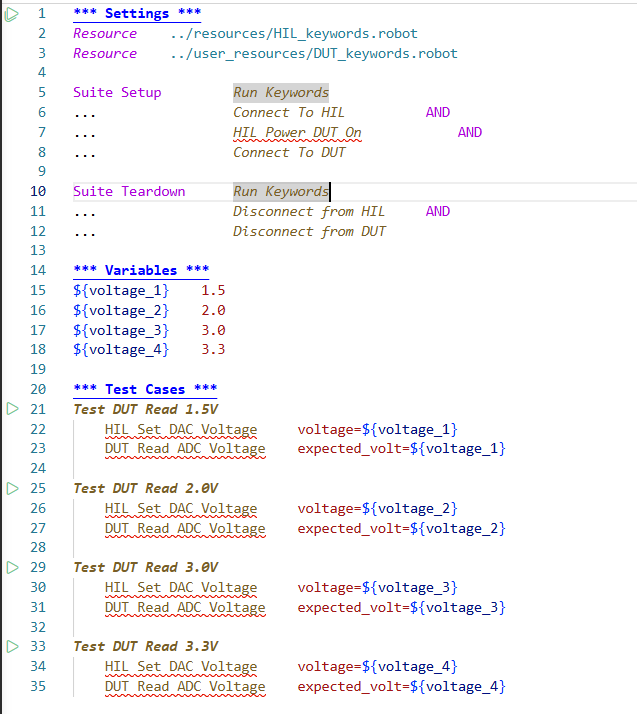
\includegraphics[width=0.8\textwidth]{image/robot_adc_testcase.png}
    \caption{í dụ file kiểm thử ADC bằng Robot Framework}
    \label{fig:robot_adc_testcase}
\end{figure}

Trong Robot Framework, phần \textbf{Settings} được sử dụng để khai báo các tài nguyên, thư viện và cấu hình chung cho toàn bộ file kiểm thử. 

Trong ví dụ trên, hai dòng lệnh:

\begin{lstlisting}[language={}]
Resource    ../resources/HIL_keywords.robot
Resource    ../user_resources/DUT_keywords.robot
\end{lstlisting}

được sử dụng để import các tập tin resource chứa các keyword phục vụ cho quá trình kiểm thử.

Trong đó:

\begin{itemize}

    \item \textbf{HIL\_keywords.robot}: Chứa các keyword phục vụ điều khiển hệ thống HIL như điều khiển DAC, GPIO, UART, CAN hoặc các thiết bị mô phỏng ngoại vi.

    \item \textbf{DUT\_keywords.robot}: Chứa các keyword do người dùng xây dựng để giao tiếp và kiểm tra DUT, ví dụ như đọc dữ liệu UART từ DUT hoặc xác minh giá trị ADC mà DUT đo được.

\end{itemize}

Việc tách các keyword thành các file resource riêng giúp tăng khả năng tái sử dụng và giảm sự phụ thuộc trực tiếp giữa các test case với phần xử lý giao tiếp mức thấp.

Ngoài ra, phần \textbf{Settings} còn định nghĩa các bước khởi tạo và giải phóng tài nguyên thông qua \textit{Suite Setup} và \textit{Suite Teardown}.

\begin{itemize}

    \item \textbf{Suite Setup}: Là tập hợp các thao tác được thực hiện một lần trước khi bắt đầu chạy toàn bộ các test case trong file kiểm thử.

\end{itemize}

Trong ví dụ trên, \textit{Suite Setup} thực hiện các bước:

\begin{enumerate}

    \item Thiết lập kết nối giữa máy tính và hệ thống HIL.
    
    \item Cấp nguồn cho DUT thông qua HIL.
    
    \item Thiết lập kết nối giao tiếp với DUT.

\end{enumerate}

Nhờ đó, toàn bộ môi trường kiểm thử được chuẩn bị tự động trước khi thực hiện các bài kiểm thử.

\begin{itemize}

    \item \textbf{Suite Teardown}: Là tập hợp các thao tác được thực hiện sau khi hoàn thành toàn bộ quá trình kiểm thử nhằm giải phóng tài nguyên và đưa hệ thống về trạng thái an toàn.

\end{itemize}

Trong ví dụ trên, \textit{Suite Teardown} thực hiện đóng kết nối với HIL và DUT sau khi tất cả các test case đã chạy xong.

Phần \textbf{Variables} được sử dụng để khai báo các biến dùng chung trong file kiểm thử. Các giá trị điện áp như 1.5V, 2.0V, 3.0V và 3.3V được lưu dưới dạng biến nhằm giúp việc thay đổi tham số kiểm thử trở nên thuận tiện hơn và tăng khả năng tái sử dụng test case.

Phần \textbf{Test Cases} chứa các kịch bản kiểm thử cụ thể. Mỗi test case trong ví dụ trên thực hiện quy trình kiểm thử ADC của DUT theo các bước:

\begin{enumerate}

    \item HIL phát ra mức điện áp tương ứng thông qua DAC.
    
    \item DUT thực hiện đọc giá trị điện áp bằng ADC.
    
    \item DUT gửi kết quả đo được về máy tính.
    
    \item Keyword kiểm thử thực hiện so sánh giá trị nhận được với giá trị mong đợi để xác định kết quả đạt hoặc không đạt.

\end{enumerate}

\subsection{Quy trình thực hiện kiểm thử tự động}
\subsubsection{Thực hiện một bài kiểm thử}

Đối với một bài kiểm thử đơn lẻ, người dùng có thể thực hiện chạy trực tiếp file test case bằng lệnh Robot Framework tương ứng.

Ví dụ:

\begin{lstlisting}[language=bash]
robot -d results .\tests\05__analog_test.robot
\end{lstlisting}

Sau khi thực thi lệnh, Robot Framework sẽ tự động:

\begin{itemize}

    \item Phân tích file kiểm thử.
    
    \item Import các resource và keyword cần thiết.
    
    \item Thực hiện các bước trong \textit{Suite Setup}.
    
    \item Chạy lần lượt các test case trong file.
    
    \item Đánh giá kết quả đạt hoặc không đạt.
    
    \item Thực hiện \textit{Suite Teardown}.
    
    \item Sinh báo cáo kiểm thử sau khi hoàn thành.

\end{itemize}

Trong quá trình thực hiện, trạng thái của từng test case sẽ được hiển thị trực tiếp trên terminal nhằm hỗ trợ người dùng theo dõi tiến trình kiểm thử.

\begin{figure}[H]
    \centering
    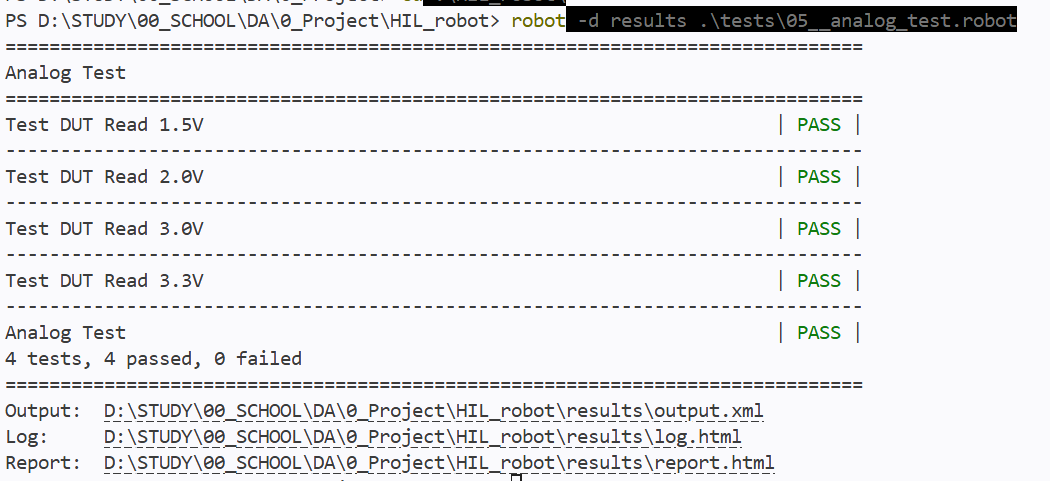
\includegraphics[width=0.85\textwidth]{image/robot_terminal.png}
    \caption{Trạng thái thực hiện kiểm thử được hiển thị trên terminal}
    \label{fig:robot_terminal}
\end{figure}

\subsubsection{Thực hiện nhiều bài kiểm thử liên tiếp}

Ngoài việc thực hiện một bài kiểm thử đơn lẻ, hệ thống còn hỗ trợ chạy nhiều file kiểm thử liên tiếp nhằm phục vụ cho kiểm thử hồi quy firmware.

Người dùng có thể thực hiện kiểm thử toàn bộ thư mục chứa các test case bằng lệnh:

\begin{lstlisting}[language=bash]
robot -d results .\tests\
\end{lstlisting}

Khi đó, Robot Framework sẽ tự động tìm kiếm tất cả các file kiểm thử trong thư mục \textit{tests/} và thực hiện tuần tự từng bài kiểm thử.

Cơ chế này cho phép:

\begin{itemize}

    \item Kiểm thử đồng thời nhiều chức năng của DUT.
    
    \item Tự động hóa quá trình kiểm thử firmware sau mỗi lần cập nhật.
    
    \item Giảm thời gian thao tác thủ công của người phát triển.
    
    \item Hỗ trợ kiểm thử hồi quy nhằm phát hiện lỗi phát sinh sau khi thay đổi firmware.

\end{itemize}

Sau khi hoàn thành, Robot Framework sẽ tự động tổng hợp kết quả của toàn bộ các bài kiểm thử và sinh báo cáo thống kê tổng quát.

\subsubsection{Thiết lập thứ tự thực hiện các bài kiểm thử}

Trong một số trường hợp, các bài kiểm thử cần được thực hiện theo một trình tự xác định nhằm đảm bảo trạng thái hoạt động phù hợp của DUT hoặc phục vụ cho quá trình kiểm thử hồi quy.

Để hỗ trợ điều này, hệ thống cho phép người dùng tổ chức thứ tự thực hiện test case theo nhiều phương pháp khác nhau.

Một phương pháp đơn giản là sử dụng tiền tố số thứ tự (\textit{numeric prefix}) trong tên file kiểm thử. Ví dụ:

\begin{lstlisting}[language={}]
tests/
|-- 01_gpio.robot
|-- 02_adc.robot
|-- 03_uart.robot
|-- 04_can.robot
\end{lstlisting}

Khi thực hiện chạy toàn bộ thư mục kiểm thử, Robot Framework sẽ thực hiện các file theo thứ tự tên file, từ đó đảm bảo đúng trình tự kiểm thử mong muốn.

Ngoài ra, hệ thống cũng hỗ trợ xây dựng một file điều phối kiểm thử dùng để quy định rõ trình tự thực hiện các bài kiểm thử. File này đóng vai trò như một tập kiểm thử tổng hợp (\textit{test suite}) dùng để gọi lần lượt các test case hoặc các nhóm kiểm thử khác nhau.

Phương pháp này phù hợp với các hệ thống có số lượng bài kiểm thử lớn hoặc cần xây dựng các kịch bản kiểm thử chuyên biệt cho từng phiên bản firmware.

Nhờ khả năng tổ chức linh hoạt này, người dùng có thể dễ dàng quản lý quá trình kiểm thử tự động, đồng thời đảm bảo các bài kiểm thử được thực hiện theo đúng trình tự yêu cầu của hệ thống.

\subsection{Kết quả sinh báo cáo}

Sau khi hoàn thành quá trình kiểm thử tự động, Robot Framework sẽ tự động sinh ra các tập tin báo cáo phục vụ cho việc theo dõi, phân tích và đánh giá kết quả kiểm thử.

Các tập tin kết quả được lưu trong thư mục \textit{results/} của hệ thống kiểm thử. Trong đó, các tập tin quan trọng bao gồm:

\begin{itemize}

    \item \textbf{report.html}: Báo cáo tổng hợp kết quả kiểm thử.
    
    \item \textbf{log.html}: File log chi tiết quá trình thực hiện từng keyword và test case.
    
    \item \textbf{output.xml}: File dữ liệu kết quả ở định dạng XML phục vụ cho việc lưu trữ hoặc tích hợp với các hệ thống CI/CD trong tương lai.
\end{itemize}

Hình \ref{fig:robot_report_success} trình bày giao diện báo cáo khi toàn bộ bài kiểm thử thực hiện thành công.

\begin{figure}[H]
    \centering
    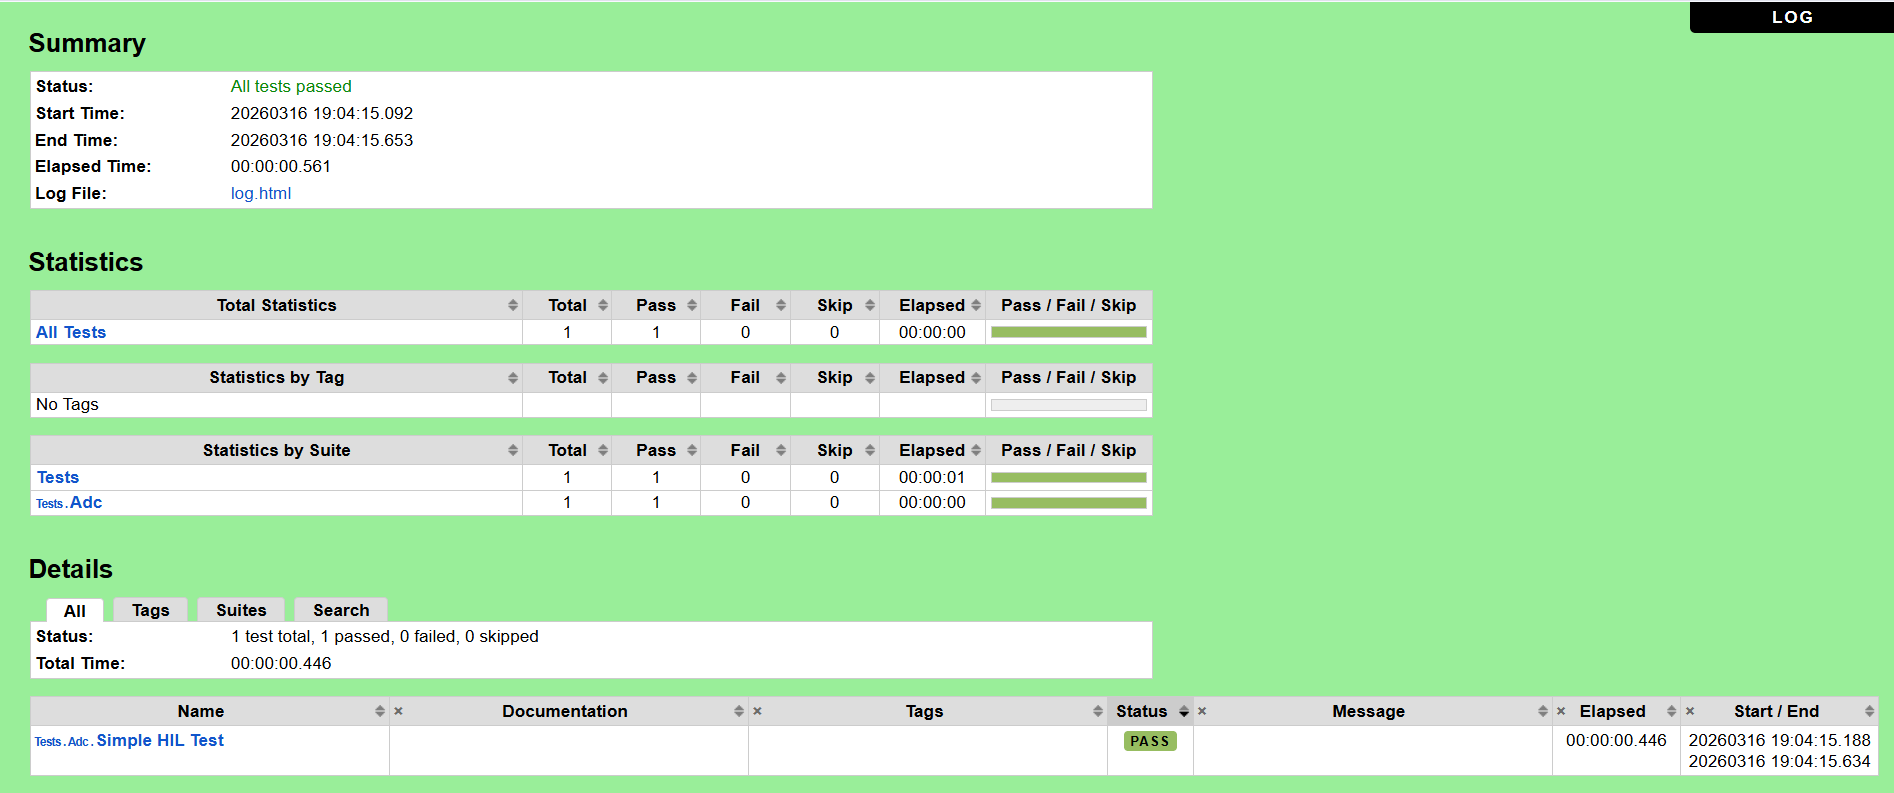
\includegraphics[width=0.85\textwidth]{image/robot_report_success.png}
    \caption{Báo cáo kiểm thử khi toàn bộ test case đạt}
    \label{fig:robot_report_success}
\end{figure}

Trong trường hợp tất cả các điều kiện kiểm thử đều thỏa mãn, Robot Framework sẽ đánh dấu trạng thái \textit{PASS} cho từng test case cũng như toàn bộ test suite. Báo cáo đồng thời cung cấp thông tin về:

\begin{itemize}
    \item Số lượng test case đạt và không đạt.
    \item Thời gian thực hiện kiểm thử.
    \item Tỷ lệ thành công của toàn bộ bài kiểm thử.
    \item Tên các test case đã thực hiện.
\end{itemize}

Ngược lại, khi xuất hiện lỗi trong quá trình kiểm thử hoặc kết quả đo được không đúng với giá trị mong đợi, Robot Framework sẽ đánh dấu trạng thái \textit{FAIL}. Ví dụ báo cáo khi bài kiểm thử thất bại được trình bày như Hình \ref{fig:robot_report_fail}.

\begin{figure}[H]
    \centering
    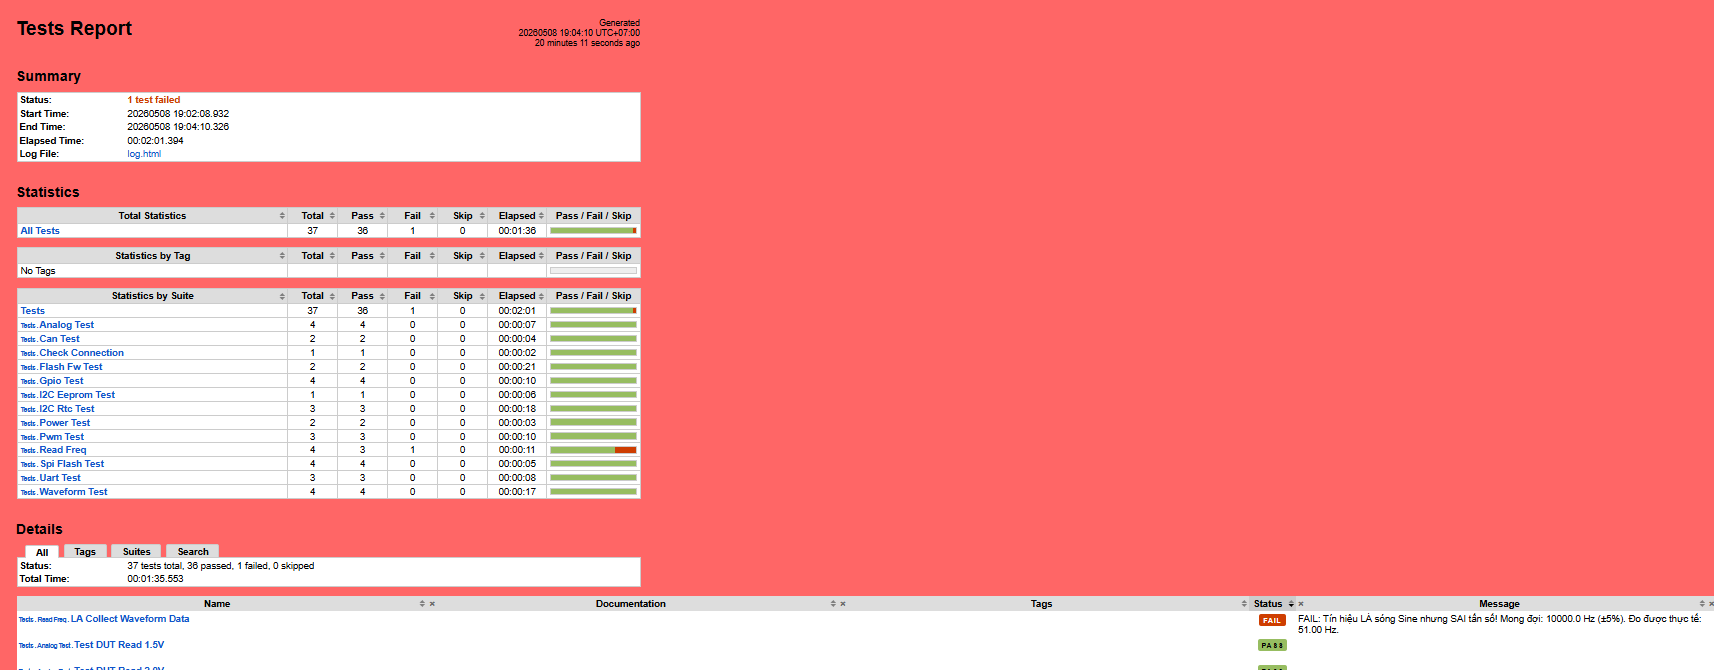
\includegraphics[width=0.85\textwidth]{image/robot_report_fail.png}
    \caption{Báo cáo kiểm thử khi toàn bộ test case không đạt}
    \label{fig:robot_report_fail}
\end{figure}

Thông qua báo cáo này, người phát triển có thể nhanh chóng xác định test case xảy ra lỗi và tiến hành phân tích nguyên nhân.

Ngoài báo cáo tổng hợp, hệ thống còn sinh file \textit{log.html} nhằm ghi lại chi tiết toàn bộ quá trình thực hiện kiểm thử. Nội dung file log được trình bày như Hình \ref{fig:robot_log_file}.

\begin{figure}[H]
    \centering
    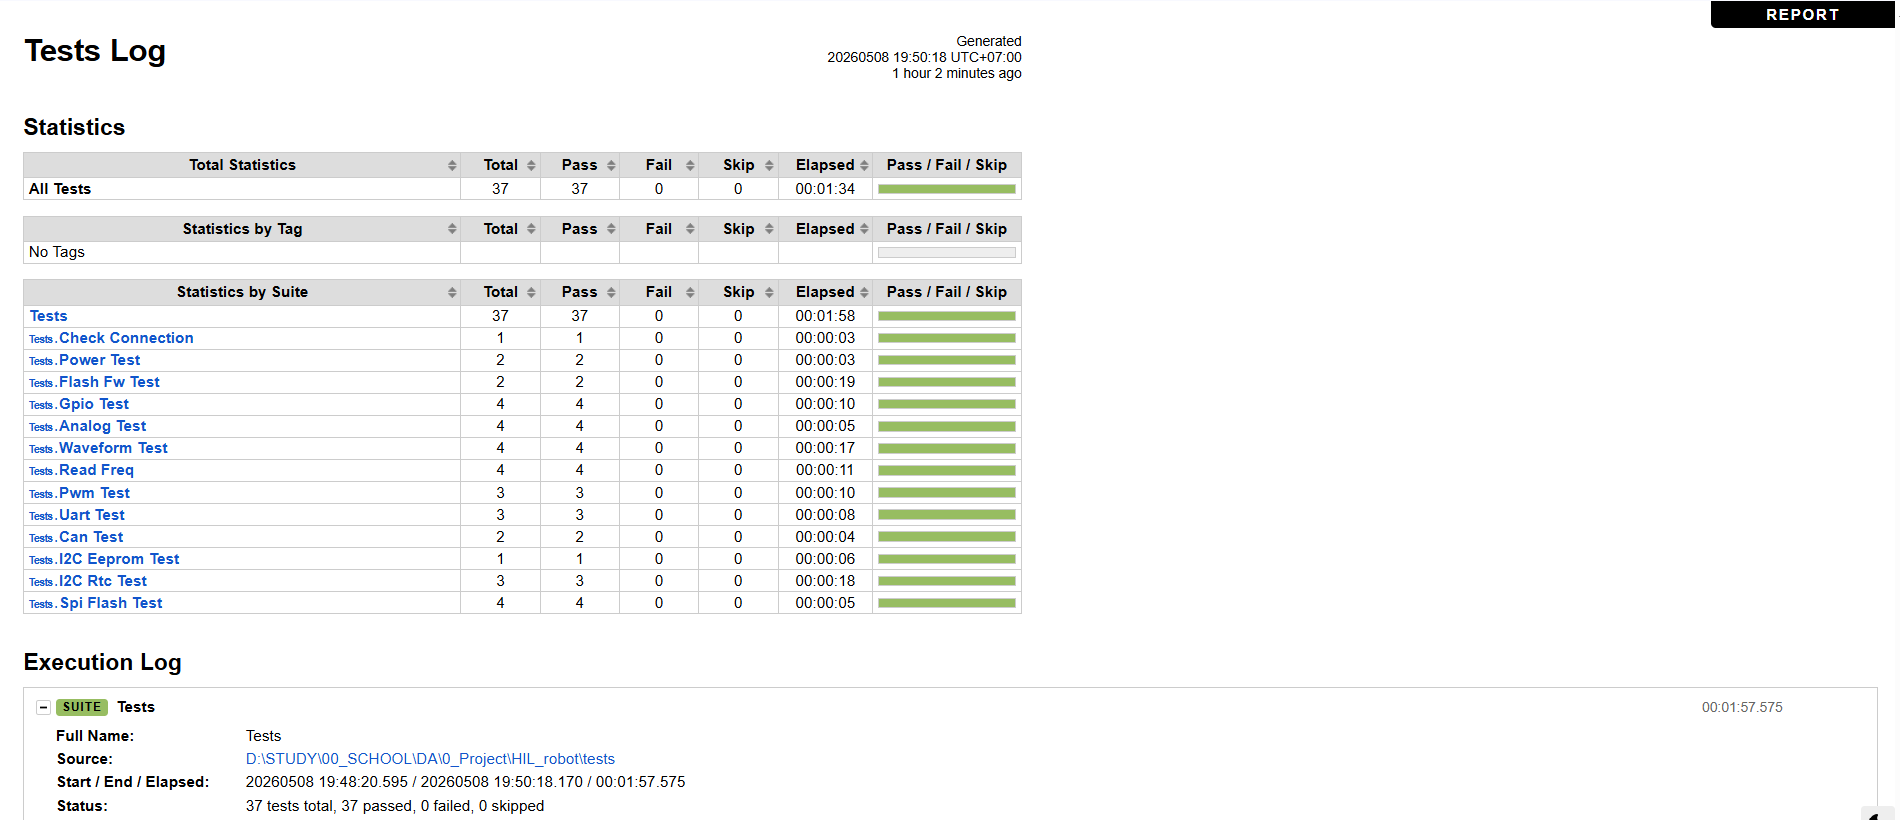
\includegraphics[width=0.85\textwidth]{image/robot_log.png}
    \caption{File log chi tiết của Robot Framework}
    \label{fig:robot_log_file}
\end{figure}

File log cung cấp thông tin chi tiết cho từng bước thực hiện bao gồm:

\begin{itemize}
    \item Các keyword đã được gọi.
    \item Tham số đầu vào của keyword.
    \item Dữ liệu phản hồi từ DUT hoặc HIL.
    \item Thời gian thực hiện từng bước.
    \item Thông báo lỗi và nguyên nhân gây lỗi nếu có.
\end{itemize}

Nhờ đó, người phát triển có thể dễ dàng theo dõi luồng thực thi của hệ thống và hỗ trợ quá trình phân tích lỗi firmware.

Bên cạnh đó, Robot Framework cũng sinh file \textit{output.xml} chứa toàn bộ kết quả kiểm thử ở dạng dữ liệu có cấu trúc. Ví dụ file \textit{output.xml} được trình bày như Hình \ref{fig:robot_output_xml}.

\begin{figure}[H]
    \centering
    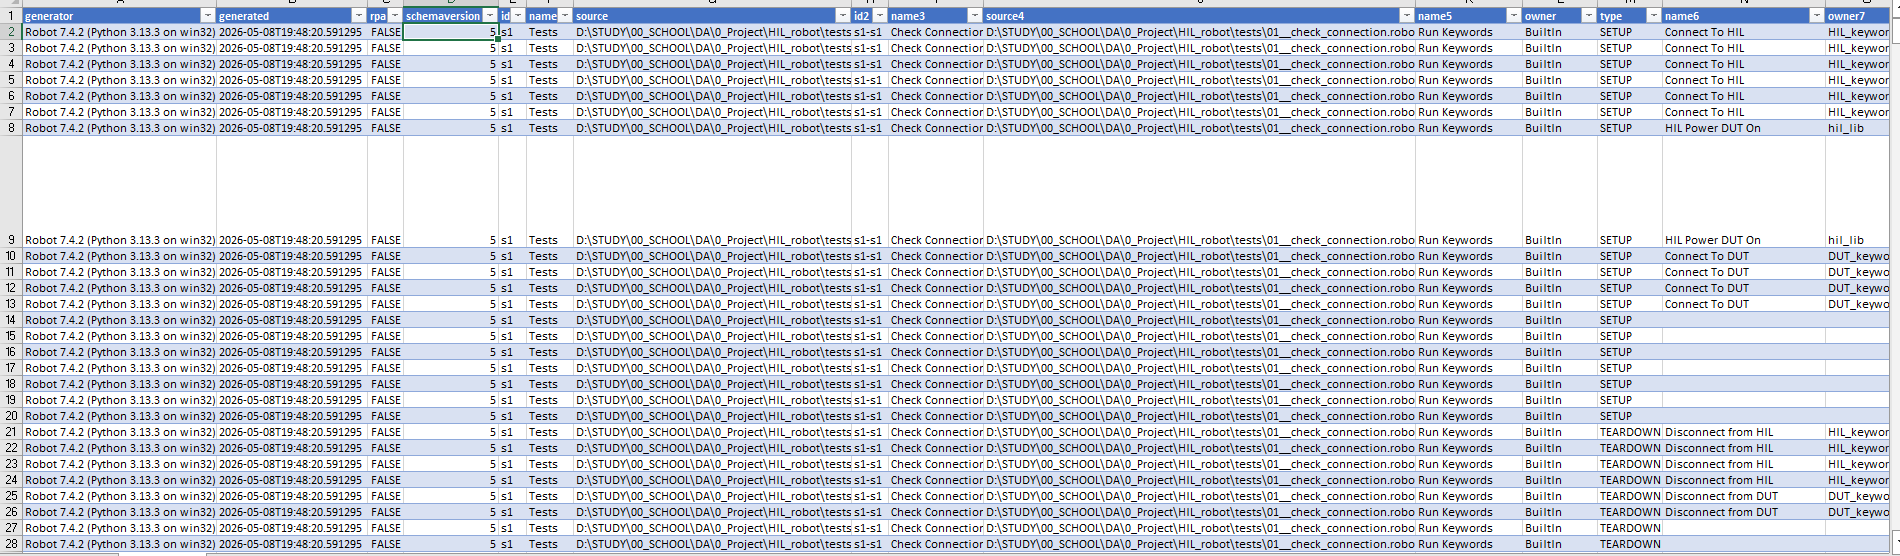
\includegraphics[width=0.85\textwidth]{image/robot_output.png}
    \caption{File output.xml chứa kết quả kiểm thử}
    \label{fig:robot_output_xml}
\end{figure}

File XML này cho phép hệ thống dễ dàng tích hợp với các công cụ xử lý kết quả kiểm thử hoặc các nền tảng tự động hóa khác trong tương lai như hệ thống CI/CD hoặc dashboard giám sát kiểm thử.

\subsubsection{File log giao tiếp HIL}

Ngoài các báo cáo của Robot Framework, hệ thống còn tự động ghi lại toàn bộ quá trình giao tiếp giữa máy tính và HIL thông qua file log serial với định dạng:

\begin{center}
\textbf{hil\_serial\_<ngày\_giờ>.log}
\end{center}

File log này lưu lại các lệnh điều khiển đã gửi đến HIL, dữ liệu phản hồi từ firmware cũng như trạng thái hoạt động của các ngoại vi mô phỏng trong suốt quá trình kiểm thử. Các file log này được lưu trong thư mục \textit{hil\_logs/} của hệ thống nhằm hỗ trợ người phát triển theo dõi và phân tích chi tiết quá trình giao tiếp với HIL.

Ví dụ, khi thực hiện kiểm thử CAN, file log sẽ ghi lại quá trình gửi dữ liệu CAN buffer, phản hồi nhận được từ DUT cũng như dữ liệu truyền nhận thực tế trên bus CAN. Tương tự, đối với các bài kiểm thử ADC, UART, GPIO hoặc I2C, file log cũng lưu lại toàn bộ nội dung giao tiếp tương ứng.

Hình \ref{fig:hil_serial_log} trình bày một phần nội dung của file log giao tiếp giữa Robot Framework và HIL.

\begin{figure}[H]
    \centering
    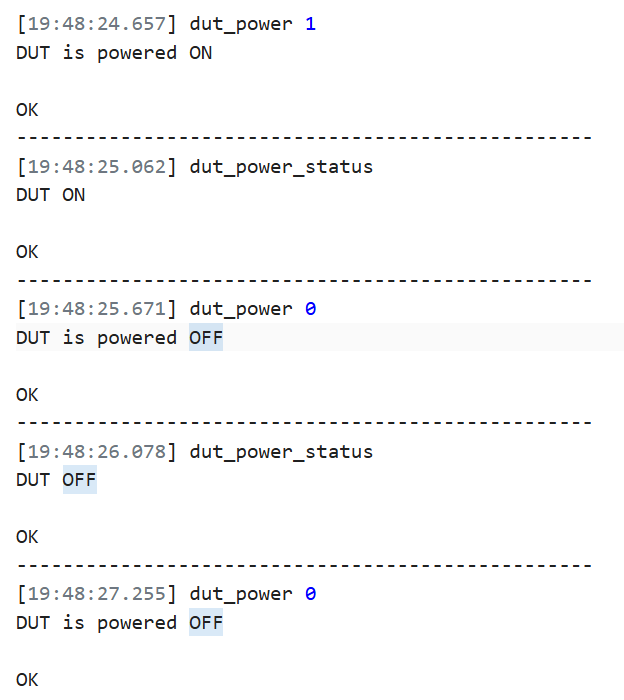
\includegraphics[width=0.85\textwidth]{image/hil_serial_log.png}
    \caption{File log giao tiếp serial giữa Robot Framework và HIL}
    \label{fig:hil_serial_log}
\end{figure}

Thông qua file log này, người phát triển có thể kiểm tra chính xác các lệnh đã được gửi xuống HIL cũng như dữ liệu phản hồi thực tế từ hệ thống phần cứng. Điều này đặc biệt hữu ích trong quá trình phân tích lỗi hoặc kiểm tra hoạt động của firmware DUT.



\newpage
\chapter{KẾT LUẬN VÀ HƯỚNG PHÁT TRIỂN}

\section{Kết luận}

Sau quá trình thực hiện đề tài, nhóm đã tích lũy được nhiều kiến thức và kỹ năng thực tiễn, góp phần hoàn thiện năng lực chuyên môn:
\begin{itemize}
    \item Về lý thuyết, củng cố lại kiến thức về các giao thức truyền thông của vi điều khiển. Tìm hiểu và ứng dụng thuật toán Fast Fourier Transform - FFT để phân tích các dạng sóng.
    \item Thiết kế phần cứng cần đưa ra các phương án và đánh giá ưu - nhược điểm của từng phương án từ đó lựa chọn giải pháp tối ưu nhất phù hợp với yêu cầu hệ thống.
    \item Về bố trí linh kiện trên mạch in, cần sắp xếp sao cho tối ưu nhằm đảm bảo tính ổn định và các thao tác đo đạc trong quá trình phát triển phần cứng.
    \item Về kỹ thuật lập trình, quá trình thực hiện đề tài giúp nhóm nắm vững kiến thức lập trình nền tảng, cách gỡ lỗi trong quá trình phát triển, đồng thời nâng cao hiểu biết về hệ điều hành thời gian thực RTOS.
    \item Học thêm một Framework mới (Robot Framework) hỗ trợ cho việc kiểm thử tự động cho các hệ thống.
\end{itemize}

Từ những kết quả đạt được, đề tài không chỉ mang lại giá trị học thuật mà còn giúp nhóm định hướng rõ hơn cho con đường phát triển nghề nghiệp trong lĩnh vực kỹ thuật và công nghệ cao.

\subsection{Ưu điểm của đề tài}
\begin{itemize}
    \item Hệ thống có khả năng mô phỏng được một số phần cứng như SPI Flash, I2C EEPROM, I2C RTC.
    \item Cung cấp đầy đủ các tín hiệu digital, analog và các chuẩn giao tiếp truyền thông.
    \item Có khả năng thu thập dữ liệu từ thiết bị DUT, hỗ trợ người dùng theo dõi và phân tích tín hiệu trong quá trình hoạt động.
    \item Tích hợp phần mềm điều khiển và bộ thư viện Robot Framework, hỗ trợ xây dựng kịch bản kiểm thử tự động và lưu trữ kết quả của từng lần kiểm thử khác nhau.
    \item Hỗ trợ điều khiển nguồn và nạp chương trình cho thiết bị DUT thông qua USB, không cần kết nối ST-Link.
\end{itemize}

\subsection{Khuyết điểm của đề tài}
\begin{itemize}
    \item Chưa thể mô phỏng được những tín hiệu có nhiễu vật lý như nút nhấn, encoder,\dots
    \item Đối với một số giao thức tốc độ cao như CAN hoặc SPI, tốc độ giao tiếp cần được giảm xuống để đảm bảo hệ thống có đủ thời gian xử lý và phản hồi dữ liệu chính xác bằng phần mềm.
    \item Baudrate của các giao thức như CAN, UART chưa thể hỗ trợ cấu hình linh động.
    \item Tần số lấy mẫu của Logic Analyzer vẫn còn giới hạn, ảnh hưởng đến khả năng thu thập và phân tích các tín hiệu có tốc độ cao.
\end{itemize}

Tóm lại, mặc dù hệ thống vẫn còn tồn tại một số hạn chế nhất định, nhưng nhìn chung các mục tiêu đề ra ban đầu của đề tài đã được đáp ứng đầy đủ.
Sự phối hợp giữa phần cứng và phần mềm được thực hiện ổn định, cho phép hệ thống hỗ trợ hiệu quả quá trình kiểm thử và mô phỏng thiết bị DUT.
Đồng thời, đề tài cũng tạo nền tảng để tiếp tục phát triển và mở rộng thêm các tính năng trong tương lai.

\section{Hướng phát triển}
Mặc dù đã đạt được các kết quả tích cực, hệ thống HIL trong đồ án vẫn còn nhiều tiềm năng để tiếp tục hoàn thiện và mở rộng trong tương lai. Một số hướng phát triển chính được đề xuất như sau:

\begin{itemize}
    \item Mở rộng khả năng mô phỏng nhiều phần cứng hơn như nhiệt độ, độ ẩm, gia tốc để tăng tính linh hoạt và ứng dụng thực tế.
    \item Tích hợp mạng cho hệ thống. Từ đó hệ thống sẽ hoạt động độc lập mà không cần phải kết nối trực tiếp với mày tính thông qua USB. Các dữ liệu thu thập sẽ được gửi về máy chủ để lưu trữ, giám sát và xử lý từ xa.
    \item Tích hợp hệ thống với các nền tảng quản lý phiên bản như Git nhằm hướng tới mô hình kiểm thử tự động hoàn toàn. Hệ thống có thể tự động phát hiện các pull request mới, tải mã nguồn về để biên dịch và thực hiện kiểm thử trên phần cứng thực tế.
    Sau khi toàn bộ bài kiểm thử đạt yêu cầu, hệ thống có thể tự động xác nhận và thực hiện merge, giúp tối ưu quy trình phát triển và kiểm thử phần mềm nhúng theo hướng CI/CD.
\end{itemize}



\newpage
\sloppy

\begin{thebibliography}{10}

\bibitem{hil_ni}
National Instruments, "What is Hardware-in-the-Loop (HIL)?",
\url{https://www.ni.com/en/solutions/transportation/hardware-in-the-loop/what-is-hardware-in-the-loop-.html}
(accessed: 12/5/2025).

\bibitem{can}
HQ Kvaser AB, "The CAN Bus Protocol Tutorial",
\url{https://kvaser.com/can-protocol-tutorial/}
(accessed: 12/5/2025).

\bibitem{rtos}
Jonathan Valvano, “Embedded Systems: Real-Time Operating Systems for ARM Cortex-M Microcontrollers”, 2017.

\bibitem{hil_ni}
Keysight Technologies, "What Is the Fourier Transform??", 
\url{https://www.keysight.com/used/us/en/knowledge/formulas/fourier-transform}
(accessed: 12/5/2025).

\bibitem{signal_process}
Sophocles J. Orfanidis, "Introduction to Signal and Processing", Rutgers University, 2010.

\bibitem{dsp}
Steven W. Smith, "The Scientist and Engineer's Guide to Digital Signal Processing", California Technical Publishing San Diego, 1999.

\bibitem{rm_f4}
STMicroelectronics, \textit{STM32F4x Series Reference Manual}, RM0090, 2023.

\bibitem{w25q}
Winbond Electronics Corporation, 
\textit{W25Q Series Serial Flash Memory Datasheet}, 2023.

\bibitem{ds1307}
Maxim Integrated, 
\textit{DS1307 I2C Real-Time Clock Datasheet}, 2016.

\bibitem{at24cxx}
Microchip Technology Inc., 
\textit{AT24Cxx I2C Serial EEPROM Datasheet}, 2018.

\end{thebibliography}


\end{document}
